%%%%%%%%%%%%%%%%%%%%%%%%%%%%%%%%%%%%%%%%%%%%%%%%%
%%%%%%%%% ARTICLE TEMPLATE LATEX %%%%%%%%%%%%%%%%
\documentclass[12pt,a4paper,final]{book}
%%%%%%%%%%%%%%%%%%%%%%%%%%%%%%%%%%%%%%%%%%%%%%%%%
%%%%%%%%%%%%%%%%%%%%%%%%%%%%%%%%%%%%%%%%%%%%%%%%%
\usepackage{fontspec}
\setmainfont[ Path = font/, 
UprightFont = *-Regular,
 BoldFont = *-Bold,
 ItalicFont = *-Italic]
{GentiumBookPlus}
% \setmainfont{Gentium Book Plus}
%%%%%%%%%%%%%%%%%%%%%%%%%%%%%%%%%%%%%%%%%%%%%%%%%
\usepackage{graphicx}
\graphicspath{{./Figures/}}
\usepackage{subfigure}

\usepackage{titling}

\usepackage[Conny]{fncychap}

\usepackage{latexsym}
\usepackage{xfrac}
% \usepackage{amssymb}
% include setspace package
\usepackage{setspace}

% include ams math package
\usepackage{amsmath}

% include fonts package
\usepackage{mathrsfs,amsfonts}

% include ams theorem package
\usepackage{amsthm,amsxtra}

% include the showkeys package
%\usepackage{showkeys}
\usepackage[final]{showkeys}

% include the stmaryrd package
% that contains many math symbols
\usepackage{stmaryrd}

\usepackage[makeroom]{cancel}
\usepackage{imakeidx}
\usepackage{tcolorbox}



% include the algorithm packages


\usepackage[sectionbib]{natbib}
\usepackage{chapterbib}
\renewcommand\bibname{Extended Reading}


\usepackage[ruled]{algorithm2e}
% \usepackage{algorithm}
% \usepackage{algorithmicx}
% \usepackage{algpseudocode}
\usepackage{mathtools}

% include pdftricks (pstricks version)

% \usepackage{pdftricks}
% \begin{psinputs}
% 	\usepackage{pstricks}
% 	\usepackage{pstcol}
% 	\usepackage{pst-plot}
% 	\usepackage{pst-tree}
% 	\usepackage{pst-eps}
% 	\usepackage{multido}
% 	\usepackage{pst-node}
% 	\usepackage{pst-eps}
% \end{psinputs}


% include hyperref package
% \ifPDF
\usepackage[debug,colorlinks=true, 
linkcolor=blue, bookmarksopen=false,
plainpages=false,pdfpagelabels]{hyperref}
% \else
% \usepackage[dvips]{hyperref}
% \fi

% use pdf version 1.6
% \pdfminorversion=6

\usepackage[openbib]{currvita}

% To define headers and footers
\usepackage{fancyhdr}

%%%%%%%%%%%%%%%%%%%%%%%%%%%
% define theorem type of commands
%%%%%%%%%%%%%%%%%%%%%%%%%%%

\newtheorem{theorem}{Theorem}[section]
\newtheorem{lemma}[theorem]{Lemma}
\newtheorem{definition}[theorem]{Definition}
\newtheorem{example}[theorem]{Example}
\newtheorem{exercise}[theorem]{Exercise}
\newtheorem{convention}[theorem]{Convention}
\newtheorem{statement}[theorem]{Statement}
\newtheorem{fact}[theorem]{Fact}
\newtheorem{axiom}[theorem]{Axiom}
\newtheorem{question}[theorem]{Question}
\newtheorem{proposition}[theorem]{Proposition} 
\newtheorem{remark}[theorem]{Remark} 
\newtheorem{corollary}[theorem]{Corollary} 
\newtheorem{problem}[theorem]{Problem} 
\newtheorem{notation}{Notation}
\newtheorem{assumption}{Assumption}

%%%%%%%%%%%%%%%%%%%%%%%%%%%%%%%%%%%%%%%%
% self-define operators
%%%%%%%%%%%%%%%%%%%%%%%%%%%%%%%%%%%%%%%%
\newcommand{\sgn}{\operatorname{sgn}}
\newcommand{\im}{\operatorname{im}}
\newcommand{\Char}{\operatorname{char}}
\newcommand{\supp}{\operatorname{supp}}
\newcommand{\singsupp}{\operatorname{singsupp}}
\newcommand{\diag}{{\rm diag}}
\newcommand{\dsum}{\displaystyle\sum}
\newcommand{\dint}{\displaystyle\int}
\newcommand{\eps}{\varepsilon}

% optimization 
\DeclareMathOperator*{\argmin}{\arg\min}
\DeclareMathOperator*{\argmax}{\arg\max}

% partial derivative
\newcommand{\pdr}[2]
{\dfrac{\partial{#1}}{\partial{#2}}}
\newcommand{\pdrr}[2]
{\dfrac{\partial^2{#1}}{\partial{#2}^2}}
\newcommand{\pdrt}[3]{\dfrac{\partial^2{#1}}
	{\partial{#2}{\partial{#3}}}}
\newcommand{\dr}[2]{\dfrac{d{#1}}{d{#2}}}
\newcommand{\drr}[2]{\dfrac{d^2{#1}}{d{#2}^2}}

% mathfrak symbols
\newcommand{\fT}{\mathfrak{T}}
\newcommand{\fu}{\mathfrak{u}}
\newcommand{\fo}{\mathfrak{o}}
\newcommand{\fU}{\mathfrak{U}}
\newcommand{\fO}{\mathfrak{O}}
\newcommand{\fE}{\mathfrak{E}}
\newcommand{\fm}{\mathfrak{m}}

% mathsf symbols
\newcommand{\sfc}{\mathsf c}
\newcommand{\sfC}{\mathsf C}

% mathbb symbols
\newcommand{\bbC}{\mathbb C} \newcommand{\bbE}{\mathbb E}
\newcommand{\bbL}{\mathbb L} \newcommand{\bbN}{\mathbb N}
\newcommand{\bbP}{\mathbb P} \newcommand{\bbQ}{\mathbb Q}
\newcommand{\bbR}{\mathbb R} \newcommand{\bbS}{\mathbb S}
\newcommand{\bbZ}{\mathbb Z} \newcommand{\scrE}{\mathscr{E}}

% mathbf symbols
\newcommand{\bzero}{{\mathbf 0}}
\newcommand{\btheta}{{\boldsymbol\theta}}
\newcommand{\btau}{\boldsymbol \tau}
\newcommand{\bchi}{\mbox{\boldmath{$\chi$}}}
\newcommand{\bnu}{{\boldsymbol \nu}}
\newcommand{\bmu}{\boldsymbol \mu}
\newcommand{\brho}{\mbox{\boldmath{$\rho$}}}
\newcommand{\bxi}{\boldsymbol \xi}
\newcommand{\bzeta}{\boldsymbol \zeta}
\newcommand{\bEta}{\boldsymbol \eta}
\newcommand{\bnabla}{\boldsymbol \nabla}
\newcommand{\blambda}{\boldsymbol \lambda}
\newcommand{\bLambda}{\boldsymbol \Lambda}
\newcommand{\bOmega}{\boldsymbol \Omega}
\newcommand{\bGamma}{\mbox{\boldmath{$\Gamma$}}}
\newcommand{\bSigma}{{\boldsymbol\Sigma}}
\newcommand{\bPi}{\boldsymbol \Pi}

\newcommand{\ba}{\mathbf a} \newcommand{\bb}{\mathbf b}
\newcommand{\bc}{\mathbf c} \newcommand{\bd}{\mathbf d}
\newcommand{\be}{\mathbf e} \newcommand{\bff}{\mathbf f}
\newcommand{\bg}{\mathbf g} \newcommand{\bh}{\mathbf h}
\newcommand{\bi}{\mathbf i} \newcommand{\bj}{\mathbf j}
\newcommand{\bk}{\mathbf k} \newcommand{\bl}{\mathbf l}
\newcommand{\bm}{\mathbf m} \newcommand{\bn}{\mathbf n}
\newcommand{\bo}{\mathbf o} \newcommand{\bp}{\mathbf p}
\newcommand{\bq}{\mathbf q} \newcommand{\br}{\mathbf r}
\newcommand{\bs}{\mathbf s} \newcommand{\bt}{\mathbf t}
\newcommand{\bu}{\mathbf u} \newcommand{\bv}{\mathbf v} 
\newcommand{\bw}{\mathbf w} \newcommand{\bx}{\mathbf x} 
\newcommand{\by}{\mathbf y} \newcommand{\bz}{\mathbf z} 
\newcommand{\bA}{\mathbf A} \newcommand{\bB}{\mathbf B}
\newcommand{\bC}{\mathbf C} \newcommand{\bD}{\mathbf D} 
\newcommand{\bE}{\mathbf E} \newcommand{\bF}{\mathbf F}
\newcommand{\bG}{\mathbf G} \newcommand{\bH}{\mathbf H}
\newcommand{\bI}{\mathbf I} \newcommand{\bJ}{\mathbf J}
\newcommand{\bK}{\mathbf K} \newcommand{\bL}{\mathbf L}
\newcommand{\bM}{\mathbf M} \newcommand{\bN}{\mathbf N}
\newcommand{\bO}{\mathbf O} \newcommand{\bP}{\mathbf P} 
\newcommand{\bQ}{\mathbf Q} \newcommand{\bR}{\mathbf R}
\newcommand{\bS}{\mathbf S} \newcommand{\bT}{\mathbf T}
\newcommand{\bU}{\mathbf U} \newcommand{\bV}{\mathbf V}
\newcommand{\bW}{\mathbf W} \newcommand{\bX}{\mathbf X} 
\newcommand{\bY}{\mathbf Y} \newcommand{\bZ}{\mathbf Z}

% mathcal symbols
\newcommand{\cA}{\mathcal A} \newcommand{\cB}{\mathcal B}
\newcommand{\cC}{\mathcal C} \newcommand{\cD}{\mathcal D} 
\newcommand{\cE}{\mathcal E} \newcommand{\cF}{\mathcal F}
\newcommand{\cG}{\mathcal G} \newcommand{\cH}{\mathcal H}
\newcommand{\cI}{\mathcal I} \newcommand{\cJ}{\mathcal J}
\newcommand{\cK}{\mathcal K} \newcommand{\cL}{\mathcal L}
\newcommand{\cM}{\mathcal M} \newcommand{\cN}{\mathcal N}
\newcommand{\cO}{\mathcal O} \newcommand{\cP}{\mathcal P} 
\newcommand{\cQ}{\mathcal Q} \newcommand{\cR}{\mathcal R}
\newcommand{\cS}{\mathcal S} \newcommand{\cT}{\mathcal T}
\newcommand{\cU}{\mathcal U} \newcommand{\cV}{\mathcal V}
\newcommand{\cW}{\mathcal W} \newcommand{\cX}{\mathcal X} 
\newcommand{\cY}{\mathcal Y} \newcommand{\cZ}{\mathcal Z}

%mathsf shortcuts -- for random variables
\newcommand{\sA}{\mathsf A} \newcommand{\sB}{\mathsf B}
\newcommand{\sC}{\mathsf C} \newcommand{\sD}{\mathsf D}
\newcommand{\sE}{\mathsf E} \newcommand{\sF}{\mathsf F}
\newcommand{\sG}{\mathsf G} \newcommand{\sH}{\mathsf H}
\newcommand{\sI}{\mathsf I} \newcommand{\sJ}{\mathsf J}
\newcommand{\sK}{\mathsf K} \newcommand{\sL}{\mathsf L}
\newcommand{\sM}{\mathsf M} \newcommand{\sN}{\mathsf N}
\newcommand{\sO}{\mathsf O} \newcommand{\sP}{\mathsf P}
\newcommand{\sQ}{\mathsf Q} \newcommand{\sR}{\mathsf R}
\newcommand{\sS}{\mathsf S} \newcommand{\sT}{\mathsf T}
\newcommand{\sU}{\mathsf U} \newcommand{\sV}{\mathsf V}
\newcommand{\sW}{\mathsf W} \newcommand{\sX}{\mathsf X}
\newcommand{\sY}{\mathsf Y} \newcommand{\sZ}{\mathsf Z}

% commonly-used probability notations
\newcommand{\prob}[1]{\bbP \negthinspace\left(#1\right)}
\newcommand{\rv}{random variable\ }
\newcommand{\expect}[1]{\bbE\!\left[#1\right]}
\DeclareMathOperator{\var}{Var}
\newcommand{\vari}[1]{\var\negthinspace\left[#1\right]}
\newcommand{\abs}[1]{|#1|}
\newcommand{\norm}[1]{\|#1\|}
%\newcommand{\E}[1]{\bbE\!\left[#1\right]}
\newcommand{\aver}[1]{\langle {#1} \rangle}
\newcommand{\Baver}[1]{\Big\langle {#1} \Big\rangle}
\newcommand{\fl}[1]{{\textsc{fl}}(#1)}
\newcommand{\tr}[1]{{\textrm{Tr}}(#1)}
%%%%%%%%%%%%%%%%%%%%%%%%%%%%%%%%%%%%%%%
\newcommand{\dd}[1]{{#1}''}% 2nd derivative
\newcommand{\mathtitle}[1]{\texorpdfstring{#1}{}}
%%%%%%%%%%%%%%%%%%%%%%%%%%%%%%%%%%%%%%%
%%%%%%%%%%%%%%%%%%%%%%
% setup page layout
%%%%%%%%%%%%%%%%%%%%%%
% pt - points (about 1/72 inch)
% pc - pica (12pt/pc 1/6 inch)
% in - inches (2.54cm/in)
% mm - millimeters 
% cm - centimeters 
% letter paper: 8.5 inch x 11.0 inch
\setlength\textwidth{39pc}
\setlength\textheight{52pc}
\setlength\hoffset{0pc}
\setlength\voffset{0pc}
\setlength\topmargin{0pt}
\setlength\headheight{0pt}
\setlength\headsep{50pt}
\setlength\oddsidemargin{0in}
\setlength\evensidemargin{0in}

%\addtolength\oddsidemargin{-1.2cm}
%\addtolength\evensidemargin{-1.2cm}
%\addtolength\topmargin{-1.5cm}

\setlength{\parindent}{0mm}
\setlength{\parskip}{1mm}

\newenvironment{keywords}
{\noindent{\bf Key words.}\small}{\par\vspace{1ex}}
\newenvironment{AMS}
{\noindent{\bf AMS subject classifications 2000.}\small}{\par}
\newenvironment{PACS}{\noindent{\bf PACS number(s):}\small}{\par}

\newcommand{\subtitle}[1]{%
  \posttitle{%
    \par\end{center}
    \begin{center}\large#1\end{center}
    \vskip0.5em}%
}


\makeatletter
\newcommand{\chapterauthor}[1]{%
	{\parindent0pt\vspace*{-25pt}%
		\linespread{1.1}\large\scshape#1%
		\par\nobreak\vspace*{35pt}}
	\@afterheading%
}
\makeatother
\title{Elementary Computational Mathematics}
\subtitle{Research Training Project}
\author{Yimin Zhong}
\date{\today}

\makeindex
\begin{document}
\maketitle
\frontmatter
\chapter*{Preface}

This note is the first component of the \emph{Research Training Project} (RTP).  The purpose is to provide a comprehensive introduction to basic computational mathematics for undergraduate and graduate students. 

\vspace{2cm}

{\centering { \Large\textsc{Prerequisites} }}

\begin{enumerate}
    \item Real Analysis, Complex Analysis, Functional Analysis, Harmonic Analysis (optional)
    \item Linear Algebra, Abstract Algebra, Representation Theory (optional) 
    \item Probability, Stochastic Processes
    \item Ordinary Differential Equations, Partial Differential Equations 
    \item Linear Programming, Convex Optimization
    \item Scientific Programming (MATLAB, Python, Julia, C/C++, Fortran, Rust, etc.)
    \item Lean (Proof Assistant Programming Language)
\end{enumerate}
\tableofcontents
\mainmatter
\part{Preliminaries}

\chapter{Floating Point Arithmetic}
\label{Ch: 1-Flo-Poi-Ari}

In this chapter, we will introduce some basics of the real number system for modern computers and discuss the arithmetic operations of the number system.

\section{Representation of Real Numbers}
\label{Sec: 1-Rep-Rea-Num}

Any \emph{nonzero} real number $x\in \bbR$ can be accurately represented with an infinite sequence of digits. This can be understood as the consequence that rational numbers are dense on any interval. Therefore, with the binary representation, we can write 
$$x = \pm (0.d_1 d_2 d_3\dots d_{t-1} d_t d_{t+1}\dots) \times 2^e,$$
where $e$ is an integer exponent and $d_1=1$, the other binary digits $d_i\in \{0, 1\}$. The mantissa part
$$0.d_1 d_2 d_3\dots =  \frac{d_1}{2} + \frac{d_2}{2^2} + \frac{d_3}{2^3} + \cdots.$$

\begin{remark}
    To guarantee the uniqueness of the above representation, we need a further assumption that there exists an infinite subset $S\subset \bbN$ that $d_j\neq 1$ for $j\in S$. For example, under binary representation
    $$0.111\dots = (0.1)\times 2^1,$$
    then we will take the latter representation.
\end{remark}

\section{Floating Point Numbers}
\label{Sec: 1-Flo-Poi-Num}

The floating point numbers generally refer to a set of real numbers with \emph{finite} mantissa length. More precisely, we consider the set of real numbers $\mathbb{F} = \mathbb{F}(t, e_{\min}, e_{\max})\subset \bbR$ that
$$\mathbb{F} := \{x\in \bbR\mid x = \pm (0.d_1 d_2 d_3\dots d_{t-1} d_t) \times 2^e, d_1 =1,  e_{\min}\le e\le e_{\max}\}\cup \{0\}.$$
It can be seen that there are only finite numbers in $\mathbb{F}$ with the smallest positive element $x_{\min} = 2^{e_{\min}-1}$ and the largest element $x_{\max} = ( 1- 2^{-t} )\times 2^{e_{\max} }$. Therefore $$\mathbb{F}\subset \overline{\mathbb{F}}:= \{ x\in \bbR\mid x_{\min} \le |x| \le x_{\max}\}\cup \{ 0\}.$$

\begin{remark}
    The elements in $\mathbb{F}$ are called normalized. If we allow $d_1 = 0$ in the definition of $\mathbb{F}$, then the numbers in the set are called denormalized.
\end{remark}

\begin{theorem}[Distribution of floating numbers]
\label{Thm: 1-Dis-flo-num}
    For any $e_{\min} \le e\le e_{\max}$, the distribution of the floating point number system $\mathbb{F}$ on interval $[2^{e-1}, 2^e]$ is equidistant with distances of length $2^{e-t}$.
\end{theorem}

\begin{proof}
    For any  $x \in \mathbb{F}\cap [2^{e-1}, 2^e]$ it can be represented by 
    $$x = (0.d_1d_2\dots d_t)\times 2^{e}$$
    where $d_1 = 1$. The mantissa is equidistantly distributed with distance $2^{-t}$, therefore the floating point numbers are equidistantly distributed with distances of length $2^{e-t}$. 
\end{proof}

To understand the approximation to real numbers by the floating point number system $\mathbb{F}$, it is important to consider the maximal relative distance between the numbers in $\overline{\mathbb{F}}$ and their respective closest element in $\mathbb{F}$, which is the following quantity:
$$\max_{x\in \overline{\mathbb{F}}, x\neq 0}\min_{z\in\mathbb{F}} \frac{|z - x|}{|x|}.$$
The following holds:
\begin{theorem}[Machine precision]
\label{Thm: 1-Mac-pre}
    $$\max_{x\in \overline{\mathbb{F}}, x\neq 0}\min_{z\in\mathbb{F}} \frac{|z - x|}{|x|}\le  2^{-t}.$$
    The number $\mathrm{u}:= 2^{-t}$ is also called rounding unit or machine precision.
\end{theorem}
\begin{proof}
    Without loss of generality, we only need to consider the positive numbers in $\overline{\mathbb{F}}$, then one can represent any nonzero $x\in [x_{\min}, x_{\max}]$ by
    $$x = (0.d_1 d_2 \dots d_t\dots)\times 2^e\in [2^{e-1}, 2^e].$$
    Since the floating point numbers are equidistantly distributed on $[2^{e-1}, 2^e]$ from Theorem~\ref{Thm: 1-Dis-flo-num}, one can find $z^{\ast}\in\mathbb{F}$ such that $$|z^{\ast} - x| \le \frac{1}{2} 2^{e-t},$$
    therefore 
    $$\frac{|z^{\ast}- x|}{|x|}\le \frac{1}{2} 2^{e-t} \frac{1}{2^{e-1}} = 2^{-t}.$$
\end{proof}

\begin{remark}
On modern computers, the following two floating point number systems $$\mathbb{F}_{32}:= \mathbb{F}(24, -125, 128),\quad\mathbb{F}_{64}:= \mathbb{F}(53, -1021, 1024)$$ are supported, they are often called single precision and double precision, respectively.  
\end{remark}

\section{Rounding}
\label{Sec: 1-Rou}
The rounding operation $\textsc{fl}$ is to map any real numbers of $\overline{\mathbb{F}}$ into the floating point number system $\mathbb{F}$ with the smallest error. Such rounding operation can be written out explicitly, let $ = \pm (0.d_1 d_2\dots d_t d_{t+1}\dots )\times 2^e$, then

\begin{equation*}
    \textsc{fl}(x) =\begin{cases}
        \pm (0.d_1 d_2\dots d_t) \times 2^e & \text{if } d_{t+1} = 0,\\
        \pm (0.d_1 d_2\dots d_t  + 2^{-t}) \times 2^e & \text{if } d_{t+1} = 1.
    \end{cases}
\end{equation*}
It is clear that rounding $\textsc{fl}$ is monotone and idempotent, which means
\begin{itemize}
    \item $x\le y \Rightarrow \textsc{fl}(x) \le \textsc{fl}(y)$. 
    \item $\textsc{fl}(z) = z$ if $z\in \mathbb{F}$.
\end{itemize}


\begin{theorem}[Rounding error]
\label{Thm: 1-Rou-err}
    For any $x\in \overline{\mathbb{F}}$, $|\textsc{fl}(x) - x| = \min_{z\in \mathbb{F}} |z - x|$. If $x\neq 0$, then
    $$\frac{|\textsc{fl}(x) - x|}{|x|}\le \mathrm{u} = 2^{-t}.$$
\end{theorem}

\begin{proof}
    The special case that $x = 0$ is trivial, we only consider $x\in [x_{\min}, x_{\max}]$, it can be seen that 
    \begin{equation*}
        |\textsc{fl}(x) - x| = | (0.d_1d_2\dots \tilde{d}_t) - (0.d_1d_2\dots d_t d_{t+1} \dots )|\times 2^e \le 2^{-(t+1)} \times 2^e,
    \end{equation*}
    where $\tilde{d}_t$ is the rounding bit, therefore 
    \begin{equation*}
        \frac{|\textsc{fl}(x) - x|}{|x|} \le \frac{2^{e-(t+1)}}{2^{e-1}} = 2^{-t}.
    \end{equation*}
\end{proof}

\begin{corollary}
\label{Cor: 1-Rel-err}
    For any $x\in\overline{\mathbb{F}}$, $\textsc{fl}(x) = x(1+\delta)$ with $|\delta|\le \mathrm{u}$.
\end{corollary}


\setlength\fboxsep{2pt}
\section{Arithmetic Operations}
\label{Sec: 1-Ari-Ope}
Let $\mathbb{F} = \mathbb{F}(t, e_{\min}, e_{\max})$ be a given floating point number system and we consider the basic binary operation $\circ\in \{ +, -, *, /\}$ on $\mathbb{F}$, to represent the outcome in $\mathbb{F}$, a straightforward realization is to define the binary operation $\boxed{\circ}$ as the following (for the case of division, we assume $y\neq 0$):
$$x \,\boxed{\circ}\, y := \textsc{fl}(x\circ y),$$
then for any $x, y\in\mathbb{F}$, if $x\circ y\in \overline{\mathbb{F}}$, then $x \,\boxed{\circ}\, y = (x\circ y)(1 + \delta)$ with $|\delta| \le \mathrm{u}$ from the Corollary~\ref{Cor: 1-Rel-err}.

\begin{remark}[Cancellation error]
\label{Rem: 1-Can-err}
    If $x, y\in\bbR$, then the relative error from the following binary operation $\textsc{fl}(x)\,\boxed{+}\,\textsc{fl}(y)$ can be estimated by
    \begin{equation*}
    \begin{aligned}
    \frac{|\textsc{fl}(x)\,\boxed{+}\,\textsc{fl}(y)- (x +  y) |}{|x + y|} &\le \frac{|\textsc{fl}(x)\,\boxed{+}\,\textsc{fl}(y) - (\textsc{fl}(x) +  \textsc{fl}(y)) |}{|x + y|} + \frac{| (\textsc{fl}(x) +  \textsc{fl}(y)) - (x+y)   |}{|x+y|}\\  
    &\le\mathrm{u} + (\mathrm{u} +\mathrm{u}^2) \frac{|x|+|y|}{|x+y|}.
    \end{aligned}
    \end{equation*}
    When $x$ and $y$ are close in magnitude but with opposite signs, the cancellation error will be significant.
\end{remark}
\subsection{Error Accumulation: Multiplication}
\label{SSec: 1-Err-Acc-Mul}
For complicated computations on modern computers, the errors from arithmetic operations will accumulate towards the final result (we do not consider techniques such as fused multiply-add (FMA) here). To quantify the accumulation effect, we will need the following lemma.

\begin{lemma}
\label{Lem: 1-Acc}
    For real numbers $a_1, a_2, \dots, a_n$ with $|a_k|\le \delta$ for $k=1,\dots, n$, then for $n\delta < 1$, the following holds
    $$\prod_{k=1}^n (1 + a_k) = 1 + b_n,$$
    where $|b_n| \le \frac{n\delta}{1 - n\delta}$.
\end{lemma}


\begin{proof}
    The proof is quite easy with induction. When $n=1$, $|b_1| = |a_1|\le \delta \le \frac{\delta}{1 - \delta}$. Suppose the claim holds for $n = m$, then for $n = m +1$, we could see that
    \begin{equation*}
        \prod_{k=1}^{m+1} (1 + a_k) = (1 + b_m) (1 + a_{m+1}) = 1 + b_{m+1}, 
    \end{equation*}
    which implies that $b_{m+1} = b_m + a_{m+1} + a_{m+1}b_m$, with the given bounds on $a_{m+1}$ and $b_m$, we can estimate
    \begin{equation*}
        |b_{m+1}| = | b_m + a_{m+1} + a_{m+1}b_m | \le \frac{(m+1)\delta}{1 - m\delta} \le \frac{(m+1)\delta}{1 - (m+1)\delta}.
    \end{equation*}
\end{proof}


Next, we consider the naive floating point product $P_n$ of $n$ real numbers $\{x_j\}_{j=1}^n \subset \bbR$ with assumption that $(2n-1)\textup{u} < 1$ by the following iteration
\begin{equation*}
    \begin{cases}
        P_k = \fl{x_1} & k=1,\\
        P_k = P_{k-1}~\boxed{\ast}~ \fl{x_k} & k\ge 2.
    \end{cases}
\end{equation*}
Let $\fl{x_k} = x_k(1 + \tau_k)$, then $|\tau_k|\le \textup{u}$. From the $n$-th iteration step $$P_n = P_{n-1}~\boxed{\ast}~ \fl{x_k} = \fl{\fl{P_{n-1}}\fl{x_n}} = \fl{P_{n-1}}\fl{x_n}(1 + \delta_n)$$ such that $|\delta_n|\le \textup{u}$, since $P_{n-1}\in \mathbb{F}$, $\fl{P_{n-1}} = P_{n-1}$, then 
\begin{equation*}
    \begin{aligned}
        P_n &= P_{n-1} \fl{x_n}(1 + \delta_n) = P_{n-2} \fl{x_{n-1}}(1 + \delta_{n-1}) (1 + \delta_k) = \cdots \\
        &=  \fl{x_1} \fl{x_2}\cdots \fl{x_n} \prod_{j=2}^n (1 + \delta_j) = \prod_{j=1}^n x_j (1 + \tau_j)  \prod_{j=2}^n (1 + \delta_j) \\
        &\le  (1 + \eta_n) \prod_{j=1}^n x_j,
    \end{aligned}
\end{equation*}
where $|\eta_n|\le \frac{(2n-1)\textup{u}}{1 - (2n-1)\textup{u}}$ by Lemma~\ref{Lem: 1-Acc}. 

\subsection{Error Accumulation: Addition}
\label{SSec: 1-Err-Acc-Add}
For naive floating point summation $S_n$ of $n$ real numbers $\{x_j \}_{j=1}^n$ by the iteration 
\begin{equation*}
    \begin{cases}
        S_k = 0 & k=0,\\
        S_k = S_{k-1}~\boxed{+}~ \fl{x_k} & k\ge 1,
    \end{cases}
\end{equation*}
we can carry out a similar analysis. Let $S^{\ast}_j = \sum_{k=1}^j x_k$ and  $\fl{x_k} = x_k ( 1 + \tau_k)$ for $|\tau_k|\le \textup{u}$, denote $\Delta S_j = S_j^{\ast} - S_j$, then
\begin{equation*}
    \begin{aligned}
        \Delta S_j &= S_j^{\ast} - S_j = S_{j}^{\ast} - ( S_{j-1}~\boxed{+}~ \fl{x_j}) \\
        &= \Delta S_{j-1}(1 + \delta_j) - \delta_j S_{j}^{\ast} - x_j\tau_j(1+\delta_j),
    \end{aligned}
\end{equation*}
where $|\tau_j|, |\delta_j|\le \textup{u}$. Therefore
\begin{equation*}
    \begin{aligned}
        |\Delta S_n|&\le |\Delta S_{n-1}|(1 + \textup{u}) + \textup{u} \sum_{k=1}^n |x_k| + |x_n| \textup{u}(1 + \textup{u}) \\
        &\le |\Delta S_{n-2}|(1 + \textup{u})^2 + \textup{u}(1+\textup{u})  \sum_{k=1}^j |x_k| + |x_j| \textup{u}(1 + \textup{u})^2 \\
        &\quad +  \textup{u} \sum_{k=1}^{j-1} |x_k| + |x_{j-1}| \textup{u}(1 + \textup{u})\\
        &\le  \cdots \\
        &\le  \sum_{l=1}^{n} \left( \textup{u}(1 + \textup{u})^{l-1} 
 \sum_{k=1}^l |x_k| + |x_{l}|\text{u}(1 + \textup{u})^{l-1} \right) \\
        & \le \sum_{l=1}^{n} \left( \textup{u}(1 + \textup{u})^{l-1} \sum_{k=1}^n |x_k|  \right) + \left(\sum_{l=1}^n |x_{l}|\right)\text{u}(1 + \textup{u})^{n-1}\\
        &= \left(\sum_{l=1}^n |x_{l}|\right) ((1 + \textup{u})^n - 1).
        \end{aligned}
\end{equation*}
Using the previous Lemma~\ref{Lem: 1-Acc} will provide an estimate of $ ((1 + \textup{u})^n - 1)$ as long as $n\textup{u} < 1$.

\section{Exercises}
\label{Sec: Exe-1}
Assume $n\in \bbN$ and $n\textup{u} < 1$, let $\{x_j\}_{j=1}^n$ be a sequence of real numbers, $\textsc{fl}:\overline{\mathbb{F}}\mapsto \mathbb{F}$ is the rounding operation, $\textup{u}$ is the machine epsilon. In the following, we briefly discuss the rounding error for floating point summation (sum reduction). 

\begin{definition}
    A reduction $\Pi$ of the floating point summation 
    $$\fl{x_1} ~\boxed{+}~ \fl{x_2} ~\boxed{+}~\cdots ~\boxed{+}~ \fl{x_n}$$ is an evaluation order for the $~\boxed{+}~$ operations. For example, $n = 4$, then the reduction $\Pi = (3,1,2)$ is corresponding to the following calculation
$$\fl{x_1} ~\boxed{+}~ \fl{x_2} + \underbrace{(\fl{x_3} ~\boxed{+}~ \fl{x_4})}_{=y_1}\to \underbrace{(\fl{x_1} ~\boxed{+}~ \fl{x_2})}_{=y_2} ~\boxed{+}~ y_1 \to \underbrace{(y_2 ~\boxed{+}~ y_1)}_{=y_3},$$
where $y_i$ denotes the result of $i$-th $\boxed{+}$ operation in the reduction. The final summation will be $y_{n-1}$. We denote $T_n(\Pi)$ as the result of floating point summation with reduction order $\Pi$.
\end{definition}


\subsection{Theoretical Part}
\begin{problem}
    Prove that the native summation has the following error estimate
    \begin{equation}
    |T_n(\Pi) - S_n|\le \left( \frac{\textup{u} n }{1 - \textup{u} n } \right)\sum_{j=1}^n |x_j|,
    \end{equation}
    where $S_n = \sum_{j=1}^n x_j$ and $\Pi = (1,2,\dots, (n-1))$.
\end{problem}

\begin{problem}
    Prove that
    \begin{equation}
    \min_{\Pi}|T_n(\Pi) - S_n| \le \left(\frac{ \textup{u} H }{1 - \textup{u} H  }\right)\sum_{j=1}^n |x_j|,
    \end{equation}
    where $H = \lceil\log_2 n \rceil$ and $T_n(\Pi)$ is the floating point summation with reduction order $\Pi$.
\end{problem}

\begin{problem}[Horner's scheme]
\label{Prb: 1-Theo-3}
The evaluation of polynomial 
    $$p(x) = a_0 + a_1 x + \dots + a_n x^n$$
is mostly using Horner's scheme, which writes the polynomial in `nested' form:
\begin{equation}
p(x) = a_0 + x (a_1 + x(a_2 + \dots x(a_{n-1} + x(a_n)))).
\end{equation}                                
Please find an upper bound of the rounding error for this scheme.         
\end{problem}

\subsection{Computational Part}

\begin{problem}[Pairwise summation]
    Based on the theoretical part, implement an algorithm for the summation $\sum_{j=1}^n x_j$ which has $\cO(\textup{u}\log_2 n)$ rounding error.
\end{problem}

\begin{problem}[Kahan compensated summation] 
\label{Prb: 1-Kahan-Sum}
Suppose $a, b\in\mathbb{R}$, the rounding error for the sum $s = \fl{\fl{a}+\fl{b}}$ ($a\ge b$) can be computed using 
    $$\fl{\fl{s - \fl{a}}-\fl{b}}$$
    Based on this property, one can keep track of the rounding error. 
\begin{algorithm}[!htb]
    \SetAlgoLined
    \caption{Kahan compensated summation}
    \KwData{$\{x_j\}_{j=1}^n\subset \mathbb{R}$}
    \KwResult{$s_n = \sum_{j=1}^n x_j$ }
    $j\gets 1$, $e_j \gets 0$, $s_j \gets x_j$ //    initialization; 
    \\
    \While{$j < n$}{
        $j\gets j + 1$\\
        $y_j = x_j - e_{j-1}$ //remove compensated error; \\ 
        $s_j = s_{j-1} + y_j$ //perform summation;\\
        $e_j = (s_j - s_{j-1}) - y_j$ //restore the rounding error;
    }
    \label{ALG: KAHAN}
\end{algorithm}
    Implement the Algorithm~\ref{ALG: KAHAN} described below and compare the accuracy with naive summation and pairwise summation with test cases.
\end{problem}


\begin{problem}
    Suppose the inputs $\{x_j\}_{j=1}^n\subset \mathbb{R}$ are randomly distributed (say $x_j\sim U(0,1)$ i.i.d), what is the estimated growth of the expected rounding error in terms of the total number of inputs $n$ for the naive summation and pairwise summation? Please explain your result. You can use Algorithm~\ref{ALG: KAHAN} as the accurate result approximately. 
\end{problem}
\newpage
% \section{Extended Reading}
\nocite{higham1993accuracy,higham2019new,muller2006elementary}
\bibliographystyle{apalike}
\bibliography{chap1}

\setcounter{chapter}{-1}
\chapter{Floating Point Arithmetic}
\label{Ch: 1-Flo-Poi-Ari}

In this chapter, we will introduce some basics of the real number system for modern computers and discuss the arithmetic operations of the number system.

\section{Representation of Real Numbers}
\label{Sec: 1-Rep-Rea-Num}

Any \emph{nonzero} real number $x\in \bbR$ can be accurately represented with an infinite sequence of digits. This can be understood as the consequence that rational numbers are dense on any interval. Therefore, with the binary representation, we can write 
$$x = \pm (0.d_1 d_2 d_3\dots d_{t-1} d_t d_{t+1}\dots) \times 2^e,$$
where $e$ is an integer exponent and $d_1=1$, the other binary digits $d_i\in \{0, 1\}$. The mantissa part
$$0.d_1 d_2 d_3\dots =  \frac{d_1}{2} + \frac{d_2}{2^2} + \frac{d_3}{2^3} + \cdots.$$

\begin{remark}
    To guarantee the uniqueness of the above representation, we need a further assumption that there exists an infinite subset $S\subset \bbN$ that $d_j\neq 1$ for $j\in S$. For example, under binary representation
    $$0.111\dots = (0.1)\times 2^1,$$
    then we will take the latter representation.
\end{remark}

\section{Floating Point Numbers}
\label{Sec: 1-Flo-Poi-Num}

The floating point numbers generally refer to a set of real numbers with \emph{finite} mantissa length. More precisely, we consider the set of real numbers $\mathbb{F} = \mathbb{F}(t, e_{\min}, e_{\max})\subset \bbR$ that
$$\mathbb{F} := \{x\in \bbR\mid x = \pm (0.d_1 d_2 d_3\dots d_{t-1} d_t) \times 2^e, d_1 =1,  e_{\min}\le e\le e_{\max}\}\cup \{0\}.$$
It can be seen that there are only finite numbers in $\mathbb{F}$ with the smallest positive element $x_{\min} = 2^{e_{\min}-1}$ and the largest element $x_{\max} = ( 1- 2^{-t} )\times 2^{e_{\max} }$. Therefore $$\mathbb{F}\subset \overline{\mathbb{F}}:= \{ x\in \bbR\mid x_{\min} \le |x| \le x_{\max}\}\cup \{ 0\}.$$

\begin{remark}
    The elements in $\mathbb{F}$ are called normalized. If we allow $d_1 = 0$ in the definition of $\mathbb{F}$, then the numbers in the set are called denormalized.
\end{remark}

\begin{theorem}[Distribution of floating numbers]
\label{Thm: 1-Dis-flo-num}
    For any $e_{\min} \le e\le e_{\max}$, the distribution of the floating point number system $\mathbb{F}$ on interval $[2^{e-1}, 2^e]$ is equidistant with distances of length $2^{e-t}$.
\end{theorem}

\begin{proof}
    For any  $x \in \mathbb{F}\cap [2^{e-1}, 2^e]$ it can be represented by 
    $$x = (0.d_1d_2\dots d_t)\times 2^{e}$$
    where $d_1 = 1$. The mantissa is equidistantly distributed with distance $2^{-t}$, therefore the floating point numbers are equidistantly distributed with distances of length $2^{e-t}$. 
\end{proof}

To understand the approximation to real numbers by the floating point number system $\mathbb{F}$, it is important to consider the maximal relative distance between the numbers in $\overline{\mathbb{F}}$ and their respective closest element in $\mathbb{F}$, which is the following quantity:
$$\max_{x\in \overline{\mathbb{F}}, x\neq 0}\min_{z\in\mathbb{F}} \frac{|z - x|}{|x|}.$$
The following holds:
\begin{theorem}[Machine precision]
\label{Thm: 1-Mac-pre}
    $$\max_{x\in \overline{\mathbb{F}}, x\neq 0}\min_{z\in\mathbb{F}} \frac{|z - x|}{|x|}\le  2^{-t}.$$
    The number $\mathrm{u}:= 2^{-t}$ is also called rounding unit or machine precision.
\end{theorem}
\begin{proof}
    Without loss of generality, we only need to consider the positive numbers in $\overline{\mathbb{F}}$, then one can represent any nonzero $x\in [x_{\min}, x_{\max}]$ by
    $$x = (0.d_1 d_2 \dots d_t\dots)\times 2^e\in [2^{e-1}, 2^e].$$
    Since the floating point numbers are equidistantly distributed on $[2^{e-1}, 2^e]$ from Theorem~\ref{Thm: 1-Dis-flo-num}, one can find $z^{\ast}\in\mathbb{F}$ such that $$|z^{\ast} - x| \le \frac{1}{2} 2^{e-t},$$
    therefore 
    $$\frac{|z^{\ast}- x|}{|x|}\le \frac{1}{2} 2^{e-t} \frac{1}{2^{e-1}} = 2^{-t}.$$
\end{proof}

\begin{remark}
On modern computers, the following two floating point number systems $$\mathbb{F}_{32}:= \mathbb{F}(24, -125, 128),\quad\mathbb{F}_{64}:= \mathbb{F}(53, -1021, 1024)$$ are supported, they are often called single precision and double precision, respectively.  
\end{remark}

\section{Rounding}
\label{Sec: 1-Rou}
The rounding operation $\textsc{fl}$ is to map any real numbers of $\overline{\mathbb{F}}$ into the floating point number system $\mathbb{F}$ with the smallest error. Such rounding operation can be written out explicitly, let $ = \pm (0.d_1 d_2\dots d_t d_{t+1}\dots )\times 2^e$, then

\begin{equation*}
    \textsc{fl}(x) =\begin{cases}
        \pm (0.d_1 d_2\dots d_t) \times 2^e & \text{if } d_{t+1} = 0,\\
        \pm (0.d_1 d_2\dots d_t  + 2^{-t}) \times 2^e & \text{if } d_{t+1} = 1.
    \end{cases}
\end{equation*}
It is clear that rounding $\textsc{fl}$ is monotone and idempotent, which means
\begin{itemize}
    \item $x\le y \Rightarrow \textsc{fl}(x) \le \textsc{fl}(y)$. 
    \item $\textsc{fl}(z) = z$ if $z\in \mathbb{F}$.
\end{itemize}


\begin{theorem}[Rounding error]
\label{Thm: 1-Rou-err}
    For any $x\in \overline{\mathbb{F}}$, $|\textsc{fl}(x) - x| = \min_{z\in \mathbb{F}} |z - x|$. If $x\neq 0$, then
    $$\frac{|\textsc{fl}(x) - x|}{|x|}\le \mathrm{u} = 2^{-t}.$$
\end{theorem}

\begin{proof}
    The special case that $x = 0$ is trivial, we only consider $x\in [x_{\min}, x_{\max}]$, it can be seen that 
    \begin{equation*}
        |\textsc{fl}(x) - x| = | (0.d_1d_2\dots \tilde{d}_t) - (0.d_1d_2\dots d_t d_{t+1} \dots )|\times 2^e \le 2^{-(t+1)} \times 2^e,
    \end{equation*}
    where $\tilde{d}_t$ is the rounding bit, therefore 
    \begin{equation*}
        \frac{|\textsc{fl}(x) - x|}{|x|} \le \frac{2^{e-(t+1)}}{2^{e-1}} = 2^{-t}.
    \end{equation*}
\end{proof}

\begin{corollary}
\label{Cor: 1-Rel-err}
    For any $x\in\overline{\mathbb{F}}$, $\textsc{fl}(x) = x(1+\delta)$ with $|\delta|\le \mathrm{u}$.
\end{corollary}


\setlength\fboxsep{2pt}
\section{Arithmetic Operations}
\label{Sec: 1-Ari-Ope}
Let $\mathbb{F} = \mathbb{F}(t, e_{\min}, e_{\max})$ be a given floating point number system and we consider the basic binary operation $\circ\in \{ +, -, *, /\}$ on $\mathbb{F}$, to represent the outcome in $\mathbb{F}$, a straightforward realization is to define the binary operation $\boxed{\circ}$ as the following (for the case of division, we assume $y\neq 0$):
$$x \,\boxed{\circ}\, y := \textsc{fl}(x\circ y),$$
then for any $x, y\in\mathbb{F}$, if $x\circ y\in \overline{\mathbb{F}}$, then $x \,\boxed{\circ}\, y = (x\circ y)(1 + \delta)$ with $|\delta| \le \mathrm{u}$ from the Corollary~\ref{Cor: 1-Rel-err}.

\begin{remark}[Cancellation error]
\label{Rem: 1-Can-err}
    If $x, y\in\bbR$, then the relative error from the following binary operation $\textsc{fl}(x)\,\boxed{+}\,\textsc{fl}(y)$ can be estimated by
    \begin{equation*}
    \begin{aligned}
    \frac{|\textsc{fl}(x)\,\boxed{+}\,\textsc{fl}(y)- (x +  y) |}{|x + y|} &\le \frac{|\textsc{fl}(x)\,\boxed{+}\,\textsc{fl}(y) - (\textsc{fl}(x) +  \textsc{fl}(y)) |}{|x + y|} \\&\quad + \frac{| (\textsc{fl}(x) +  \textsc{fl}(y)) - (x+y)   |}{|x+y|}\\  
    &\le\mathrm{u} + (\mathrm{u} +\mathrm{u}^2) \frac{|x|+|y|}{|x+y|}.
    \end{aligned}
    \end{equation*}
    When $x$ and $y$ are close in magnitude but with opposite signs, the cancellation error will be significant.
\end{remark}
\subsection{Error Accumulation: Multiplication}
\label{SSec: 1-Err-Acc-Mul}
For complicated computations on modern computers, the errors from arithmetic operations will accumulate towards the final result (we do not consider techniques such as fused multiply-add (FMA) here). To quantify the accumulation effect, we will need the following lemma.

\begin{lemma}
\label{Lem: 1-Acc}
    For real numbers $a_1, a_2, \dots, a_n$ with $|a_k|\le \delta$ for $k=1,\dots, n$, then for $n\delta < 1$, the following holds
    $$\prod_{k=1}^n (1 + a_k) = 1 + b_n,$$
    where $|b_n| \le \frac{n\delta}{1 - n\delta}$.
\end{lemma}


\begin{proof}
    The proof is quite easy with induction. When $n=1$, $|b_1| = |a_1|\le \delta \le \frac{\delta}{1 - \delta}$. Suppose the claim holds for $n = m$, then for $n = m +1$, we could see that
    \begin{equation*}
        \prod_{k=1}^{m+1} (1 + a_k) = (1 + b_m) (1 + a_{m+1}) = 1 + b_{m+1}, 
    \end{equation*}
    which implies that $b_{m+1} = b_m + a_{m+1} + a_{m+1}b_m$, with the given bounds on $a_{m+1}$ and $b_m$, we can estimate
    \begin{equation*}
        |b_{m+1}| = | b_m + a_{m+1} + a_{m+1}b_m | \le \frac{(m+1)\delta}{1 - m\delta} \le \frac{(m+1)\delta}{1 - (m+1)\delta}.
    \end{equation*}
\end{proof}


Next, we consider the naive floating point product $P_n$ of $n$ real numbers $\{x_j\}_{j=1}^n \subset \bbR$ with assumption that $(2n-1)\textup{u} < 1$ by the following iteration
\begin{equation*}
    \begin{cases}
        P_k = \fl{x_1} & k=1,\\
        P_k = P_{k-1}~\boxed{\ast}~ \fl{x_k} & k\ge 2.
    \end{cases}
\end{equation*}
Let $\fl{x_k} = x_k(1 + \tau_k)$, then $|\tau_k|\le \textup{u}$. From the $n$-th iteration step $$P_n = P_{n-1}~\boxed{\ast}~ \fl{x_k} = \fl{\fl{P_{n-1}}\fl{x_n}} = \fl{P_{n-1}}\fl{x_n}(1 + \delta_n)$$ such that $|\delta_n|\le \textup{u}$, since $P_{n-1}\in \mathbb{F}$, $\fl{P_{n-1}} = P_{n-1}$, then 
\begin{equation*}
    \begin{aligned}
        P_n &= P_{n-1} \fl{x_n}(1 + \delta_n) = P_{n-2} \fl{x_{n-1}}(1 + \delta_{n-1}) (1 + \delta_k) = \cdots \\
        &=  \fl{x_1} \fl{x_2}\cdots \fl{x_n} \prod_{j=2}^n (1 + \delta_j) = \prod_{j=1}^n x_j (1 + \tau_j)  \prod_{j=2}^n (1 + \delta_j) \\
        &\le  (1 + \eta_n) \prod_{j=1}^n x_j,
    \end{aligned}
\end{equation*}
where $|\eta_n|\le \frac{(2n-1)\textup{u}}{1 - (2n-1)\textup{u}}$ by Lemma~\ref{Lem: 1-Acc}. 

\subsection{Error Accumulation: Addition}
\label{SSec: 1-Err-Acc-Add}
For naive floating point summation $S_n$ of $n$ real numbers $\{x_j \}_{j=1}^n$ by the iteration 
\begin{equation*}
    \begin{cases}
        S_k = 0 & k=0,\\
        S_k = S_{k-1}~\boxed{+}~ \fl{x_k} & k\ge 1,
    \end{cases}
\end{equation*}
we can carry out a similar analysis. Let $S^{\ast}_j = \sum_{k=1}^j x_k$ and  $\fl{x_k} = x_k ( 1 + \tau_k)$ for $|\tau_k|\le \textup{u}$, denote $\Delta S_j = S_j^{\ast} - S_j$, then
\begin{equation*}
    \begin{aligned}
        \Delta S_j &= S_j^{\ast} - S_j = S_{j}^{\ast} - ( S_{j-1}~\boxed{+}~ \fl{x_j}) \\
        &= \Delta S_{j-1}(1 + \delta_j) - \delta_j S_{j}^{\ast} - x_j\tau_j(1+\delta_j),
    \end{aligned}
\end{equation*}
where $|\tau_j|, |\delta_j|\le \textup{u}$. Therefore
\begin{equation*}
    \begin{aligned}
        |\Delta S_n|&\le |\Delta S_{n-1}|(1 + \textup{u}) + \textup{u} \sum_{k=1}^n |x_k| + |x_n| \textup{u}(1 + \textup{u}) \\
        &\le |\Delta S_{n-2}|(1 + \textup{u})^2 + \textup{u}(1+\textup{u})  \sum_{k=1}^j |x_k| + |x_j| \textup{u}(1 + \textup{u})^2 \\
        &\quad +  \textup{u} \sum_{k=1}^{j-1} |x_k| + |x_{j-1}| \textup{u}(1 + \textup{u})\\
        &\le  \cdots \\
        &\le  \sum_{l=1}^{n} \left( \textup{u}(1 + \textup{u})^{l-1} 
 \sum_{k=1}^l |x_k| + |x_{l}|\text{u}(1 + \textup{u})^{l-1} \right) \\
        & \le \sum_{l=1}^{n} \left( \textup{u}(1 + \textup{u})^{l-1} \sum_{k=1}^n |x_k|  \right) + \left(\sum_{l=1}^n |x_{l}|\right)\text{u}(1 + \textup{u})^{n-1}\\
        &= \left(\sum_{l=1}^n |x_{l}|\right) ((1 + \textup{u})^n - 1).
        \end{aligned}
\end{equation*}
Using the previous Lemma~\ref{Lem: 1-Acc} will provide an estimate of $ ((1 + \textup{u})^n - 1)$ as long as $n\textup{u} < 1$.

\section{Exercises}
\label{Sec: Exe-1}
Assume $n\in \bbN$ and $n\textup{u} < 1$, let $\{x_j\}_{j=1}^n$ be a sequence of real numbers, $\textsc{fl}:\overline{\mathbb{F}}\mapsto \mathbb{F}$ is the rounding operation, $\textup{u}$ is the machine epsilon. In the following, we briefly discuss the rounding error for floating point summation (sum reduction). 

\begin{definition}
    A reduction $\Pi$ of the floating point summation 
    $$\fl{x_1} ~\boxed{+}~ \fl{x_2} ~\boxed{+}~\cdots ~\boxed{+}~ \fl{x_n}$$ is an evaluation order for the $~\boxed{+}~$ operations. For example, $n = 4$, then the reduction $\Pi = (3,1,2)$ is corresponding to the following calculation
$$\fl{x_1} ~\boxed{+}~ \fl{x_2} + \underbrace{(\fl{x_3} ~\boxed{+}~ \fl{x_4})}_{=y_1}\to \underbrace{(\fl{x_1} ~\boxed{+}~ \fl{x_2})}_{=y_2} ~\boxed{+}~ y_1 \to \underbrace{(y_2 ~\boxed{+}~ y_1)}_{=y_3},$$
where $y_i$ denotes the result of $i$-th $\boxed{+}$ operation in the reduction. The final summation will be $y_{n-1}$. We denote $T_n(\Pi)$ as the result of floating point summation with reduction order $\Pi$.
\end{definition}


\subsection{Theoretical Part}
\begin{problem}
    Prove that the native summation has the following error estimate
    \begin{equation}
    |T_n(\Pi) - S_n|\le \left( \frac{\textup{u} n }{1 - \textup{u} n } \right)\sum_{j=1}^n |x_j|,
    \end{equation}
    where $S_n = \sum_{j=1}^n x_j$ and $\Pi = (1,2,\dots, (n-1))$.
\end{problem}

\begin{problem}
    Prove that
    \begin{equation}
    \min_{\Pi}|T_n(\Pi) - S_n| \le \left(\frac{ \textup{u} H }{1 - \textup{u} H  }\right)\sum_{j=1}^n |x_j|,
    \end{equation}
    where $H = \lceil\log_2 n \rceil$ and $T_n(\Pi)$ is the floating point summation with reduction order $\Pi$.
\end{problem}

\begin{problem}[Horner's scheme]
\label{Prb: 1-Theo-3}
The evaluation of polynomial 
    $$p(x) = a_0 + a_1 x + \dots + a_n x^n$$
is mostly using Horner's scheme, which writes the polynomial in `nested' form:
\begin{equation}
p(x) = a_0 + x (a_1 + x(a_2 + \dots x(a_{n-1} + x(a_n)))).
\end{equation}                                
Please find an upper bound of the rounding error for this scheme.         
\end{problem}

\subsection{Computational Part}
The sample codes and test cases are available on GitHub. 
\begin{problem}[Pairwise summation]
    Based on the theoretical part, implement an algorithm for the summation $\sum_{j=1}^n x_j$ which has $\cO(\textup{u}\log_2 n)$ rounding error.
\end{problem}

\begin{problem}[Kahan compensated summation] 
\label{Prb: 1-Kahan-Sum}
Suppose $a, b\in\mathbb{R}$, the rounding error for the sum $s = \fl{\fl{a}+\fl{b}}$ ($a\ge b$) can be computed using 
    $$\fl{\fl{s - \fl{a}}-\fl{b}}$$
    Based on this property, one can keep track of the rounding error. 
\begin{algorithm}[!htb]
    \SetAlgoLined
    \caption{Kahan compensated summation}
    \KwData{$\{x_j\}_{j=1}^n\subset \mathbb{R}$}
    \KwResult{$s_n = \sum_{j=1}^n x_j$ }
    $j\gets 1$, $e_j \gets 0$, $s_j \gets x_j$ //    initialization; 
    \\
    \While{$j < n$}{
        $j\gets j + 1$\\
        $y_j = x_j - e_{j-1}$ //remove compensated error; \\ 
        $s_j = s_{j-1} + y_j$ //perform summation;\\
        $e_j = (s_j - s_{j-1}) - y_j$ //restore the rounding error;
    }
    \label{ALG: KAHAN}
\end{algorithm}
    Implement the Algorithm~\ref{ALG: KAHAN} described below and compare the accuracy with naive summation and pairwise summation with test cases.
\end{problem}


\begin{problem}
    Suppose the inputs $\{x_j\}_{j=1}^n\subset \mathbb{R}$ are randomly distributed (say $x_j\sim U(0,1)$ i.i.d), what is the estimated growth of the expected rounding error in terms of the total number of inputs $n$ for the naive summation and pairwise summation? Please explain your result. You can use Algorithm~\ref{ALG: KAHAN} as the accurate result approximately. 
\end{problem}
\newpage
% \section{Extended Reading}
\nocite{higham1993accuracy,higham2019new,muller2006elementary}
\bibliographystyle{apalike}
\bibliography{chap0}

\chapter{Interpolation}
\label{Ch: 2-Int}

The interpolation solves problems of the following type:

\begin{quotation}
    Given a set of predefined functions $\cK$, find an element $f: \mathbb{I}\mapsto \bbR$ in $\cK$ such that
    $y_j = f(x_j)$ for all $j=0,\dots, n$.
\end{quotation}
Here, $\mathbb{I}$ denotes a finite or infinite interval such that $x_1,\dots x_n\in \mathbb{I}$. One of the important applications for interpolation is computer-assisted design (CAD), which is used extensively in the manufacturing industry. Generally speaking, the interpolation provides a closed form of the function to determine the value of $y$ where the parameter $x$ is not accessible.

\section{Polynomial Interpolation}
\label{Sec: 2-Pol-Int}
The polynomial interpolation considers the set $\cK = \Pi_m$, where the set $\Pi_m$ represents the polynomials of degree $ \le m$. We will seek for a polynomial $f(x)$ with the constraints that
\begin{equation}\nonumber
    \begin{cases}
        f\in \cK = \Pi_n,&\\
        f(x_k) = y_k &\text{ for } k = 0, 1,\dots, n.
    \end{cases}
\end{equation}
The points $x_k$ are called \emph{interpolation nodes}, if $m > n$ (resp. $m < n$), the problem is underdetermined (resp. overdetermined). For the case that $ m = n$, we have
\begin{theorem}
\label{Thm: 2-Uni-Exi}
    There exists a unique polynomial function $f\in \Pi_n$ such that $f(x_j) = y_j$ for $j=0,\dots, n$.
\end{theorem}
\begin{proof}
   \noindent \emph{Existence: }In order to construct the polynomial $f$, it is straightforward to consider the general form of polynomial $f(x) = \sum_{j=0}^n a_j x^j$, then we can formulate a linear system for the coefficients $a_j$, $j=0,\dots, n$, which is 
    \begin{equation*}
        \begin{pmatrix}
            1 & x_0 & x_0^2 & \dots & x_0^n \\
            1 & x_1 & x_1^2 & \dots & x_1^n \\
            \vdots & \vdots &\vdots & \ddots & \vdots\\
            1 & x_n & x_n^2 & \dots & x_n^n
        \end{pmatrix} \begin{pmatrix}
            a_0\\a_1\\\vdots\\a_n
        \end{pmatrix} = \begin{pmatrix}
            y_0\\y_1\\\vdots \\y_n
        \end{pmatrix}.
    \end{equation*}
    The matrix 
    $$V = \begin{pmatrix}
        1 & x_0 & x_0^2 & \dots & x_0^n \\
        1 & x_1 & x_1^2 & \dots & x_1^n \\
        \vdots & \vdots &\vdots & \ddots & \vdots\\
        1 & x_n & x_n^2 & \dots & x_n^n
    \end{pmatrix} $$
    is called \emph{Vandermonde matrix}.
    To determine the coefficients $a_j$, the matrix $V$ must be invertible. Its determinant can be computed (try to prove it) as
    \begin{eqnarray}
        \det(V) = \prod_{0\le i\le j\le n}(x_j - x_i).
    \end{eqnarray}
    When $\{x_j\}_{j=0}^n$ are distinct, the determinant is nonzero.

   \noindent \emph{Uniqueness: }
    Suppose there are two distinct polynomials $f, g\in \Pi_n$ satisfying the condition that $f(x_j) = g(x_j) = y_j$, then $f - g$ has $(n+1)$ roots $x_j$, $j=0, \dots, n$. If $f\neq g$, it is clear that $f-g\in\Pi_n$ has at most $n$ roots. Contradiction.
\end{proof}

In the above proof, the interpolation polynomial can be uniquely determined by solving the linear system 
$$\begin{pmatrix}
    1 & x_0 & x_0^2 & \dots & x_0^n \\
    1 & x_1 & x_1^2 & \dots & x_1^n \\
    \vdots & \vdots &\vdots & \ddots & \vdots\\
    1 & x_n & x_n^2 & \dots & x_n^n
\end{pmatrix} \begin{pmatrix}
    a_0\\a_1\\\vdots\\a_n
\end{pmatrix} = \begin{pmatrix}
    y_0\\y_1\\\vdots \\y_n
\end{pmatrix}.$$ 
However, it is generally easier to compute the polynomial $f$ with the \emph{Lagrange polynomial interpolation} (which is somewhat equivalent to computing the inverse of $V$).
\subsection{Lagrange Polynomial}
\begin{definition}
    For the given distinct $x_j$, $j = 0, 1, \dots, n$, the Lagrange polynomials $L_j\in\Pi_n$, $j=0,1,\dots, n$ are defined by 
    \begin{equation}
        L_j(x) = \prod_{s = 0, s\neq j}^n \frac{x - x_s}{x_j - x_s}, \quad j = 0, 1,\dots , n.
    \end{equation}
\end{definition}
It is clear that these polynomials satisfy the conditions that 
\begin{equation}
    L_j(x_k) = \delta_{jk} := \begin{cases}
        1&\text{for } k=j,\\
        0&\text{for } k\neq j.
    \end{cases}
\end{equation}
Therefore these polynomials are linearly independent, which form a basis of the $(n+ 1)$-dimensional space $\Pi_n$.
\begin{theorem}
\label{Thm: 2-Uni-Exi-Lag}
    The unique interpolating polynomial $f$ satisfying $f(x_j) = y_j$, $j=0,1,\dots, n$ can be represented by 
    \begin{equation}
        f(x) = \sum_{j=0}^n y_j L_j(x).
    \end{equation}
\end{theorem}
\begin{proof}
    It is straightforward to check the interpolation conditions are satisfied.
\end{proof}
\begin{remark}
    We introduce a preliminary procedure to compute the value of the interpolating polynomial $f$ at a point $x$. Let the constants $k_j$ and $q(x)$ be defined as 
    \begin{equation}
        k_j = \prod_{s= 0, s\neq j}\frac{1}{x_j - x_s},\quad q(x) = \prod_{j=0}^n (x - x_j),
    \end{equation}
    then 
    \begin{equation}
        f(x) = \sum_{j=0}^n y_j L_j(x) = q(x)  \sum_{j=0}^n k_j y_j \frac{1}{x - x_j}.
    \end{equation}
    One can first compute $k_j$ with $\cO(n^2)$ flops, then $f(x)$ can be computed with $\cO(n)$ flops. The advantage of the above scheme is the constants $k_j$ are independent of $y_j$, therefore evaluating another instance of the interpolating polynomial will not need to re-compute them. The disadvantage is that if we add a new node, the constants $k_j$ must be updated with an additional cost of $\cO(n)$ flops. Later we will see if Newton's form can overcome this issue.
\end{remark}
\subsection{Interpolation Error}
\label{SSec: 2-Int-Err}
When the data pairs $(x_j, y_j)$, $j=0,1,\dots, n$ are generated by a sufficiently smooth function $h(x)$, it is possible to quantify the error between the interpolating polynomial $f(x)$ and $h(x)$. 
\begin{theorem}
\label{Thm: 2-Int-err}
    Let $h: [a, b]\mapsto \bbR$ be a $(n+1)$-times differentiable function. If $f(x)\in\Pi_n$ is the interpolating polynomial that 
    $$f(x_j) = h(x_j),$$
    for $j=0,1,\dots, n$. Then, for each $\overline{x}\in [a, b]$, the error can be represented by 
    \begin{equation}
        h(\overline{x}) - f(\overline{x}) = \frac{\omega(\overline{x})}{(n+1)!} h^{(n+1)}(\xi),
    \end{equation}
    where $\xi = \xi(\overline{x})\in [a, b]$ and $\omega(x) = \prod_{j=0}^n (x - x_j)$.
\end{theorem}
\begin{proof}
    The proof is based on Rolle's Theorem. Select any $\overline{x}\in[a, b]$ such that $\omega(\overline{x})\neq 0$, then let 
    $$\psi(x) = h(x) - f(x) - k\omega (x),$$
    the constant $k$ is chosen such that $\psi(\overline{x}) = 0$. Then $\psi(x) = 0$ at $(n+2)$ points, 
    $$x_0, x_1, \dots, x_n, \overline{x}\in [a, b].$$
    By Rolle's Theorem, $\psi^{(n+1)}$ has at least one zero $\xi$ in $[a,b]$. Therefore,
    \begin{equation}
        \psi^{(n+1)}(\xi) = h^{(n+1)}(\xi) - 0 - k(n+1)! = 0.
    \end{equation}
\end{proof}

\begin{corollary}
    If $h(x)\in C^{\infty}([a, b])$ satisfies that $\max_{x\in[a,b]} |h^{(n)}(x)|\le M <\infty$ for all $n\ge 0$, then the interpolating polynomial approximates $h$ uniformly as the number of nodes $n\to \infty$.
\end{corollary}
\begin{proof}
    Since $|x -x_j|\le b-a$, the error is bounded by $\frac{(b-a)^{n+1}}{(n+1)!} M$, which converges to zero.
\end{proof}
It is interesting to think about the converse: under what condition does the interpolation error not vanish as the number of nodes tends to infinity? From Theorem~\ref{Thm: 2-Int-err}, the error depends on the sizes of three terms. 
\begin{enumerate}
    \item The bound of the $(n+1)$-th derivative, $\max_{x\in[a,b]}|h^{(n+1)}(x)|$. This could proliferate. For example, $h(x) = x^{-\sfrac{1}{2}}$ on $[\sfrac{1}{2}, \sfrac{3}{2}]$,
    \begin{equation}
         h^{(n+1)}(x) = \frac{(-1)^{n+1}}{2^{n+1}} (2n+1)!! x^{-(2n+3)/2}.
    \end{equation}
    \item The function $\omega(x) = \prod_{j=0}^n (x - x_j)$, such a product, could be large if $x$ and the nodes $x_j$ are not so close.
    \item The term $\frac{1}{(n+1)!}$, which decays fast.
\end{enumerate}
We can see that for the function $h(x) = x^{-\sfrac{1}{2}}$ on $[\sfrac{1}{2}, \sfrac{3}{2}]$, it is not trivial to show the interpolating polynomial could converge to $h$ anymore (although it is still true for certain choices of $x_j$, see Exercise~\ref{Prb: 2-Theo-2}). 

Next, we try to provide a better estimate of $\omega$ for the special choice: equally spaced nodes.  Let the nodes $x_j = a + j\Delta$, where $\Delta = \frac{b-a}{n}$. It is not difficult (prove it) to see $\omega(x)$ will be the worst if $x$ is located on the end sub-intervals, $[x_0, x_1]$ and $[x_{n-1}, x_n]$. Without loss of generality, we assume $x$ is located on $[x_0, x_1]$, then 
$$|x - x_j|\le j \Delta$$
for $j = 2, \dots, n$, which implies 
\begin{equation}
\label{EQ: MAX-OMEGA}
    |\omega(x)|\le \prod_{j=0}^n |x - x_j|\le n! \Delta^{n-1} \sup_{x\in [x_0, x_1]} |(x - x_0)(x-x_1)|= \frac{n!}{4} \frac{(b-a)^{n+1}}{n^{n+1}},
\end{equation}
Thus interpolation error is bounded by
$$  \|h  - f\|_{\infty} \le  \frac{\sup_{x\in[a,b]}|h^{(n+1)}(x)|}{4(n+1)} \frac{(b-a)^{n+1}}{n^{n+1}}.$$
Such an estimate is useful to derive uniform convergence. 
\begin{example}
    Consider $h(x) = x^{-1}$ on $[\sfrac{1}{2}, \sfrac{3}{2}]$. Then $h^{(n+1)}(x) = \frac{(n+1)!(-1)^{n+1}}{x^{n+2}}$, hence 
    \begin{equation}
        \frac{| h^{(n+1)}(x) |}{4(n+1)}  \frac{(b-a)^{n+1}}{n^{n+1}} \le \frac{1}{4n^{n+1}}\max_{x\in[\sfrac{1}{2}, \sfrac{3}{2}]} \left| \frac{1}{x^{n+2}} \right| = \frac{1}{2} \left(\frac{2}{n}\right)^{n+1},
    \end{equation}
    therefore, the interpolation error converges to zero exponentially. It is important to notice that the above method only works for intervals away from the origin. 
\end{example} 

\subsection{Runge's Phenomenon}
\label{SSec: 2-Run-Phe}
From the above discussion, we can see there is a possibility that $\max_{x\in[a,b]}|h^{n+1}(x)|$ grows much faster than $n^{n+2}$, which would lead to divergence. Hence, increasing the number of interpolation nodes (at least for equally spaced nodes) is not guaranteed for better approximation. The most famous example is the one made by Carl Runge. 
\begin{equation}
\label{EQ: RUNGE-EXAMPLE}
    h(x) = \frac{1}{1+x^2},\quad x\in [-5, 5].
\end{equation} 
\begin{figure}[!htb]
    \centering
    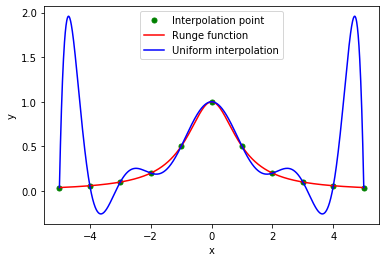
\includegraphics[scale=0.7]{runge.png}
    \caption{Runge's phenomenon. Interpolation with 11 equally spaced nodes. }
\end{figure}
It can be shown that the interpolation will diverge at around $3.63$ as $n\to \infty$ and the maximum error $\max_{x\in[-5, 5]} |f_n(x) - h(x) |$ grows exponentially, where $f_n$ is the interpolating polynomial with $n+1$ equally spaced nodes. In the next section, we outline the idea of explaining the phenomenon briefly. 
\subsection{Interpolation Remainder Theory}
\label{SSec: 2-Int-Rem-The}
Let $f_n$ be the degree-$n$ polynomial interpolates $h$ at nodes $\{x_j\}_{j=0}^n$. If $h$ is analytic in a domain $T$ (possibly contains holes),  then the interpolation (Lagrange interpolant) can be written as 
\begin{eqnarray}
    f_n(z) = \sum_{j=0}^n \frac{\omega(z) h(x_j)}{(z - x_j) \omega'(x_j)}
\end{eqnarray}
Let $\psi(\xi; z) = \frac{(\omega(\xi) - \omega(z)) h(\xi)}{(\xi - z) \omega(\xi)}$, then by the Residue theorem for simple poles, if $z \neq x_j$,  
\begin{equation}
    \frac{1}{2\pi i}\int_{\partial T} \psi(\xi; z) d\xi = \sum_{j=0}^n \mathrm{Res}(\psi, x_j) = \sum_{j=0}^n \frac{(\omega(x_j) - \omega(z)) h(x_j)}{(x_j - z)\omega'(x_j)} = f_n(z),
\end{equation}
which implies that 
\begin{equation}
    h(z) - f_n(z) = \frac{1}{2\pi i}\int_{\partial T} \frac{\omega(z) h(\xi)}{(\xi - z)\omega(\xi)} d\xi.
\end{equation}
The error analysis is mainly studying the behavior of $|\omega(z)|$ as $n\to \infty$.
\begin{lemma}
\label{Lem: 2-Ome-Lim}
    If $\{x_j\}_{j=0}^n$ are equispaced nodes over $[a, b]$, then 
    \begin{equation}
        \lim_{n\to\infty} |\omega(z)|^{\frac{1}{n+1}} = \exp\left(\frac{1}{b - a}\int_a^b \log|z-\xi| d\xi \right).
    \end{equation}
\end{lemma}
\begin{proof}
    Taking $\log$ on $|\omega|^{\frac{1}{n+1}}$, then 
    \begin{equation}
        \log |\omega|^{\frac{1}{n+1}} = \frac{1}{n+1}\sum_{j=0}^n \log |z - x_j|\to \frac{1}{b-a}\int_a^b \log|z - \xi| d\xi. 
    \end{equation}
\end{proof}
Let $\sigma_n(z):= |\omega(z)|^{\frac{1}{n+1}}$ and define the contour $C_{\rho} = \{z\in \bbC\mid \sigma_n(z) = \rho\}$. These level sets are concentric closed curves about the midpoint of $[a,b]$.
\begin{lemma}
\label{Lem: 2-Ana-Uni-Con}
    Suppose the interpolation nodes $\{x_j\}_{j=0}^n$ are enclosed by $C_{\rho}$ and $h$ is analytic inside $C_{\rho}$. Let $z\in C_{\rho'}$ be such that $\rho'<\rho$, then $f_n\to h$ uniformly as $n\to\infty$. 
\end{lemma}
\begin{proof}
    Using the maximum modulus principle, the analytic function $h - f_n$ must attain its maximum modulus at the boundary $C_{\rho}$, thus 
    \begin{equation}
        |h(z) - f_n(z)| = \frac{1}{2\pi}\sup_{z\in C_{\rho'}} \left|\int_{C_{\rho}} \frac{\omega(z)}{\omega(\xi)} \frac{h(\xi)}{(\xi - z)} d\xi\right| \le C(\rho, \rho') \sup_{\xi\in C_{\rho}} \frac{|\omega(z)|}{|\omega(\xi)|},
    \end{equation}
    where $C(\rho, \rho')$ is a positive constant independent of $n$. For $n$ sufficiently large, we can find $0 < \delta < \frac{1}{3}(\rho - \rho')$ sufficiently small such that 
    \begin{equation}
        \sup_{\xi\in C_{\rho}} \frac{|\omega(z)|}{|\omega(\xi)|} \le \left|\frac{\rho' + \delta}{\rho - \delta}\right|^{n+1} \to 0\; \text{ as }n\to \infty. 
    \end{equation}
\end{proof}
When $h$ is not analytic inside $C_{\rho}$, let us consider a generic situation in which there exist isolated simple poles $z_k\in C_{\rho_k}$, $k\in [m]$ with $\rho_k < \rho$, then we select a contour $C_{\rho'}$ that $\rho_k <\rho'<\rho$ for all $k$. For $z\in C_{\rho'}$, we have
\begin{equation}
\begin{aligned}
    h(z) - f_n(z) &= \frac{1}{2\pi i} \int_{C_{\rho} - \bigcup_{k=1}^m \Gamma_k} \frac{\omega(z)h(\xi)}{(\xi - z) \omega(\xi)} d\xi \\
    &= \frac{1}{2\pi i} \int_{C_{\rho}} \frac{\omega(z)h(\xi)}{(\xi - z) \omega(\xi)} d\xi - \frac{1}{2\pi i}\sum_{k=1}^m \int_{\Gamma_k}  \frac{\omega(z)h(\xi)}{(\xi - z) \omega(\xi)} d\xi, 
\end{aligned}
\end{equation}
where $\Gamma_k$ is a small path surrounding $z_k$. The first term can be estimated using the lemma~\ref{Lem: 2-Ana-Uni-Con} whose limit goes to zero as $n\to \infty$. The second term is the summation
\begin{equation}
    \sum_{k=1}^m \frac{\omega(z)}{\omega(z_k)}\frac{\mathrm{Res}(h, z_k)}{z_k - z}.
\end{equation}
Since for sufficiently large $n$, we can find $0<\delta<\min_{k\in[m]}\frac{1}{3}(\rho'-\rho_k)$, 
\begin{equation}
    \left|\frac{\omega(z)}{\omega(z_k)}\right|^{\frac{1}{n+1}} = \frac{\sigma_n(z)}{\sigma_n(z_k)} > \min_{k\in [m]}\frac{\rho'-\delta}{\rho_k + \delta} > 1.
\end{equation}
Define the unique set $\cU = \{u_1, u_2,\cdots, u_l\}$ that $u_1 < u_2<\cdots < u_l$ which consists of all distinct values from $\{ \rho_1, \rho_2, \cdots,  \rho_m\}$, then the summation can be decomposed into $l$ groups:
\begin{equation}
 \sum_{k=1}^m \frac{\omega(z)}{\omega(z_k)}\frac{\mathrm{Res}(h, z_k)}{z_k - z} = \sum_{s=1}^l \sum_{\substack{k\in [m] \\ \rho_k = u_s}} \frac{\omega(z)}{\omega(z_k)}\frac{\mathrm{Res}(h, z_k)}{z_k - z}.
\end{equation}
As $n\to\infty$, if any of the groups does not vanish, then the whole summation must blow up as $n\to\infty$ (why?). Otherwise, the limiting summation should vanish, which violates the maximum modulus principle. 

In Runge's example~\eqref{EQ: RUNGE-EXAMPLE}, the simple poles $\pm i$ are on the contour $C_{\rho}$ which intersects the real line at $x_c\approx 3.6334$. Therefore, for $|x| < x_c$, the interpolation $f_n$ uniformly converges to $h$ and diverges once $|x| > x_c$. See Figure~\ref{fig:contour-curve}.
\begin{figure}[!htb]
    \centering
    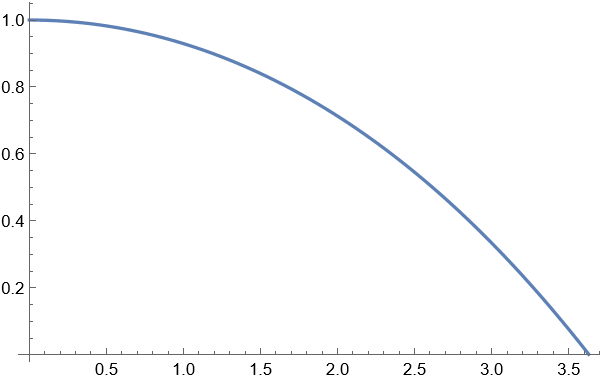
\includegraphics[scale=0.65]{Figures/contour-curve.png}
    \caption{Contour $C_{\rho}$ with $\rho \approx 2.46879$, which passes through the simple pole $i$.}
    \label{fig:contour-curve}
\end{figure}
There exist better choices of interpolation nodes to prevent such a phenomenon. We will discuss this topic in Section~\ref{Sec: 2-Che-Int}. 

\subsection{Chebyshev Interpolation}
\label{Sec: 2-Che-Int}
The Chebyshev interpolation aims to minimize the bound of the interpolation error. The bound of $\omega(x)$ depends only on the choice of the nodes, so a natural question is: What kind of interpolation nodes will \emph{minimize} 
$\max_{x\in [a, b]} \prod_{j=0}^n |x-x_j|$. We first restrict our analysis to the interval $[a, b] = [-1,1]$ for simplicity, the general case will be discussed later.
 
\begin{example}
    When $n = 1$, $\omega(x) = (x - x_0)(x - x_1)$, this function changes sign over the subintervals $[-1, x_0)$, $(x_0, x_1)$, $(x_1, 1]$, then we can compute the maximum of $|\omega(x)|$ on these subintervals. Therefore, we need to solve 
    \begin{equation}
        \min_{x_0, x_1\in [-1,1]}\max((1 + x_0)(1 + x_1), \frac{(x_1-x_0)^2}{4}, (1 - x_0)(1 - x_1) ),
    \end{equation}
    while we can observe that 
    \begin{equation}
       \frac{1}{2} (1 + x_0)(1 + x_1) +  \frac{(x_1-x_0)^2}{4} + \frac{1}{2}(1 - x_0)(1 - x_1) = 1 + \frac{(x_0 + x_1)^2}{4}\ge 1
    \end{equation}
    holds for any choice of $x_0, x_1$, which means the maximum is at least $\sfrac{1}{2}$, it occurs when all terms are equal and $x_0 + x_1 = 0$. Hence $x_0 = -\sfrac{\sqrt{2}}{2}, x_1 = \sfrac{\sqrt{2}}{2}$.
\end{example}

\begin{definition}
    The Chebyshev polynomials of the first kind are defined by: 
    $$T_k(x) = \cos (k\arccos x),\quad x\in[-1,1].$$
\end{definition}
\begin{theorem}
\label{Thm: 2-Che-Pro}
    The Chebyshev polynomial satisfies the following: 
    \begin{enumerate}
        \item $T_k(\cos\theta) = \cos k\theta, \quad \theta\in [0, \pi]$.
        \item $T_0 \equiv 1$, $T_1(x) = x$ and 
        $$T_{k+1}(x) = 2 x T_{k}(x) - T_{k-1}(x), \quad k\ge 1.$$
        \item $\max_{x\in[-1,1]} |T_k(x)| = 1$.
        \item The leading coefficient of $T_k(x)$ is $2^{k-1}$.
        \item $T_k$ has a total of $(k+1)$ extrema $s_j = \cos(\frac{j\pi}{k}), j = 0, 1,\dots, n$ in the interval $[-1,1]$ such that $T_k(s_j) = (-1)^j$.
    \end{enumerate}
\end{theorem}
\begin{proof}
    The first three statements are straightforward after replacing the variable $x = \cos\theta$. The fourth statement is an immediate result, with induction through the recursion formula 
    $T_{k+1}(x) = 2 x T_k(x) - T_{k-1}$. The last statement is trivial.
\end{proof}
More importantly, the Chebyshev polynomial has the following optimality property. 
\begin{theorem}
\label{Thm: 2-Che-opt}
    The optimal choice of interpolation nodes $\{x_j\}_{j=0}^{n}$ that minimize $\max |\omega(x)|$ is the extrema of Chebyshev polynomial $T_{{n+1}}$.
    \begin{equation}\label{EQ: CHEBY}
        \min_{x_j\in[-1,1]} \max_{x\in[-1,1]} |\omega(x)| =   \max_{x\in[-1,1]} \frac{1}{2^n}|T_{n+1}(x)|  = \frac{1}{2^n}
    \end{equation}
\end{theorem}
\begin{proof}
    Let the roots of $T_{n+1}(x)$ be $z_0, z_1, \dots, z_{n}\in [-1, 1]$, then we can write 
    $$T_{n+1} = 2^{n}(x - z_0)(x-z_1)\dots (x - z_{n}),$$
    therefore $\frac{1}{2^n} T_{n+1}(x)$ is a polynomial with leading coefficient as $1$. Since $\max_{x\in[-1,1]} |T_{n+1}(x)| = 1$, it is clear that $\max_{x\in [-1,1]} \frac{1}{2^n}|T_{n+1}(x)| = \frac{1}{2^n}$, which is the second equality in~\eqref{EQ: CHEBY}. For the first equality, we try to prove it by contradiction. Let $x_0, x_1, \dots, x_n\in [-1, 1]$, such that 
    $$\max_{x\in[-1,1]}|\omega(x)| < \frac{1}{2^n},$$
    then we define the polynomial $\psi(x) = \frac{1}{2^n}T_{n+1}(x)- \omega(x)$, its degree is at most $n$ due to cancellation, therefore at most have $n$ zeros. On the other side, because $\frac{1}{2^n}T_{n+1}(s_j) = \frac{1}{2^n}(-1)^j$ achieves the extrema at $s_j = \cos(\frac{j\pi}{n+1})$, $j=0,\dots, (n+1)$, the polynomial $\psi(s_j)$ must share the same sign of $\frac{1}{2^n}T_{n+1}(s_j)$. This means $\psi(x)$ changes sign $(n+1)$ times, hence $(n+1)$ zeros. It is a contradiction.
\end{proof}
\begin{definition}
    The interpolation nodes $z_j = \cos(\frac{(2j+1)\pi}{2(n+1)})$, $j = 0, 1, \dots, n$ are called ``\textit{Chebyshev nodes}''. These nodes are the zeros of Chebyshev polynomial $T_{n+1}$.
\end{definition}
We can generalize the above theorem to any interval $[a, b]$. One can define the affine transformation $\phi$ mapping $[-1,1]$ to $[a, b]$ by $\phi(x) = \frac{1}{2} (a + b + (b-a)x)$. It is not difficult to prove the following.
\begin{corollary}
\label{Cor: 2-Che-err-any}
    The optimal choice of interpolation nodes that minimize $\max |\omega(x)|$ on $[a, b]$ are, $\phi(z_j)$ and 
   $$\min_{x_j\in [a, b]} \max_{x\in [a, b]} |\omega(x)| = \frac{(b-a)^{n+1}}{2\cdot 4^n}.$$
   This bound is much smaller than the bound for equally spaced nodes.
\end{corollary}

\subsection{Stability of Polynomial Interpolation}
\label{SSec: 2-Sta-Pol-Int}
Suppose there is some perturbation of the data $\tilde{y}_j = y_j + \eps_j$ at the interpolation node $x_j$. Let $\tilde{f}_n(x)$ and $f_n(x)$ be the interpolating polynomials on perturbed data and original data. Then, with Lagrange polynomials, 
\begin{equation}
    \begin{aligned}
        |f_n(x) - \tilde{f_n}(x)| &= |\sum_{j=0}^n (y_j - \tilde{y}_j) L_j(x)| \\
        &\le \left(\max_{j} |\eps_j|\right) \sum_{j=0}^n |L_j(x)|.
    \end{aligned}
\end{equation}
Here $\lambda_n(x) := \sum_{j=0}^n |L_j(x)|$ is the \emph{Lebesgue function}. It is a piecewise polynomial. Its maximum $\Lambda_n$ is the \emph{Lebesgue constant} and only depends on the choice of interpolation nodes. 
For the equally spaced nodes, this Lebesgue constant grows exponentially. In fact,~\cite{turetskii1940bounding} proved the following sharp result. 
\begin{lemma}
    \label{Lem: 2-Leb-Con}
    Let $\{x_j\}_{j=0}^n$ be equispaced nodes on $[0, 1]$, then the Lebesgue constant 
    \begin{equation}
      \Lambda_n  =  \frac{2^{n+1}}{e n \log n} \left(1 + o(1)\right), \quad n\to\infty. 
    \end{equation}
\end{lemma}
\begin{proof}
    Assume $n\ge 3$, we prove the lower bound by construction. Let $f(x) = e^{i n\pi x}$ and define $p_n(x) = \sum_{j=0}^{n} f(x_j) L_j(x)$ as the interpolation polynomial at nodes $x_j = j \Delta$, $\Delta = \sfrac{1}{n}$, then $$|p_n(x)| = \left| \sum_{j=0}^{n} (-1)^j L_j(x) \right| \le \Lambda_n.$$
    Let $\delta_{+}$ be the forward difference operator
    \begin{equation}
       \delta_{+} p_n(x) := p_n(x+\sfrac{1}{n}) - p_n(x),
    \end{equation}
    then $ p_n(x_j) =  (1+\delta_{+})^j p_n(0)$ for $j=0,1,\cdots, n$, which means the interpolation polynomial is
    \begin{equation}
    \label{EQ: NEWTON-FORM-EQUI}
       p_n(x) = \sum_{k=0}^n \binom{nx}{k} \delta_+^k p_n(0) = \sum_{k=0}^n \binom{nx}{k} \delta_+^k f(0),
    \end{equation}
    which is exactly the Newton form at the equispaced nodes. See Section~\ref{SSec: 2-New-For}. Because $\delta_+ f(x) = (e^{i\pi} - 1)f(x) = -2 f(x)$ acts as a multiplicative operator, therefore 
    \begin{equation}
        p_n(x) = \sum_{k=0}^n \binom{nx}{k}  (-2)^k.
    \end{equation}
    Let $x_{\ast} = \frac{1}{n \log n}$ and set $\mu = n x_{\ast}\in(0, \sfrac{1}{\log(3)})$. Then, for $k\ge 1$, we have 
    \begin{equation}
        \frac{ \binom{\mu}{k}  (-2)^k  }{ \binom{\mu}{k + 1}  (-2)^{k + 1} } = \frac{k+1}{2(k - \mu)} > \frac{1}{2}.
    \end{equation}
    Therefore, 
    \begin{equation}
    \begin{aligned}
         \Lambda_n &\ge  |p_n(x_{\ast})| \ge \binom{\mu}{n}  (-2)^n \left(2 - \frac{1}{2^n}\right) - 1 \\
         &=\exp\left( \log\mu - \log n + \sum_{k=1}^{n-1} \log\left(1 - \frac{\mu}{k}\right) \right) (2^{n+1} - 1) - 1.
    \end{aligned}
    \end{equation}
    Denote the positive constant $C = 2(1 - \sfrac{1}{\log(3)})$ and notice $\log(1 - x) \ge -x - \frac{x^2}{C}$ for all $x\in (0, \sfrac{1}{\log(3)})$, then 
    \begin{equation}
    \begin{aligned}
        \Lambda_n &\ge \frac{\mu}{n} \exp\left(- \mu\sum_{k=1}^{n-1}\frac{1}{k}\right) \exp\left(-\frac{\mu^2}{C} \sum_{k=1}^{n-1}\frac{1}{k^2}\right)(2^{n+1} - 1) - 1 \\
        & \ge \frac{\mu}{n} \exp(-\mu (\log n + \gamma))\exp\left(-\frac{\pi^2\mu^2}{6C}\right)(2^{n+1} - 1) - 1 \\
        & =\frac{2^{n+1}}{e n \log n} \left(1 + o(1)\right).
    \end{aligned}
    \end{equation}
    We notice that if $\|f\|_{\infty}\le 1$,  then $\|\delta_{+} f\|_{\infty}\le 2$, using~\eqref{EQ: NEWTON-FORM-EQUI}, the upper bound of $\Lambda_n$ can be estimated by
    \begin{equation}
        \Lambda_n \le \sup_{x\in (0, 1)}\sum_{k=0}^n \left|\binom{nx}{k}\right| 2^k.
    \end{equation}
    By symmetry, it is sufficient to consider $x\le \sfrac{1}{2}$, otherwise, a similar bound can be derived with the backward difference operator $\delta_{-}$. Hence, 
    \begin{equation}
    \begin{aligned}
        \Lambda_n &\le \sum_{k=0}^{\lceil \sfrac{n}{2} \rceil} \binom{\lceil \sfrac{n}{2} \rceil}{k} 2^k + \sup_{z\in (0, \sfrac{n}{2})}  \sum_{k=\lceil \sfrac{n}{2} \rceil + 1}^{n} \binom{z}{k} 2^k \\
        &= 3^{ \lceil \sfrac{n}{2} \rceil } + \sum_{k = \lceil\sfrac{n}{2} \rceil + 1}^n  \frac{2^k}{e k \log k}\left(1 + o(1)\right),
    \end{aligned}
    \end{equation}
    where the following inequalities are applied:  
    \begin{equation}
        \begin{aligned}
            &\left|\binom{z}{k}\right|\le \binom{\lceil \sfrac{n}{2} \rceil}{k},\quad \forall z,k\le \lceil \sfrac{n}{2} \rceil
        \end{aligned}
    \end{equation} 
    and $\forall k \ge \lceil\sfrac{n}{2} \rceil + 1$, 
    \begin{equation}
        \begin{aligned}
            \sup_{z\in (0, \sfrac{n}{2})}\left|\binom{z}{k}\right| &=  \sup_{z\in (0, \sfrac{n}{2})} \frac{\sin(\pi(z - l))}{\pi k!} \Gamma(z+1)\Gamma(k - z) \\
            &=\sup_{z\in (0, 1)} \frac{\sin(\pi(z - l))}{\pi k!} \Gamma(z+1)\Gamma(k - z) \quad (\text{by comparison})\\&\le \sup_{z\in (0, 1)}\frac{z}{k}\left(\frac{z+1}{k - z}\right)^z \quad (\text{by Gautschi's inequality})\\
            &= \frac{1}{e k \log k}\left(1 + o(1)\right).
        \end{aligned}
    \end{equation}
    Therefore,  
    \begin{equation}
        \Lambda_n \le 3^{\lceil \sfrac{n}{2}\rceil}+  \frac{1}{e \log n} \left( \sum_{k=\lceil \sfrac{n}{2}\rceil+1}^n \frac{2^k}{k}\right) (1 + o(1)) =  \frac{2^{n+1}}{e n \log n}  (1 + o(1)).
    \end{equation}
\end{proof}
For the general case, it has been proved by Paul Erd{\"{o}}s (1964) that for any set of interpolation nodes, 
\begin{equation}
    \Lambda_n > \frac{2}{\pi}\log(n+1) + \frac{1}{2},\quad  n\ge 0.
\end{equation}
As the number of nodes $n\to \infty$, $\Lambda_n \to \infty$. This leads to the result of Faber that, for any choice of nodes, there exists a continuous function not able to be approximated by the interpolating polynomial. The Chebyshev nodes are almost optimal, in the sense that 
\begin{equation}
    \Lambda_{n, \textrm{Chebyshev}} < \frac{2}{\pi}\log(n+1) + 1.
\end{equation}
The set of nodes that minimizes $\Lambda_n$ is difficult to compute. A slightly better set of nodes than Chebyshev nodes are the \emph{ extended Chebyshev nodes}:
\begin{equation}
    \tilde{x}_j = \frac{\cos\left(\frac{2j+1}{2(n+1)\pi}\right)}{\cos\left(\frac{\pi}{2(n+1)}\right)}.
\end{equation}
\subsection{Newton Form}
\label{SSec: 2-New-For}
The Newton form is useful when we dynamically add interpolation nodes. Consider the following scenario: we already have found an interpolation polynomial $f_k$ through the data $(x_0, y_0)$, $(x_1, y_1)$,$\dots$, $(x_k, y_k)$, then if an addition pair $(x_{k+1}, y_{k+1})$ is provided, how can we effectively transform $f_k$ to $f_{k+1}$? If we write, 
$$f_{k+1}(x) = f_k(x) + c_{k+1} (x - x_0)(x - x_1)\dots (x - x_{k}), $$
then $f_{k+1}(x_j) = f_k(x_j)$, $j = 0, 1,\dots, k$. Therefore, we only need to take care of the equality $f_{k+1}(x_{k+1}) = y_{k+1}$, which means that 
\begin{equation}\label{EQ: CK}
    c_{k+1} = \frac{y_{k+1} - f_k(x_{k+1})}{\prod_{j=0}^k (x_{k+1} - x_j)}.
\end{equation}
Such an inductive procedure produces the Newton form: 
\begin{equation}\label{EQ: NEWTON}
    f_n(x) = c_0 + c_1 ( x - x_0) + c_2 (x - x_0)(x - x_1)+\dots+c_{n}(x-x_0)\dots (x - x_{n-1}).
\end{equation}
where the constant $c_j$ depends on $x_0, x_1, \dots, x_{j}$ only. Polynomials $\prod_{j=0}^k (x - x_j)$ are called \emph{Newton polynomials}. When the coefficients $c_k$ are known, the Newton form~\eqref{EQ: NEWTON} can be evaluated by the famous ``Horner's scheme'' (see Exercise~\ref{Prb: 1-Theo-3}), which is
\begin{equation}\label{EQ: HORNER}
    f_n(x) = c_0 + (x-x_0)(c_1 + (x-x_1)(c_2 + (x-x_2)(c_3 + \dots))),
\end{equation}
the evaluation order starts from the innermost part $c_n (x -x_{n-1})$. This formulation has a complexity of $3n$ flops. 

\begin{remark}
    The computation of $c_k$ is not cheap from~\eqref{EQ: CK}. A naive algorithm with Horner's scheme roughly takes $\sfrac{5n^2}{2}+\cO(n)$ flops to compute all coefficients. The ``divided differences'' is a better way to compute $c_k$.
\end{remark}
\begin{definition}
    Let the interpolation nodes be $\{x_0, x_1, \dots, x_n\}$, the ``divided differences'' are defined recursively as follows (the square bracket is used to distinguish from the usual bracket): 
    \begin{equation}
        \begin{aligned}
            f[x_j] &:= f(x_j),\\
        f[x_{j}, \dots, x_{j+k}] &:= \frac{f[x_{j+1},\dots, x_{j+k}] - f[x_j,\dots, x_{j+k-1}]}{x_{j+k} - x_{j}},
        \end{aligned}
    \end{equation}
    where $0\le j, k\le n$ and $j+k\le n$.
\end{definition}
The following example graph helps to understand the relationships among the divided differences. 

\begin{tcolorbox}
    \begin{equation}\label{EQ: ALG NEWTON}
    \begin{aligned}
        f[x_0] &               &\\ 
               &\searrow       &\\ 
        f[x_1] &\to f[x_0, x_1]& \\
               &\searrow        &\searrow&\\ 
        f[x_2] & \to f[x_1, x_2]&\to& f[x_0, x_1, x_2]\\
               &\searrow        &\searrow& &\searrow&\\ 
        f[x_3] &\to f[x_2, x_3] &\to& f[x_1, x_2, x_3] &\to & f[x_0, x_1, x_2, x_3]\\
               &\searrow        &\searrow & &\searrow&  &\searrow &\\ 
        f[x_4] & \to f[x_3, x_4]&\to& f[x_2, x_3, x_4] &\to & f[x_1, x_2, x_3, x_4] &\to&  f[x_0, x_1, x_2, x_3, x_4] 
    \end{aligned}
\end{equation}
\end{tcolorbox}
Calculating all the divided differences requires $\sfrac{3n^2}{2} +\cO(n)$ flops. The following theorem is the main statement for the Newton form.
\begin{theorem}
\label{Thm: 2-New-for}
    The interpolation polynomial $f_n$ in Newton form is given by, 
    \begin{equation}
        f_n(x) = f[x_0] + f[x_0, x_1](x-x_0) + \dots + f[x_0, \dots, x_n](x - x_0)(x - x_1)\dots (x - x_{n-1}).
    \end{equation}
    In other words, $c_k = f[x_0, \dots, x_k]$.
\end{theorem}
\begin{proof}
    We prove this by induction. Assume that the statement is true for $n$ and the interpolation node and the corresponding values  $(x_i, f[x_i])$, $i=0,1,\dots, n$. For a new node and value $(x_{n+1}, f[x_{n+1}])$, it is known from~\eqref{EQ: CK} that $c_{n+1}$ is the coefficient of the leading power. Let $g_n$ be the interpolation polynomial in Newton form through nodes $(x_i, f[x_i])$, $i=1,2,\dots, n+1$, then 
    $$\psi(x)  := g_n(x)(x - x_0) - f_n(x)(x - x_{n+1})$$
    satisfies that $\psi(x_j) = f[x_j](x_{n+1} - x_0)$ for $0\le j\le {n+1}$. Therefore,
    \begin{equation}
        f_{n+1}(x) = \frac{g_n(x)(x - x_0) - f_n(x)(x - x_{n+1})}{x_{n+1} - x_0}.
    \end{equation}
    The leading power's coefficient is then 
    \begin{equation}
        \frac{f[x_1, \dots, x_{n+1}] - f[x_0, \dots, x_n]}{x_{n+1} - x_0} = f[x_0, x_1,\dots, x_{n+1}].
    \end{equation}
\end{proof}
\begin{remark}
    The divided difference $f[x_j, \dots, x_{j+k}]$ is the coefficient of leading power of the interpolating polynomial through $(x_j, f[x_j]), \dots, (x_{j+k}, f[x_{j+k}])$. It can be shown that 
    $$f[x_j, \dots, x_{j+k}] = \frac{1}{k!}f^{(k)}(\xi)$$
    for some $\xi\in [a, b]$. See Exercise~\ref{Prb: 2-Theo-4}.
\end{remark}
\begin{remark}
\label{Rem: 2-New-err}
    The error estimate can be derived by
    \begin{equation}
        f(x) - f_n(x) = f[x_0, x_1, \dots, x_n, x] (x-x_0)\dots (x - x_n).
    \end{equation}
\end{remark}
\begin{remark}
    The Newton form~\eqref{EQ: NEWTON} does not require distinct nodes. The divided difference can be defined as a limit for repeated nodes:
    \begin{equation}
        f[x_0, x_0] = \lim_{x_1 \to x_0} \frac{f[x_1] - f[x_0]}{x_1 - x_0} = f'(x_0).
    \end{equation}
    Moreover, using the Taylor expansion, $f[\underbrace{x_0,\dots, x_0}_{(k+1)\,\text{times}}] = \frac{1}{k!}f^{(k)}(x_0)$. However, the divided differences cannot be computed in such cases if the derivative values are not provided. We will discuss this scenario later in the Hermite interpolation polynomial; see Section~\ref{SSec: 2-Her-Pol-Int}.
\end{remark}
\begin{remark}
    The algorithm to compute the divided difference can be more efficient with a single column to store diagonal elements. $\leadsto$ represents the number that is not changing.
    \begin{tcolorbox}
        \begin{equation}
        \begin{aligned}
            \color{red}{f[x_0]} &    \leadsto  \color{green}{f[x_0]}          & \leadsto& \color{cyan}{f[x_0]} &\leadsto& \color{blue}{f[x_0]} &\leadsto& \color{black}{f[x_0]}\\ 
                   &\searrow       &\\ 
                   \color{red}{f[x_1]} &\to \color{green}{f[x_0, x_1]}&  \leadsto& \color{cyan}{f[x_0, x_1]}  &\leadsto& \color{blue}{f[x_0, x_1]} &\leadsto& \color{black}{f[x_0, x_1]}\\
                   &\searrow        &\searrow&\\ 
                   \color{red}{f[x_2]} & \to \color{green}{f[x_1, x_2]}&\to& \color{cyan}{f[x_0, x_1, x_2]} &\leadsto& \color{blue}{f[x_0, x_1, x_2]}&\leadsto& \color{black}{f[x_0, x_1, x_2]}\\
                   &\searrow        &\searrow& &\searrow&\\ 
                   \color{red}{f[x_3]} &\to \color{green}{f[x_2, x_3] }&\to& \color{cyan}{f[x_1, x_2, x_3]} &\to & \color{blue}{f[x_0, x_1, x_2, x_3]}&\leadsto& \color{black}{f[x_0, x_1, x_2, x_3]}\\
                   &\searrow        &\searrow & &\searrow&  &\searrow &\\ 
                   \color{red}{f[x_4]} & \to \color{green}{f[x_3, x_4]}&\to& \color{cyan}{f[x_2, x_3, x_4]} &\to & \color{blue}{f[x_1, x_2, x_3, x_4]} &\to&  f[x_0, x_1, x_2, x_3, x_4] 
        \end{aligned}
    \end{equation}
    \end{tcolorbox}
\end{remark}
% \subsection{Berstein Polynomial Interpolation}
% The Berstein basis polynomial is defined by 
% \begin{equation}
%     b_{\nu, n}(x) = \binom{n}{\nu} x^{\nu}(1-x)^{n-\nu},\quad  \nu = 0,\dots, n
% \end{equation}

\subsection{Hermite Polynomial Interpolation}
\label{SSec: 2-Her-Pol-Int}
The Lagrange polynomial interpolation only requires the values of the data function $h$ at each node. It can be generalized when the derivative values of $h$ are also available. 

Let the tuple $(h(x_j), h^{(1)}(x_j), \dots, h^{(m_j)}(x_j))$ be the provided derivative values at the interpolation node $x_j$, $j=0,\dots, n$ and $m_j\ge 0$. $N = \sum_{j=0}^n (m_j + 1)$ is the total number of constraints. It can be shown that there exists a unique polynomial $H_{N-1}\in \Pi_{N-1}$ satisfies 
$$H_{N-1}^{(k)}(x_j) = y_j^k:= h^{(k)}(x_j),\quad j=0,\dots, n,\quad 0\le k\le m_j.$$
This polynomial is called \emph{Hermite interpolation polynomial}. The idea to construct the Hermite interpolation polynomial borrows from the Lagrange polynomials, which is to find a basis $L_{jk}$ such that 
\begin{equation}\label{EQ: HERMITE CONSTRUCTION}
    \frac{d^p}{d x^p}L_{jk}(x_l) = \begin{cases}
        1, & l = j, k = p\\
        0, & \text{otherwise}.
    \end{cases}
\end{equation}
Once these polynomials are obtained, the Hermite interpolation is straightforward:
$$H_{N-1}(x) = \sum_{j=0}^n \sum_{k=0}^{m_j} y_j^k L_{jk}(x).$$
Its uniqueness can be concluded from the linear independence of the basis $L_{jk}$. However, the construction method in~\eqref{EQ: HERMITE CONSTRUCTION} is not the simplest. It is known that the Newton form~\eqref{EQ: NEWTON} works for repeated nodes as long as the diagram's diagonal~\eqref{EQ: ALG NEWTON} can be filled. Therefore, we can arrange the nodes 
$$\underbrace{x_0,\dots, x_0}_{(m_0+1)\,\text{times}}, \quad \underbrace{x_1,\dots, x_1}_{(m_1+1)\,\text{times}}, \quad \dots,\quad  \underbrace{x_n,\dots, x_n}_{(m_n+1)\,\text{times}}$$
In this way, all the necessary divided differences can be computed.
\begin{remark}
    The error estimate for Hermite polynomial interpolation will be the same as the Newton form, see Remark~\ref{Rem: 2-New-err}.
\end{remark}


\section{Trigonometric Interpolation}
\label{Sec: 2-Tri-Int}
Periodic functions occur in many applications, that is, $f(x + T) = f(x)$, $x\in \bbR$ for some $T > 0$. For example, a closed planar curve can be parameterized as a periodic function naturally. The polynomial interpolation does not suit periodic functions, this is because polynomials will eventually go to infinity as $x\to\infty$. The most used interpolation for the periodic function is the \emph{trigonometric polynomial interpolation}. In the following, we assume the period $T = 2\pi$ without loss of generality.



\subsection{Fourier Series}
\label{SSec: 2-Fou-Ser}
\begin{definition}
    For $n\ge 0$, we defined $F_n$ the space of trigonometric polynomials 
    \begin{equation}
        F_n := \{f(x) \mid f(x) = \frac{a_0}{2} + \sum_{k=1}^n a_k \cos kx + \sum_{k=1}^n b_k \sin kx,\; a_k, b_k\in\bbR\}.
    \end{equation}
    The coefficients $a_0,\dots, a_n$, $b_1,\dots, b_n$ can be also chosen as complex numbers. $f\in F_n$ is said to be of degree $n$ if $|a_n| + |b_n| > 0$.
\end{definition}
The concept of ``degree'' here can be validated by the addition theorem of trigonometric functions. For instance, if $f_1\in F_k$, $f_2\in F_l$, then $f_1 f_2 \in F_{k+l}$. In the next, we discuss the uniqueness of the interpolation with the trigonometric polynomial.
\begin{lemma}
\label{Lem: 2-Tri-pl-zer}
    A trigonometric polynomial $f\in F_n$ that has more than $2n$ zeros in $[0, 2\pi)$ must vanish identically.
\end{lemma}
\begin{proof}
    Rewrite the trigonometric function in the form of 
    \begin{equation}\label{EQ: COMPLEX}
        f_n(x) = \sum_{k=-n}^{n} \gamma_k e^{ik x}. 
    \end{equation}
    where $\gamma_0 = \frac{1}{2}a_0$ and $\gamma_{k} = \frac{1}{2}(a_k - ib_k)$ and $\gamma_{-k} = \frac{1}{2}(a_k + i b_k)$, $k=1,\dots, n$. Then substitute $z = e^{ix}$ and set 
    \begin{eqnarray}
        p(z) = \sum_{k = -n}^n \gamma_k z^{n + k}, 
    \end{eqnarray}
    one can rewrite $f_n(x) = z^{-n} p(z)$. If $f_n(x)$ has more than $2n$ zeros, then $p(z)$ has more than $2n$ zeros, which is a contradiction since $p(z)$ is a polynomial of degree $2n$.
\end{proof}
\begin{remark}
    Since $\sin nx\in F_n$ has $2n$ zeros $\frac{\pi j}{n}$, $j=0,\dots, 2n-1$, it means to uniquely determine a trigonometric polynomial in $F_n$, exactly $2n+1$ values are needed. This is also known as the ``Nyquist-Shanon sampling theorem''.
\end{remark}
A direct corollary is the linear independence of the functions $1$, $\cos k x$ and $\sin k x$, $k = 1, \dots n$, these $(2n+1)$ functions form a natural basis for the trigonometric polynomial space $F_n$. 
\begin{corollary}
\label{Cor: 2-Fou-bas-ind}
    The functions $1, \cos kx, \sin kx$, $k=1,\dots, n$ are linearly independent on $C [0, 2\pi]$, hence $F_n$ is a $(2n+1)$ dimensional space.
\end{corollary}
To determine the coefficients $a_k, b_k$ from $(2n+1)$ data pairs $(x_j, y_j)$, $j=0, \dots, 2n$. We follow the idea of Lagrange polynomials by creating the basis polynomial $l_k(x)$ such that
\begin{eqnarray}
    l_k(x_j) = \begin{cases}
        1, &j = k,\\
        0,&\text{otherwise}.
    \end{cases} 
\end{eqnarray}
\begin{remark}
    A natural idea is replacing $x - x_j$ in the Lagrange basis by $\sin(x - x_j)$ and produce something like 
$$\prod_{j=0, j\neq k}^{2n}\frac{\sin(x - x_j)}{\sin(x_k - x_j)}$$
but $\sin(x - x_j)$ has two roots on $[0, 2\pi)$, therefore we need to rescale it to $[0, \pi)$.
\end{remark}
\begin{theorem}
\label{Thm: 2-Tri-Lag}
    Let the basis trigonometric polynomial, 
    $$l_k(x) =\prod_{j=0, j\neq k}^{2n}\frac{\sin(\frac{x - x_j}{2})}{\sin(\frac{x_k - x_j}{2})} ,$$
    then the interpolation trigonometric polynomial is 
    \begin{eqnarray}
        f_n(x) = \sum_{k=0}^{2n} y_k l_k(x).
    \end{eqnarray}
\end{theorem}
\begin{proof}
    It remains to show $l_k\in F_n$. This can be seen by splitting $l_k$ into $n$ pairs, each pair takes the form of 
    \begin{eqnarray}
        \sin(\frac{x-x_0}{2})\sin(\frac{x-x_1}{2}) = \frac{1}{2}\cos\left( \frac{x_0 - x_1}{2}\right) - \frac{1}{2}\cos\left(\frac{2x - x_0 - x_1}{2}\right)\in F_1.
    \end{eqnarray}
\end{proof}
Computationally, we can reuse the previously known barycentric form, but there exist better methods. For simplicity, we consider the equal space nodes in the following (non-uniform nodes could achieve the same complexity though). 
\begin{eqnarray}
    x_j = \frac{2\pi j}{2n + 1}, \quad j = 0, \dots, 2n. 
\end{eqnarray}
We will try to locate the coefficients $\gamma_k$ in the complex form (see~\eqref{EQ: COMPLEX}) from the interpolation conditions.
\begin{equation}
    f_n(x_j) = y_j = \sum_{k=-n}^n \gamma_k e^{i k x_j}.
\end{equation}
Use the property of the functions $e^{ikx_j}$ that 
\begin{equation}
    \sum_{k=0}^{2n} e^{ik x_j} = \begin{cases}
        2n+1, & k = 0\\
        0, &\text{otherwise}.
    \end{cases}
\end{equation}
It is not difficult to derive 
\begin{equation}
    \sum_{j = 0}^{2n} y_j e^{-im x_j} = \sum_{k=-n}^{n} \gamma_k \sum_{j=0}^{2n} e^{i (k - m) x_j} = \gamma_{m} (2n+1).  
\end{equation}
Therefore, we can compute 
\begin{equation}\label{EQ: GAMMA}
    \gamma_m = \frac{1}{2n+1}  \sum_{j = 0}^{2n} y_j e^{-im x_j}.
\end{equation}
When the coefficients $\gamma_m$ are known, Horner's scheme can be employed to evaluate the trigonometric polynomial in $\cO(n)$ time complexity.  However, naive computing of all the coefficients $\gamma_k$ will cost $\cO(n^2)$ flops. The fast Fourier transform can reduce the time complexity to $\cO(n\log n)$.
\begin{remark}
    For an even number of equally spaced nodes $x_j = \frac{j\pi}{n}$, $0\le j\le 2n-1$, the basis $\sin( n x)$ equals to zero constantly. There are $2n$ coefficients to be determined only. We can derive a similar formula as~\eqref{EQ: GAMMA} by replacing $(2n+1)$ with $2n$.
\end{remark}

\subsection{Fast Fourier Transform}
\label{SSec: 2-Fas-Fou-Tra}
The discrete Fourier transform $\textup{\texttt{DFT}}$ of a vector $\ba = (a_0, \dots, a_{n-1})$ is to evaluate the following vector:
$$\textup{\texttt{DFT}}(\ba)_{k} := \frac{1}{n}\sum_{j=0}^{n-1} a_je^{-2\pi i jk/n},\quad k = 0,\dots, n-1.$$
This is the exact formula to compute the coefficients for the trigonometric interpolation polynomial. Such transform is most efficiently calculated through the fast Fourier transform (\texttt{fft}).
The fast Fourier transform exploits the symmetry in $e^{2\pi i j/n}$ when $n$ is the power of two using divide-and-conquer. Let $\omega = e^{-2\pi i/n}$ and define $c_k$ as 
\begin{equation}
    c_k = \frac{1}{n}\sum_{j=0}^{n-1} y_j\omega^{jk},\quad k = 0,\dots, n-1.
\end{equation}
Let $m = \sfrac{n}{2}\in \bbN$, then $\omega^n = 1$, $\omega^m = -1$. We can separate $c_k$ into two parts with even $j$ and odd $j$.
\begin{equation}\label{EQ: C_K}
    c_k = \frac{1}{2} A_k + \frac{1}{2} B_k \omega^k,\quad c_{k+m} = \frac{1}{2} A_k - \frac{1}{2} B_k \omega^k 
\end{equation}
where 
\begin{equation}\label{EQ: AK BK}
    \begin{aligned}
        A_k = \frac{1}{m} \sum_{j=0}^{m-1} y_{2j} (\omega^2)^{jk},\quad B_k = \frac{1}{m} \sum_{j=0}^{m-1} y_{2j+1} (\omega^2)^{jk},
    \end{aligned}
\end{equation}
both $A_k$ and $B_k$ are in the same form and similar to $c_k$, but with only half of the terms in summation. This implies a recursive algorithm. Suppose $A_k$ and $B_k$, $0\le k\le m-1$ can be computed with $f(m)$ operations each, then 
\begin{equation}
   f(n) =  f(2m) = 2 f(m) + 4m
\end{equation}
The second term includes $2m$ multiplications and $2m$ additions in~\eqref{EQ: C_K}. Therefore,
\begin{equation}
    \begin{aligned}
        f(n)& = 2f(\frac{n}{2}) + 2n \\
&= 4f(\frac{n}{4}) + 2 n + 2n \\ 
&=\dots \\
&= n f(1) + \underbrace{2n + \dots + 2n}_{\log_2 n \text{ times}} = 2n \log_2 n.
    \end{aligned}
\end{equation}
since $f(1) = 0$, no computation is needed in this case.  The \texttt{fft} is usually a standard routine in modern scientific computing software. 

\subsection{Interpolation Error of Trigonometric Polynomial}
\label{SSec: 2-Int-Err-Tri-Pol}
The $L^2$ error estimate will be discussed at a later point. This part only focuses on the $L^{\infty}$ error estimate. We will need the following lemma, the proof is left as an exercise (see Exercise~\ref{Prb: 2-Theo-6}).
\begin{lemma}
\label{Lem: 2-Dir-Ker}
    Let $g(x)$ be the truncated Fourier series of $f(x)$
     $$g(x) = \sum_{s = -n}^n \gamma_s e^{is x},\quad \gamma_s = \frac{1}{2\pi}\int_{0}^{2\pi} f(x) e^{-isx} dx$$
     then 
     \begin{equation}
         g(x) =\frac{1}{2\pi}  \int_{0}^{2\pi} D_n(x - y) f(y)   d y, 
     \end{equation}
     where $D_n(x)$ is the \emph{Dirichlet kernel}
     \begin{equation}
         D_n(x):=  \sum_{s=-n}^{n} e^{is x} = \frac{\sin((2n+1)x/2)}{\sin(x/2)}.
     \end{equation}
\end{lemma}
\begin{theorem}[Uniform convergence for H\"older continuous functions]
\label{Thm: 2-Uni-Conv-C2}
    If $f\in C^{0,\alpha}(\bbR)$ is a $2\pi$-period function, then the trigonometric interpolation polynomial with $2n+1$ equally spaced nodes converges uniformly as the number of nodes tends to infinity.
\end{theorem}
\begin{proof}
    Since $f\in C^{0,\alpha}(\bbR)$, there exists a constant $K > 0$ that $|f(x) - f(y) |\le K |x - y|^{\alpha}$. Let $g(x)$ be the truncated Fourier series
    $$g(x) = \sum_{s = -n}^n \gamma_s e^{is x},\quad \gamma_s = \frac{1}{2\pi}\int_{0}^{2\pi} f(x) e^{-isx} dx$$
   and denote $h(x) = f(x)- g(x) = \sum_{|s| > n} \gamma_s e^{isx}$ the reminder. The interpolation polynomial satisfies
    \begin{equation}
        \begin{aligned}
            f_n(x)& = \sum_{m=-n}^n \left(\frac{1}{2n+1}\sum_{j=0}^{2n} y_j e^{-im x_j}\right) e^{im x}  \\
             &=\sum_{m=-n}^n \left(\frac{1}{2n+1}\sum_{j=0}^{2n} ( g(x_j) + h(x_j) ) e^{-im x_j}\right) e^{im x} \\
             &= \sum_{m=-n}^n \left(\frac{1}{2n+1}\sum_{j=0}^{2n} ( \sum_{s = -n}^n \gamma_s  e^{is x_j }+ h(x_j) ) e^{-im x_j}\right) e^{im x} \\
             &=g(x)+ \sum_{m=-n}^n \left(\frac{1}{2n+1}\sum_{j=0}^{2n} h(x_j) e^{-im x_j}\right)e^{im x} \\
             &=g(x)+ \frac{1}{2n+1} \sum_{j=0}^{2n} h(x_j) \frac{\sin((2n+1)(x-x_j)/2)}{\sin((x-x_j)/2)}
        \end{aligned}
    \end{equation}
    Therefore,
    \begin{equation}\label{EQ: DIFF}
        |f - f_n| \le \|h\|_{\infty} \left( 1 + \frac{1}{2n+1} \sum_{j=0}^{2n} \left|\frac{\sin((2n+1)(x-x_j)/2)}{\sin((x-x_j)/2)}\right|\right).
    \end{equation}
    We first estimate 
    $$\sum_{j=0}^{2n} \left|\frac{\sin((2n+1)(x-x_j)/2)}{\sin((x-x_j)/2)}\right|$$
    Separate the nodes into two groups: The first group with $|x - x_j| < \frac{2\pi}{2n+1}$, the absolute value is bounded by $(2n+1)$, there are at most $3$ nodes lying in this region, thus the contribution of the first group is at most $\cO(n)$. The second group is $\pi\ge |x - x_j| \ge \frac{2\pi}{2n+1}$, and then one can estimate 
    \begin{equation}
        \left|\frac{\sin((2n+1)(x-x_j)/2)}{\sin((x-x_j)/2)}\right| \le \frac{\pi}{|x - x_j|},
    \end{equation}
    since $\pi \sin x \ge 2x $ for $0\le x\le \sfrac{\pi}{2}$. This implies the contribution from the second group is $\cO(n\log n)$, and the total contribution is bounded by $\cO(n\log n)$. Then~\eqref{EQ: DIFF} can be bounded by 
    \begin{equation}
        |f - f_n| \le C \|h\|_{\infty} \log n,
    \end{equation}
    where $C$ is an absolute constant. Next, we estimate $\|h\|_{\infty}$. Using Lemma~\ref{Lem: 2-Dir-Ker}, we can represent
    \begin{equation}
    \begin{aligned}
        h(x) &= \frac{1}{2\pi} \int_{-\pi}^{\pi} D_n(y) (f(x) - f(x - y) ) dy \\
        &= \frac{1}{2\pi} \sum_{k=-n}^{n} \int_{\frac{(2k-1)\pi}{2n+1}}^{\frac{(2k+1)\pi}{2n+1}} \frac{\sin((2n+1) y/2)}{\sin(y/2)}  (f(x) - f(x - y) ) dy.
    \end{aligned}
    \end{equation}
    Notice the cancellation property
    \begin{equation}
         \int_{\frac{(2k-1)\pi}{2n+1}}^{\frac{(2k+1)\pi}{2n+1}} \sin\left(\frac{(2n+1) y}{2}\right) dy = 0,
    \end{equation}
    then for any $y'\in \cI_k:= \left(\frac{(2k-1)\pi}{2n+1}, \frac{(2k+1)\pi}{2n+1}\right)$, we have 
    \begin{equation}
    \label{EQ: CANCELLATION F}
    \begin{aligned}
    &\left| \int_{\frac{(2k-1)\pi}{2n+1}}^{\frac{(2k+1)\pi}{2n+1}} \frac{\sin((2n+1) y/2)}{\sin(y/2)}  (f(x) - f(x - y) ) dy \right| \\
    &= \left| \int_{\frac{(2k-1)\pi}{2n+1}}^{\frac{(2k+1)\pi}{2n+1}} \sin((2n+1) y/2)  \left( \frac{(f(x) - f(x - y) )}{\sin(y/2)} - \frac{(f(x) - f(x - y') )}{\sin(y'/2)} \right) dy \right| \\
    &\le \frac{4}{2n+1}\sup_{y,y'\in \cI_k} \left| \frac{(f(x) - f(x - y) )}{\sin(y/2)} - \frac{(f(x) - f(x - y') )}{\sin(y'/2)} \right|\\
    &\le \frac{4K}{2n+1}\left(\frac{\frac{\pi}{2n+1}\left|\frac{(2|k|+1)\pi}{2n+1}\right|^{\alpha}+ \frac{(2|k|+1)\pi}{4n+2}\left|\frac{2\pi}{2n+1}\right|^{\alpha}}{\left|\frac{(2|k|-1)\pi}{4n+2}\right|^2}\right)\\
    &=\frac{8K\pi^{\alpha-1}}{(2n+1)^{\alpha}} \left( \frac{2(2|k|+1)^{\alpha}}{(2|k|-1)^2}+ 2^{\alpha}\frac{2|k|+1}{(2|k|-1)^2} \right),
    \end{aligned}
    \end{equation}
    Because $\left|\frac{2|k|-1}{2|k|+1}\right|\ge \frac{1}{3}$ for all $k\in\bbN$, we obtain the bound for $h$:
    \begin{equation}
    \begin{aligned}
        |h(x)| &\le  \frac{4K\pi^{\alpha-2}}{(2n+1)^{\alpha}} \sum_{k=-n}^{n}  \left( \frac{2(2|k|+1)^{\alpha}}{(2|k|-1)^2}+ 2^{\alpha}\frac{2|k|+1}{(2|k|-1)^2} \right)\\&
        \le  \frac{36K\pi^{\alpha-2}}{(2n+1)^{\alpha}} \sum_{k=-n}^{n}  \left( \frac{2}{(2|k|+1)^{2-\alpha}}+ \frac{ 2^{\alpha}}{(2|k|+1)} \right)\\
        &= \cO(n^{-\alpha} \log n).
    \end{aligned}
    \end{equation}
    Therefore $|f - f_n|=\cO( n^{-\alpha} |\log n|^2 )$.
\end{proof}
\begin{remark}
    The uniform convergence of trigonometric polynomial interpolation be further extended to general continuous functions with \emph{modulus of continuity} $\omega(f;\tau)$ satisfying $$\omega(f;\frac{1}{n})|\log n|^2 \to 0$$ as $n\to\infty$. The estimate of $\|h\|_{\infty}$ matches the work of Dunham Jackson (1913). More related topics are discussed in Chapter~\ref{Ch: 4-App}.
\end{remark}

\section{Spline Interpolation}
\label{Sec: 2-Spl-Int}
It has been seen that increasing the number of interpolation nodes will not always help improve the approximation. The spline interpolation is to conquer this issue by using the piecewise low-degree polynomials. 

\begin{definition}
    Let $x_0, \dots, x_n$ be the distinct nodes on $[a, b]$ such that $a = x_0 <\dots < x_n = b$. The piecewise defined function $s_k(x)$ on the interval $[a, b]$ is a spline of degree $k$ to the nodes if  
    \begin{equation}
        s_k|_{[x_j, x_{j+1}]} \in \Pi_k, \quad s_k\in C^{k-1}([a, b]).
    \end{equation}
    The spline function $s_k$ is $(k-1)$-times continuously differentiable and piecewise polynomial of degree $k$.
\end{definition}
Then the space of splines $s_k$ will be $(n + k)$ dimension: each interval has $(k+1)$ dimensions, each interface imposes $k$ constraints, therefore $n (k+ 1) - (n-1) k = n + k$ dimensions. This shows that to determine a spline on the nodes uniquely, we will require $n+1$ interpolation values and $k-1$ additional constraints. Usual choices are
\begin{enumerate}
    \item periodic splines. $s_k^{(m)}(a) = s_k^{(m)}(b)$ for $m = 0, 1, \dots, k-1$.
    \item natural splines. $s_k^{(l+j)}(a) = s_k^{(l+j)}(b) = 0$, $j = 0, 1,\dots, l-2$ and $k = 2l-1$ with $l\ge 2$.
\end{enumerate}
In the following, we discuss some useful examples of spline. 
\subsection{Linear Splines}
The linear splines are a special case of splines. It uses piecewise linear polynomials on each subinterval and does not impose any derivative continuity. Let $y_j$ be the interpolation values at nodes $x_j$, respectively. The interpolation has an explicit form:
\begin{equation}
    s_1(x) = y_{j-1} + \frac{x - x_{j-1}}{x_j - x_{j-1}} y_j
\end{equation}
on the interval $[x_{j-1}, x_j]$. It can be represented as a linear combination of the ``hat'' basis function $\theta_j(x)$, defined by
\begin{equation}
    \theta_j(x) = \begin{cases}
        \frac{x - x_{{j-1}}}{x_j - x_{j-1}}, & x\in [x_{j-1}, x_{j}],\quad 1\le j\le n\\
         \frac{x - x_{j+1}}{x_j - x_{j+1}}, & x\in [x_j, x_{j+1}],\quad 0\le j\le n-1\\
         0, & \text{otherwise}
    \end{cases}
\end{equation}
then $s_1(x)$ can be written as 
$$s_1(x) = \sum_{j=0}^n \theta_j(x) y_j.$$
The interpolation error can be derived directly from the previous theory for two interpolation nodes. Let $f\in C^2([a, b])$, then on $[x_{j-1}, x_j]$, the interpolation error is 
\begin{equation}
    \frac{1}{2!}f''(\xi) (x - x_{j-1})(x - x_j) \le \frac{1}{8} \|f''\|_{\infty} |x_j - x_{j-1}|^2.
\end{equation}
Therefore, the interpolation error on $[a, b]$ is $\frac{1}{8} \|f''\|_{\infty} h^2$, where $h = \max|x_j - x_{j-1}|$. Once $f''$ is not uniformly bounded or even $f'$ is not well-defined somewhere, e.g., $f\in C^{0,\alpha}[a, b]$, the interpolation error will be replaced by the modulus of continuity. On $x\in [x_j, x_{j+1}]$, we have 
\begin{equation}
\begin{aligned}
    |s_1(x) - f(x)| &= \left| \frac{ (x_{j+1} - x) y_j+ (x - x_j) y_{j+1}}{x_{j+1} - x_j} - f(x) \right| \\   
    &=  \left| \frac{ (x_{j+1} - x) (y_j - f(x)) + (x - x_j) (y_{j+1}-f(x))}{x_{j+1} - x_j}  \right| \\ &\le \omega(f; |x_{j+1} - x_j|),
\end{aligned}
\end{equation}
where $\omega(f;\tau)$ is the modulus of continuity of $f$.
\subsection{Cubic Splines}
The cubic splines are particularly important in practice. Let $a = x_0 < x_1 <\dots < x_n = b$, and the corresponding values are $y_j$, $j = 0, \dots, n$. The constraints for cubic splines are: piecewise polynomial of degree 3 and continuous second derivative.a Denote the interpolation spline as $s_3$, then $\dd{s_3}$ is a piecewise linear function. On the sub-interval $[x_{j-1}, x_j]$, it can be represented by 
\begin{equation}
    \dd{s_3}(x) = M_{j-1} \frac{x_j - x}{h_j} + M_j \frac{x - x_{j-1}}{h_j},\quad j = 1,\dots, n,
\end{equation}
where $h_j = x_j - x_{j-1}$, $M_j = \dd{s_3}(x_j)$. Integrating the above formula twice, 
\begin{equation}
    s_3(x) = M_{j-1} \frac{(x_j - x)^3}{6 h_j} + M_j \frac{(x - x_{j-1})^3}{6h_j} + A_j (x - x_{j-1}) + B_j
\end{equation}
The additional constants $A_j, B_j$ can be determined by imposing $f(x_{j-1}) = y_{j-1}$ and $f(x_j) = y_j$. That is 
\begin{equation}
    A_j = \frac{y_j - y_{j-1}}{h_j} - \frac{h_j}{6}(M_j - M_{j-1}),\quad 
    B_j = y_{j-1}-  M_{j-1} \frac{h_j^2}{6}.
\end{equation}
Now we will determine the constants $M_j$ using the first derivative's continuity. 
\begin{equation}
    s_3'(x_{j}^{-})  = s_3'(x_j^{+}), \quad j = 1,\dots, n-1.
\end{equation}
That is equivalent to $j=1,\dots, n-1$, 
\begin{equation}
\label{EQ: CUB-SPL-DER}
    \begin{aligned}
        s_3'(x_{j}^{-})  &= M_j\frac{h_j}{3} + M_{j-1}\frac{h_{j}}{6} + \frac{y_j - y_{j-1}}{h_j}  \\
        &= -M_j \frac{h_{j+1}}{3}  - M_{j+1}\frac{h_{j+1}}{6} + \frac{y_{j+1} - y_j}{h_{j+1}} = s_3'(x_j^{+}). 
    \end{aligned}
\end{equation}
We can write the corresponding equations into a tridiagonal linear system 
\begin{equation}
    \begin{pmatrix}
        \frac{h_1}{6} & \frac{h_1 + h_{2}}{3} & \frac{h_{2}}{6} & \\\\
        &\frac{h_2}{6} & \frac{h_2 + h_{3}}{3} & \frac{h_{3}}{6} & \\\\
        &&\ddots &  \ddots & \ddots & \\ \\
        &&& \frac{h_{n-1}}{6} & \frac{h_{n-1} + h_{n}}{3} & \frac{h_{n}}{6} &
    \end{pmatrix} \begin{pmatrix}
        M_0 \\\\M_1\\\\ \vdots\\\\ M_n
    \end{pmatrix} 
    = \begin{pmatrix}
        \frac{y_{2} - y_{1}}{h_{2}} - \frac{y_{1} - y_{0}}{h_1} \\\\
        \frac{y_{3} - y_{2}}{h_{3}} - \frac{y_{2} - y_{1}}{h_2} \\\\
        \vdots \\\\
        \frac{y_{n} - y_{n-1}}{h_{n}} - \frac{y_{n-1} - y_{n-2}}{h_{n-1}} 
    \end{pmatrix}
\end{equation}
In practice, the system will be rescaled for numerical stability. 
\begin{equation}\nonumber
    \begin{pmatrix}
        \frac{h_1}{2(h_1 + h_{2})} & 1 & \frac{h_{2}}{2(h_1 + h_{2})} & \\\\
        &\frac{h_2}{2(h_2 + h_{3})} & 1 & \frac{h_{3}}{2(h_2 + h_{3})} & \\\\
        &&\ddots &  \ddots & \ddots & \\ \\
        &&& \frac{h_{n-1}}{2(h_{n-1} + h_{n})} & 1 & \frac{h_{n}}{2(h_{n-1} + h_{n})} &
    \end{pmatrix} \begin{pmatrix}
        M_0 \\\\M_1\\\\ \vdots\\\\ M_n
    \end{pmatrix} 
    = \begin{pmatrix}
       d_1 \\\\
        d_2 \\\\
        \vdots \\\\
       d_{n-1}
    \end{pmatrix}
\end{equation}
where $d_j = \frac{3}{h_{j-1} + h_{j}}\left[ \frac{y_{j} - y_{j-1}}{h_{j}} - \frac{y_{j-1} - y_{j-2}}{h_{j-1}}\right]$. 
The above system still lacks 2 more constraints, since the matrix is of size $(n-1)\times (n+1)$. Then we can apply the periodic spline or natural spline conditions. For example, if the natural constraint is applied: $\dd{s_3}(a) = \dd{s_3}(b) = 0$. We should have two more equations: 
\begin{equation}
    M_{0} = M_{n} = 0.
\end{equation} 
Then we can simply ignore the first and last columns of the matrix (also $M_0$ and $M_n$). 
If the periodic constraint is imposed, then we can add two more constraints: $M_0 = M_{n}$ and 
$$-M_0 \frac{h_{1}}{3} - M_1 \frac{h_1}{6} + \frac{y_1 - y_0}{h_1} = M_n \frac{h_n}{3} + M_{n-1} \frac{h_n}{6} + \frac{y_n - y_{n-1}}{h_n}.$$
In both cases, the resulting linear system is still tridiagonal and the solution takes $\cO(n)$ time complexity with the Thomas algorithm. 

Another popular choice to complete the matrix is to impose the constraints in the similar form on $x_0$ and $x_n$: 
\begin{equation}
\label{EQ: EXTENSION}
    2M_0 + \frac{h_1}{h_0 + h_1} M_1 = d_0,\quad  \frac{h_n}{h_{n} + h_{n+1}} M_{n-1} + 2M_n = d_n,
\end{equation}
where $h_0 = h_{n+1} = 0$ and $d_0 = d_1$, $d_{n} = d_{n-1}$ are assumed. 
\begin{remark}
The Jacobi and Gauss-Seidel iterations are suitable for solving the system. The iteration will converge to system accuracy within $\cO(\log_2 \textup{u})$ iterations. Related topics are discussed in Chapter~\ref{Ch: 8-Mat-Com}.
\end{remark}
The error estimate for the cubic spline can be derived in a way similar to the Lagrange polynomial interpolation. The following result is attributed to Charles Hall (1968).
\begin{theorem}\label{THM: ERROR CUBIC SPLINE}
    Let $f\in C^4([a, b])$ and $a = x_0 < \dots < x_n = b$ be a set of nodes. Then the natural cubic spline $s_3$ interpolating $f$ satisfies 
    \begin{equation}
        \|f - s_3\|_{\infty} \le \frac{5}{384}\|f^{(4)}\|_{\infty} h^4,
    \end{equation}
    where $h = \max_j |x_j - x_{j-1}|$.
\end{theorem}
\begin{proof}
    Here we only state the rough idea to prove the error bound. Let $u(x)$ be the piecewise Hermite interpolation polynomial that 
    \begin{equation}
        u(x_j)=f(x_j), \quad u'(x_j) = f'(x_j),
    \end{equation}
    then one can estimate 
    \begin{equation}
        \max_{x\in [x_j, x_{j+1}]} |u-f|\le  \frac{1}{24}\|f^{(4)}\|_{\infty} (x - x_j)^2 (x - x_{j+1})^2 \le \frac{1}{384}\|f^{(4)}\|_{\infty} h^4.
    \end{equation}
    On the subinterval $[x_i, x_{i+1}]$, $s_3$ and $u$ are both cubic polynomial interpolations, thus 
    \begin{equation}
         u(x) - s_3(x) = \frac{(x - x_i)(x_{i+1} - x)}{(x_{i+1} - x_i)} \left( e'(x_i) \frac{x_{i+1} - x}{x_{i+1} - x_i}  - e'(x_{i+1})\frac{x - x_i}{x_{i+1} - x_i}\right), 
    \end{equation}
    where $e(x) = f(x) - s_3(x)$. 
    Therefore, 
    \begin{equation}
    \label{EQ: CUB-SPL-ERR-EST-KEY}
    \begin{aligned}
        \|f - s_3\|_{\infty} &\le  \|u - s_3\|_{\infty}  +  \|f - u\|_{\infty} \\
        &\le \frac{h}{4} \max_{0\le i\le n} |e'(x_i)| + \frac{1}{384}\|f^{(4)}\|_{\infty} h^4. 
    \end{aligned}
    \end{equation}
    Using~\eqref{EQ: CUB-SPL-DER}, we find that
\begin{equation}
    \frac{1}{h_j}\left[ 2 s'_3(x_j) + s'_3(x_{j-1}) \right] + \frac{1}{h_{j+1}}\left[2 s'_3(x_j) + s'_3(x_{j+1})\right] =\frac{3(y_j - y_{j-1})}{h_j^2} + \frac{3(y_{j+1} - y_j)}{h_{j+1}^2}, 
\end{equation}
Using Taylor expansion locally at $x_j$, there exist $\zeta\in (x_{j-1}, x_j)$ and $\xi\in (x_j, x_{j+1})$ that
\begin{equation}
    \frac{2 e'(x_j) + e'(x_{j-1})}{h_j} + \frac{2 e'(x_j) + e'(x_{j+1})}{h_{j+1}}= \frac{1}{24}\left[-h_j^2 f^{(4)}(\zeta)+ h_{j+1}^2 f^{(4)}(\xi)\right].
\end{equation}
Suppose 
$\max_{0 \le i\le n}|e'(x_i)|$ attains its maximum at node $x_{k}$, then 
\begin{equation}
    \left| \frac{2 e'(x_k) + e'(x_{k-1})}{h_j} + \frac{2 e'(x_k) + e'(x_{k+1})}{h_{k+1}} \right| \ge \frac{h_j+h_{j+1}}{h_j h_{j+1}} |e'(x_k)|.
\end{equation}
Therefore, by AM-GM inequality,
\begin{equation}
    \max_{0 \le i\le n}|e'(x_i)| \le \frac{h_{j}h_{j+1}}{24 (h_j + h_{j+1}) } (h_j^2 + h_{j+1}^2) \|f^{(4)}\|_{\infty} \le \frac{1}{24}h^3 \|f^{(4)}\|_{\infty}. 
\end{equation}
Finally, combined with the estimate~\eqref{EQ: CUB-SPL-ERR-EST-KEY} will arrive at the desired bound.
\end{proof}
\subsection{B-Spline Representation}
The definition of B-spline (short for basis spline) was initially proposed by~\cite{curry1947spline}. Let $\bt:= \{t_j\}_{j\in \cJ}$ be a nondecreasing sequence; the index set $\cJ$ consists of consecutive integers which may be finite or infinite. The sequence is called ``knots''. The B-splines are defined in the following recurrence relation. 
\begin{definition}[Cox–de Boor]
The B-splines of order one $B_{j, 1}$ consist of the characteristic functions of the knot intervals:
\begin{equation*}
    B_{j, 1}(x) = \begin{cases}
        1,\quad x\in [t_j, t_{j+1})\\
        0,\quad \text{ otherwise }
    \end{cases}
\end{equation*}
and for $k > 1$, the B-spline of order $k$ satisfies
    $$B_{j,k}(x) = \frac{x - t_j}{t_{j+k-1} - t_j} B_{j, k-1}(x) + \frac{t_{j+k} - x}{t_{j+k} - t_{j+1}} B_{j+1, k-1}(x).$$
\end{definition}
Using induction, we can show the following property of the B-spline (see Exercise~\ref{Prb: 2-B-SPL-NON-SUP}).
\begin{lemma}[Property I]
\label{Lem: 2-B-SPL-NON-SUP}
    Each spline $B_{j,k}$ is a non-negative piecewise polynomial of degree $k-1$ supported on $(t_j, t_{j+k})$.
\end{lemma}
\begin{lemma}[Property II]
\label{Lem: 2-B-SPL-PAR-UNI}
   For any order $k\ge 1$, the B-splines of order $k$ form a partition of unity:
   $$\sum_{j = 1}^n B_{j, k}(x) = 1,\quad x\in (t_{k}, t_{n+1}).$$
\end{lemma}
\begin{proof}
    Let us prove this by induction. For $k=1$, this is exactly the definition. Assume the conclusion for $k = l$, then for $x\in (t_{l+1}, t_{n+1})\subset (t_{l}, t_{n+1})$, since $(t_{l+1}, t_{n+1})\bigcap \supp B_{1, l} = \emptyset$ and $(t_{l+1}, t_{n+1}) \bigcap \supp B_{n+1, l} = \emptyset$, we have 
    \begin{equation}
    \begin{aligned}
        \sum_{j=1}^n B_{j, l+1}(x) &=   \sum_{j=1}^n  \frac{x - t_j}{t_{j+l} - t_j} B_{j, l}(x) +   \sum_{j=1}^n\frac{t_{j+l+1} - x}{t_{j+l+1} - t_{j+1}} B_{j+1, l}(x) \\
        &=  \sum_{j=1}^n  \frac{x - t_j}{t_{j+l} - t_j} B_{j, l}(x) +  \sum_{j=2}^{n+1} \frac{t_{j+l} - x}{t_{j+l} - t_{j}} B_{j, l}(x) \\
        &= \sum_{j = 1}^{n} B_{j, l}(x) - \frac{t_{l+1} - x}{t_{l+1} - t_1} B_{1, l}(x) +  \frac{t_{n+l +1} - x}{t_{n+l + 1} - t_{n+1}} B_{n+1, l}(x) \\
        &=1. 
    \end{aligned}
    \end{equation}
    As an extension of Lemma~\ref{Lem: 2-B-SPL-PAR-UNI}, we actually can show B-spline can represent any polynomials.
    \begin{lemma}[Marsden]
    For $k \ge 1$, the B-splines of order $k$ can represent the polynomial
    \begin{equation}
    \label{EQ: MARSDEN}
        (x - \mu)^{k-1} = \sum_{j=1}^n \phi_{jk}(\mu) B_{jk}(x),\quad x\in (t_{k}, t_{+1}), 
    \end{equation}
    where $\phi_{jk}(\mu) = \prod_{l=j+1}^{j+k-1} (t_{l} - \mu)$ if $k > 1$, otherwise $\phi_{jk}(\mu) = 1$.
    \end{lemma}
    \begin{proof}
    The equality can be proved by induction as well. For the induction step, by the recursive definition, we have
        \begin{equation}\nonumber
        \begin{aligned}
            \sum_{j=1}^n \phi_{j,l+1}(\mu) B_{j, l+1}(x) &= \sum_{j=1}^n  \frac{x - t_j}{t_{j+l} - t_j} \phi_{j,l+1}(\mu) B_{j, l}(x) +   \sum_{j=1}^n\frac{t_{j+l+1} - x}{t_{j+l+1} - t_{j+1}} \phi_{j,l+1}(\mu) B_{j+1, l}(x)\\
            &=  \sum_{j=1}^n  \frac{x - t_j}{t_{j+l} - t_j}(t_{j+l}-\mu) \phi_{j,l}(\mu) B_{j, l}(x) \\&\quad +  \sum_{j=2}^{n+1} \frac{t_{j+l} - x}{t_{j+l} - t_{j}} (t_{j-1+l}-\mu)\phi_{j-1, l}(\mu)  B_{j, l}(x) \\
            &=  \sum_{j=1}^n  \frac{x - t_j}{t_{j+l} - t_j}(t_{j+l}-\mu) \phi_{j,l}(\mu) B_{j, l}(x) \\&\quad +  \sum_{j=2}^{n+1} \frac{t_{j+l} - x}{t_{j+l} - t_{j}} (t_{j}-\mu)\phi_{j, l}(\mu)  B_{j, l}(x)\\
            &=  (x - \mu)  \sum_{j=1}^n\phi_{j,l}(\mu) B_{j, l}(x),\quad x\in (t_{l+1}, t_{n+1})\subset (t_{l}, t_{s+1}). 
        \end{aligned}
        \end{equation}
    \end{proof}
    The B-splines of order $k$ naturally define a linear subspace $\cS_{k,\bt}$:
    \begin{equation}
        \cS_{k,\bt} = \text{span} \left\{ B_{jk}(x) \mid j=1,\cdots, n\right\}.
    \end{equation}
    Then $\cS$ contains all polynomials of degree $\le k-1$. Indeed, differentiating~\eqref{EQ: MARSDEN} in $\mu$, one gets
    \begin{equation}
        \frac{(x - \mu)^{k - \nu}}{(k - \nu)!} = \sum_{j=1}^n\frac{(-1)^{\nu}\partial_{\mu}^{\nu} \phi_{jk}(\mu) B_{jk}(x)}{(k-1)!}, \quad x\in (t_{k}, t_{n+1}). 
    \end{equation}
    If a knot $t_i$ has a multiplicity of $m_i > 1$, that is, 
    $$t_{i-1} < \underbrace{t_i = t_{i+1} = \cdots = t_{i + m_{i} - 1} }_{\text{multiplicity } = m_i}< t_{i + m_i}, $$
    then let $\mu = t_i$, for any $1\le \nu \le m_i$, 
    \begin{equation}
        \frac{(x - t_i)^{k - \nu}}{(k - \nu)!} = \sum_{j= i - ( k -\nu)}^s \frac{(-1)^{\nu}\partial_{\mu}^{\nu} \phi_{jk}(t_i) B_{jk}(x)}{(k-1)!}, \quad x\in (t_{i + \nu-1}, t_{n+1}) = (t_i, t_{n+1}). 
    \end{equation}
    However, $\partial_{\mu}^{\nu} \phi_{jk}(t_i) = 0$ for $i-1 \ge j \ge i - (k-\nu)$, thus 
    \begin{equation}
         \frac{(x - t_i)^{k - \nu}}{(k - \nu)!} = \sum_{j= i}^n \frac{(-1)^{\nu}\partial_{\mu}^{\nu} \phi_{jk}(t_i) B_{jk}(x)}{(k-1)!}, \quad x\in (t_i, t_{n+1}). 
    \end{equation}
    We also notice $B_{jk}(x) = 0$ if $x\le t_i$ for all $j\ge i$, therefore, 
    \begin{equation}
        \frac{(x - t_i)^{k - \nu}_{+}}{(k - \nu)!} = \sum_{j= i}^n \frac{(-1)^{\nu}\partial_{\mu}^{\nu} \phi_{jk}(t_i) B_{jk}(x)}{(k-1)!}, \quad x\in (t_{k}, t_{n+1}).
    \end{equation}
    \end{proof}
    \begin{definition}
        Suppose $\bzeta = \{\zeta_i\}_{i=1}^{q+1}$ is an increasing sequence and denote by $\bm = \{m_i\}_{i=2}^q$ an integer nonnegative sequence that $m_i \le k$. Define $\Pi_{k, \bt, \bm}$ as the space of piecewise polynomials of degree at most $k-1$ with knots $\{\zeta_i\}_{i=1}^{q+1}$ and satisfying the additional jump condition $\forall f\in \Pi_{k, \bzeta, \bm}$ 
        \begin{equation}
            \partial^{\nu-1} f(\zeta_i^{+}) = \partial^{\nu-1} f(\zeta_i^{-}),\quad 1 \le \nu \le m_i.
        \end{equation}
    \end{definition}
    \begin{theorem}[Curry-Schoenberg]
        \label{Thm: 2-B-SPL-EQU-PP-SPA}
        Let the non-decreasing sequence $\bt$ be 
        \begin{equation}
            \underbrace{\zeta_1, \cdots, \zeta_1}_{\text{multiplicity } = k}, \underbrace{\zeta_2, \cdots, \zeta_2}_{\text{multiplicity } = k - m_2},\cdots, \underbrace{\zeta_{q}, \cdots, \zeta_q}_{\text{multiplicity } = k - m_n}, \underbrace{\zeta_{q+1}, \cdots, \zeta_{q+1}}_{\text{multiplicity } = k} 
        \end{equation}
        then on the interval $[t_{k}, t_{n+1}]$, $n = \text{card}(\bt) - k$, 
        $$\Pi_{k, \bzeta, \bm} = \cS_{k, \bt}.$$
    \end{theorem}
    \begin{proof}
        $\Pi_{k,\bzeta, \bm}$ is spanned by the basis functions 
        \begin{equation*}
            \begin{aligned}
                &(x - \mu)^{k-\nu}, \quad \nu = 1,\cdots, k; \\
                &(x - t_i)^{k - \nu}_{+},\quad i=2,\cdots, q,\quad 1\le \nu \le k - m_i.
            \end{aligned}
        \end{equation*}
       Therefore, $\Pi_{k,\bzeta, \bm}\subset \cS_{k, \bt}$. The dimension of $\cS_{k, \bt}$ is the number of B-splines $B_{jk}$, which is, $\text{card}(\bt) - k = q k - \sum_{i=2}^n m_i$ which corresponds to the total number of bases of $\Pi_{k,\bzeta, \bm}$. 
    \end{proof}
From now on, we assume the knot sequence $\bt$ is defined as Theorem~\ref{Thm: 2-B-SPL-EQU-PP-SPA}, where the first and last knots are repeated $k$ times, then the basic interval $[t_k, t_{n+1}]$ coincides with the range of knots. Using the partition of unity property, the spline function in $\cS_{k,\bt}$ is a strictly convex combination of the coefficients. In other words, the spline function is bounded from below and above by the coefficients nearby.
\begin{theorem}[Convex Hull]
    \label{Thm: 2-B-SPL-CON-NUM}
    Suppose $x \in (t_i, t_{i+1})$, then 
    $$ \min_{i+1-k\le j \le i} c_j \le  \sum_{j=i-k+1}^i c_j B_{jk}(x)  \le \max_{i+1-k\le j\le i} {c_j}.$$
\end{theorem}
\subsection{B-spline Interpolation}
\label{SSec: 2-B-SPL-INT}
Let $n = \dim(\cS_{k, \bt})$ for the knots $\bt$. For the observation data $\{(x_i, y_i)\}_{i=1}^n$, the B-spline interpolation finds a spline $f(x) = \sum_{j=1}^n c_j B_{jk}$ that 
\begin{equation}
    \sum_{j=1}^n c_j B_{jk}(x_i) = y_i, \quad i = 1,\cdots, n.
\end{equation}
We first carry out the criteria for existence and uniqueness for the interpolation.
\begin{theorem}[Existence and Uniqueness]
Let $\{x_j\}_{j=1}^n$ be strictly increasing. The matrix $A:= (B_{jk}(x_i))_{ij}$ is non-singular if and only if $B_{ik}(x_i) \neq 0$ or equivalently $t_i < x_i < t_{i+k}$.
\end{theorem}
\begin{proof}
    The ``only if'' part is trivial.
\end{proof}

\begin{theorem}[Well Conditioned]
    \label{Thm: 2-B-SPL-WEL-CON}
    Let $f = \sum_{j=1}^n c_j B_{jk}$ on $[t_k, t_{n+1}]$, then 
    \begin{equation}
        \frac{1}{D_{k,\infty}} \max_{1\le j\le n} |c_j| \le \|f\|_{\infty} \le \max_{1\le j \le n} |c_{j}|,
    \end{equation}
    where the condition number $D_{k,\infty} \le k 2^{k - 1}$. 
\end{theorem}
\begin{proof}
    
\end{proof}







\section{Reproducing Kernel Hilbert Space}
\label{Sec: 2-Rep-Ker-Hil-Spa}
Let $H$ be a Hilbert space of functions defined on $\cX$, with inner product $\aver{\cdot, \cdot}$ such that the \emph{point evaluation map} $x: H\mapsto \bbC$ is bounded $\forall x\in \cX$. Then $H$ is called \emph{reproducing kernel Hilbert space} or RKHS for short. By Riesz's representation Theorem, there exists $\psi_x\in H$ that 
\begin{equation}
    f(x) = \aver{f, \psi_x},\quad \forall f\in H.
\end{equation}
The function $\cK(x, y):=\psi_x(y)$ is the \emph{reproducing kernel}. 
\begin{example}
    $L^2[0, 1]$ with the usual inner product is not an RKHS. However, the Sobolev space $W^{1, 2}[0, 1]$ with its usual norm is a RKHS by the embedding theorems.
\end{example}
The kernel $\cK(x, y):\cX\times \cX\to\bbC$ satisfies 
\begin{equation}
    \cK(x, y) = \aver{\psi_x, \psi_y}, 
\end{equation}
and the kernel is Hermitian and positive definite. Its converse is also true.
\begin{theorem}[Moore-Aronszajn]
    \label{Thm: 2-MOO-ARO}
    If $\cK:\cX\times \cX\to\bbC$ is a Hermitian, positive definite kernel, then there is a unique RKHS with $\cK$ as its reproducing kernel.
\end{theorem}
\begin{proof}
    We prove the RKHS is $H=\overline{\text{span}\{\cK(x, \cdot) \mid x\in \cX\}}$ equipped with the induced inner product $\aver{\cK(x, \cdot), \cK(y,\cdot)}_H = k(x, y)$. The verification is straightforward. For uniqueness, let us assume $H'\supset H$ is another RKHS with kernel $\cK$ and inner product $\aver{\cdot, \cdot}_{H'}$. Then, 
    \begin{equation}
        \cK(x, y) = \aver{\cK(x, \cdot), \cK(y,\cdot)}_H = \aver{\cK(x, \cdot), \cK(y,\cdot)}_{H'},
    \end{equation}
    which implies the inner products are identical on $H$. Finally, $\forall f\in H'$, write $f = f_H + f_{H^{\perp}}$, then 
    \begin{equation}
        f(x) = \aver{f, \cK(x, \cdot)}_{H'} = \aver{f_H, \cK(x, \cdot)}_{H'}  + \aver{f_{H^\perp}, \cK(x, \cdot)}_{H'} = f_H(x).
    \end{equation}
    Therefore, $H' = H$.
\end{proof}
\subsection{Interpolation in RKHS}
Let $H$ be a RKHS with inner product $\aver{\cdot, \cdot}_H$. Suppose the data $\{(\ell_j, z_j)\}_{j=1}^m$ is generated by  $  z_j = \aver{\ell_j, f}_H $ such that  $\ell_j\in H^{\ast}$ and $f\in H$ is an \emph{unknown} function. The interpolation finds a function $f^{\ast}$ such that 
\begin{equation}
    \aver{\ell_j, f^{\ast}} = z_j,\quad j=1,\cdots, m.
\end{equation}

\section{Exercises}
The coding part and test cases are available on GitHub. 
\subsection{Theoretical Part}
\begin{problem}
    Prove Corollary~\ref{Cor: 2-Che-err-any}.
\end{problem}
\begin{problem}
    If $n$ is sufficiently large, prove the following bound instead for~\eqref{EQ: MAX-OMEGA}.
    \begin{equation}
        |\omega(x)|\le \prod_{j=0}^n |x - x_j| \le \frac{n!}{1 + \log n} \left|\frac{b-a}{n}\right|^{n+1}.
    \end{equation}
\end{problem}
\begin{problem}
\label{Prb: 2-Theo-2}
    Estimate the interpolation error for $e^x$ and $x^{-\sfrac{1}{2}}$ over the interval $[\frac{1}{2}, \frac{3}{2}]$ with equally spaced nodes and Chebyshev nodes, respectively.
\end{problem}
\begin{problem}
    Let $-1\le x_0 < x_1 <\dots < x_n \le 1$ be a set of interpolation nodes and $L_j(x)$ denotes the Lagrange basis polynomial at $x_j$. Prove if $x\in (x_i, x_{i+1})$, then 
    $$L_{i}(x) + L_{i+1}(x) \ge 1.$$
    Hint: Use Rolle's Theorem.
\end{problem}
\begin{problem}
    Prove the contour $C_{\rho}$ for Chebyshev nodes on $[-1, 1]$ is an ellipse with foci at $\pm 1$. 
\end{problem}
\begin{problem}
\label{Prb: 2-Theo-4}
    Let the nodes $x_0, \dots, x_n\in[a,b]$ and $f\in C^{n+1}([a, b])$. For any given $x\in[a, b]$, prove there exists $\xi\in [a, b]$ such that the divided difference $$f[x_0, x_1, \dots, x_n, x] = \frac{1}{(n+1)!}f^{(n+1)}(\xi).$$
    Hint: {Construct the interpolation polynomial on nodes $x_0, \dots, x_n$ with Newton form first, then regard $x$ as the additional node by~\eqref{EQ: NEWTON}, finally recall the Theorem~\ref{Thm: 2-Int-err}.}
\end{problem}
\begin{problem}
    Show that the divided difference $$f[x_0, x_1,\dots, x_n] = f[x_{\pi(0)}, x_{\pi(1)},\dots, x_{\pi(n)}],$$ where $\pi\in S_{n+1}$ is any permutation.
\end{problem}
\begin{problem}
\label{Prb: 2-Theo-6}
    Prove Lemma~\ref{Lem: 2-Dir-Ker}.
\end{problem}
\begin{problem}[discrete circular convolution]
    Let two vectors $\ba = (a_0,\dots, a_{N-1})$ and $\bb = (b_0, \dots, b_{N-1})$ and we assume the convention that $a_{N + j} = a_j$ and $b_{N+j} = b_j$ to extend the vector to infinite size. The discrete circular convolution $\bc = (c_0,\dots, c_{N-1}) = \ba\ast \bb$ is defined by 
$$c_j = \sum_{l = 0}^{N-1} a_l b_{j - l}.$$
Prove that 
$$\textup{\texttt{DFT}}(\bc) = \textup{\texttt{DFT}}(\ba)\circ \textup{\texttt{DFT}}(\bb),$$
where $\circ$ is the Hadamard product or element-wise product.
\end{problem}
\begin{problem}[Minimimum norm property] Let $f\in C^2([a, b])$ and $s_3$ be the \underline{natural} cubic spline with interpolating $f$. Prove 
    \begin{equation}
        \int_a^b |\dd{s_3}(x)|^2 dx \le \int_{a}^b |f''(x)|^2 dx 
    \end{equation}
    The equality holds only when $f(x) = s_3(x)$ everywhere.
    Hint: One needs to prove 
    \begin{equation}
        \int_a^b (f''(x) - \dd{s_3}(x)) \dd{s_3}(x) dx = 0,
    \end{equation}
    then simply use the AM-GM inequality. The above equality can be proved using integration-by-parts twice (remember the interpolation conditions).
\end{problem}
\begin{problem}
    Let the following tridiagonal matrix (corresponding to natural cubic spline)
    $$A = \begin{pmatrix}
        1 & \frac{h_{2}}{2(h_1 + h_{2})} & \\\\
        \frac{h_2}{2(h_2 + h_{3})} & 1 & \frac{h_{3}}{2(h_2 + h_{3})} & \\\\
        &\ddots &\ddots &  \ddots & \\ \\
        &&\ddots &\ddots &  \frac{h_{n-2}}{2(h_{n-2} + h_{n-1})} & \\ \\
        &&& \frac{h_{n-1}}{2(h_{n-1} + h_{n})} & 1&
    \end{pmatrix} $$
    and denote $B = A - I$. Prove $\|B\|_{\infty} \le \frac{1}{2}$ and $\|A^{-1}\|_{\infty}\le 2$. 
\end{problem}
\begin{problem}
\label{Prb: 2-B-SPL-NON-SUP}
    Prove the Lemma~\ref{Lem: 2-B-SPL-NON-SUP}.
\end{problem}
\subsection{Computational Part}
\begin{problem}
    Implement the divided difference to compute the coefficients of the Newton form. You should call the Horner's scheme from the previous coding project. State the consequence when the length of $[a, b]$ is very small. 
\end{problem}
\begin{problem}
    Implement the Lagrange interpolation schemes on equispaced and (extended) Chebyshev nodes.
\end{problem}
\begin{problem}
    Implement a routine to compute Hermite interpolation with $m_j = 1$ for each $j = 0, \dots, n$. Estimate your routine's time complexity and space complexity. 
\end{problem}
\begin{problem}
    Implement the cubic spline interpolation with periodic and natural spline conditions. 
\end{problem}

\begin{problem}
     Implement discrete Fourier transform using a recursive approach (assume the total number of nodes is a power of two).
\end{problem}

\begin{problem}
    Implement the B-splines $B_{jk}$ for the knots mentioned in Theorem~\ref{Thm: 2-B-SPL-EQU-PP-SPA}.
\end{problem}

% \bibliography{563}
\nocite{jackson1912approximation, jackson1913accuracy, erdHos1964problems,erdos1958problems,de1978practical,prenter2008splines,trefethen1991two}
\bibliographystyle{apalike}
\bibliography{chap2}

\chapter{Differentiation and Quadrature}
\label{Ch: 3-Dif-Qua}
A vast number of applications such as the calculation of tangent vectors or areas lead to the problem of computing 
\begin{equation}
    \cD(f) := \frac{d}{dx} f(x),\quad \cI(f) := \int_a^b f(x) dx, 
\end{equation}
for certain function $f(x)\in C^k([a, b])$. Accurate evaluations would sometimes be difficult if an analytic expression is absent. Especially when the function values of $f$ are only accessible at a finite number of nodes. Therefore, it is important to find simple yet effective methods to approximate the derivatives and integrals. 

\section{Extrapolation}
\label{Sec: 3-Ext}
From the previous discussion, we already know that interpolation provides an estimate \emph{within} the original observation range. The extrapolation is similar but aims to produce estimates outside the observation range. However, extrapolation may be subject to a greater uncertainty (Fig~\ref{FIG: EXTRAPO}), one should use it only when an overestimate is hardly occurring.
\begin{figure}[!htb]
    \centering
    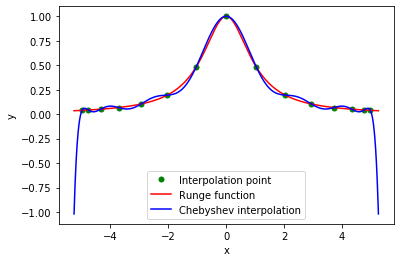
\includegraphics[scale=0.7]{extrapolate}
    \caption{Extrapolation behavior for Chebyshev interpolation with $15$ nodes.}
    \label{FIG: EXTRAPO}
\end{figure}

\subsection{Richardson Extrapolation}
\label{SSec: 3-Ric-Ext}
Suppose there is a sequence of estimates $A(h)$ depending on the parameter $h$ smoothly, the limit $A^{\ast} = \lim_{h\to 0^{+}} A(h)$ is the quantity to be computed. In practice, we only have access to $A(h)$ for a few values of $h$. Using these values to estimate $A^{\ast}$ is a typical problem in extrapolation. 

The basic idea behind \emph{Richardson extrapolation} is to use polynomial interpolation with a sequence of nodes $h_j\to 0$. Suppose that the function $A(h)$ admits the following asymptotic expansion:
\begin{equation}
    A(h) = a_0 + a_1 h^{\gamma} + a_2 h^{2\gamma} + \dots + a_k h^{k\gamma} + \cO(h^{(k+1)\gamma})
\end{equation}
for any $h > 0$ and $k\ge 0$. Then $A^{\ast} = a_0$ and $A(h) = A^{\ast} + \cO(h^{\gamma})$. Suppose we have access to the values $A(h_0),\dots, A(h_n)$, then this uniquely determines a polynomial $f_n\in\Pi_n$ and
$f_n(h_j^{\gamma}) = A(h_j)$. We will approximate $A(0)\approx f_n(0)$. The computation of $f_n$ follows the construction of Newton form. 
\begin{lemma}
\label{Lem: 3-Ric-Ext-Exp}
    Suppose $h_j$ can be represented as 
    $$h_j = \frac{\hbar}{t_j}$$
    for some adjustable parameter $\hbar$ and scaling constants $ 1 < t_0 < t_1<\dots < t_{n-1}$. Then 
    $$f_n(0) = A^{\ast} + (-1)^n \frac{a_{n+1}}{\prod_{j=0}^n t_j^{\gamma}} \hbar^{(n+1)\gamma} + \cO(\hbar^{(n+2)\gamma}),\quad \text{as }\hbar\to 0.$$
\end{lemma} 
\begin{proof}
    We view $A(h)$ as a polynomial with respect to $h^{\gamma}$ of degree $(n+1)$ with an addition perturbation $\cO(h^{(n+2)\gamma})$. Then we have the following. 
    \begin{equation}
        A(h) = p_{n+1}(h^{\gamma}) + \cO(h^{(n+2)\gamma}).
    \end{equation}
    Let $\tilde{f}_n$ be the interpolation polynomial of degree $n$ to $p_{n+1}$, 
    \begin{equation}
        p_{n+1}(x) \equiv \tilde{f}_n(x) + p[x, x_0, x_1, \dots, x_n] \prod_{j=0}(x - h_j^{\gamma}). 
    \end{equation}
    where $p[x, x_0, x_1, \dots, x_n]$ is the coefficient of the leading power in $p_{n+1}$, $a_{n+1}$. Thus, 
    \begin{equation}
        A^{\ast} = p_{n+1}(0) = \tilde{f}_n(0) +a_{n+1} \prod_{j=0}(0 - h_j^{\gamma}). 
    \end{equation} 
    Use the result we have discussed in the stability of polynomial interpolation, see Chapter~\ref{SSec: 2-Sta-Pol-Int}. Therefore, 
    \begin{equation}
        |\tilde{f}_n(0) - f_n(0)|\le \lambda_n(0) \cdot \cO(\hbar^{(n+2)\gamma})
    \end{equation}
    Here the Lebesgue function at zero $\lambda_n(0)$ is 
    \begin{equation}
        \lambda_n(0) = \sum_{j=0}^n \prod_{k=0, k\neq j}^n \left|\frac{h_k^{\gamma}}{h_k^{\gamma} - h_j^{\gamma}}\right| =  \sum_{j=0}^n \prod_{k=0, k\neq j}^n \left|\frac{1}{1 - (\frac{t_k}{t_j})^{\gamma}}\right|,
    \end{equation}
    which is independent of $\hbar$.
\end{proof}
The Richardson extrapolation considers the special choice of $t_j = t^j$ for some $t > 1$. The error estimate then is 
\begin{equation}
    f_n(0) = A^{\ast} + \left(\frac{(-1)^n}{t^{n(n+1)\gamma/2}} a_{n+1}\right) \hbar^{(n+1)\gamma} + \cO(\hbar^{(n+2)\gamma}).
\end{equation}
There are easier ways to calculate the Richardson extrapolation using the following expansion.
\begin{equation}
    A(h) - t^{\gamma} A\left(\frac{h}{t}\right) = (1 - t^{\gamma}) A^{\ast} + \cancel{a_1 \left(h^{\gamma} - t^{\gamma} \left(\frac{h}{t}\right)^{\gamma}\right)} + a_2\left(h^{2\gamma} - t^{\gamma}\left(\frac{h}{t}\right)^{2\gamma}\right) +\dots
\end{equation}
Let $A_1(h) = \frac{A(h) - t^{\gamma} A(\frac{h}{t}) }{1 - t^{\gamma}} $, we obtain the first iteration result as 
\begin{equation}
    A^{\ast} \approx A_1(h) + \cO(h^{2\gamma}),
\end{equation}
then follow the same idea, we cancel the $\cO(h^{2\gamma})$ term by
\begin{equation}
    A_1(h) - t^{2\gamma} A_1\left(\frac{h}{t^2}\right) = (1 - t^{2\gamma}) A^{\ast} + \cO(h^{3\gamma}).
\end{equation}
Therefore by taking $A_2(h) = \frac{A_1(h)- t^{2\gamma} A_1(\frac{h}{t^{2\gamma}})}{1 - t^{2\gamma}}$, the second iteration satisfies 
\begin{equation}
    A^{\ast}\approx A_2(h) + \cO(h^{3\gamma}).
\end{equation}
However, such a process can constantly refine the approximation due to the potentially fast-growing constant in the $\cO$ notation.

\subsection{Wynn's epsilon method}
\label{SSec: 3-Wynn-Eps-Met}
Wynn's $\eps$ method is another kind of extrapolation algorithm that is recommended as the best all-purpose acceleration method. It has a strong connection with Pad\'e approximation and continued fractions. We will not cover the detailed derivation of the theory in this section. However, Wynn's $\eps$ method still has its limitations if the sequence converges to the desired value too slowly. 

The algorithm is stated as follows. Let $s_0, s_1, \dots, s_n,\dots$ be a sequence converging to the desired quantity.
\begin{enumerate}
    \item Initialization. For $j = 0, 1, 2,\dots$, set 
    $$\eps_{-1}^{(j)} = 0 \text{ (guarding elements)}, \quad \eps_{0}^{(j)} = s_j.$$
    \item Iteration. For $j,k = 0,1,2,\dots$, 
    $$\eps_{k+1}^{(j)} = \eps_{k-1}^{(j+1)} + [\eps_{k}^{(j+1)} - \eps_{k}^{j}]^{-1}.$$
\end{enumerate}
The extrapolated results are stored at the columns $\eps_{2l}^{(j)}$, $j, l=0,1, \dots$.
\begin{example}
    It is known that $\sfrac{\pi}{4}$ can be calculated by the asymptotic expansion:
    \begin{equation}
        \arctan z = z - \frac{z^3}{3} + \frac{z^5}{5} - \dots 
    \end{equation}
    at $z = 1$. Define the function $A(h)$ such that 
    \begin{equation}
        A(h)= \sum_{j=0}^{1/h} \frac{(-1)^j}{2 j + 1} = \frac{\pi}{4} + a_1 h + a_3 h^3 + \dots
    \end{equation}
    Then the approximation error is $\cO(h)$, which is very slow. Taking $h=10^{-3}$ has around $2\times 10^{-4}$ error.  We test with two extrapolation algorithms.
    \begin{enumerate}
        \item [$\circ$] Richardson Extrapolation. We take $1/h = 250, 500, 1000, 2000$ and calculate that the Richardson extrapolation three times would result in almost machine precision.
        \item [$\circ$] Wynn's $\eps$ method. We take the sequence 
        $$s_k = \sum_{j=0}^k \frac{(-1)^j}{2 j + 1}$$
        as the truncated series at $z = 1$. With about 20 terms, we already reached machine precision.
    \end{enumerate}
\end{example}
\begin{theorem}
    TODO: Theory for $\eps$ method.
\end{theorem}
\section{Differentiation with Finite Difference}
Let $f\in C^2([a, b])$, we recall the Taylor expansion with reminder term, 
\begin{equation}
    f(x + h) = f(x) + h f'(x) + \frac{h^2}{2} f''(\xi),
\end{equation}
where $\xi = \xi(x)\in [a, b]$, therefore we can compute the derivative by 
\begin{equation}
    f'(x)  = \frac{f(x + h) - f(x)}{h} - \frac{h}{2} f''(\xi).
\end{equation}
This approximation offers a way to evaluate the derivative $f'(x)$ with the error term $\cO(h)$. In addition, the above formula is \emph{exact} when $f$ is a polynomial of degree $1$. We say that an approximation has degree $k$ accuracy if the approximation is \emph{exact} for any polynomial of degree $k$. 

Another important terminology is the \emph{order}. It describes the error term of the approximation. In the above case, the error term scales like $\cO(h)$ as $h\to 0$, then the approximation is of order $1$ or first order. In general, if the error term behaves like $\cO(h^p)$, then we can say that it is the $p$-th order approximation. 

The \emph{stencil} refers to a set of nodes used in the approximation. In the above example, we have used $x, x+h$. We can of course create its sibling
\begin{equation}
    f'(x) = \frac{f(x) - f(x - h)}{h} + \frac{h}{2} f''(\zeta),
\end{equation}
which uses the nodes $x-h, x$. When all nodes are $\ge x$ or $\le x$, we say the scheme is forward or backward, respectively.

\subsection{Finite Difference from Taylor Expansion}
All results related to finite difference can be easily derived from the Taylor expansion. Suppose we would like to approximate a high-order derivative $f^{(m)}(x)$ with some nodes scattered around $x$ in the following form. 
\begin{equation}
    \frac{1}{h^m} \sum_{j = 0}^n c_j f(x + a_j h) = f^{(m)}(x) + E(x, h),
\end{equation}
where $E$ is the error term and $a_j\in\bbZ$ (sometimes half integers are used). Since $h\to 0$, we can expand all $f(x + a_j h)$ locally by Taylor series and truncate at least order $(m+1)$.
\begin{equation}
    \frac{1}{h^m} \sum_{j=0}^n c_j \left( \sum_{p=0}^{m} \frac{1}{p!}f^{(p)}(x) a_j^p h^p + \frac{f^{(p+1)}(\xi_j)}{(p+1)!} a_j^{p+1} h^{p+1}\right).
\end{equation} 
We need all lower (and maybe higher than $m$-th) order derivatives of $f$ canceled in the above summation, which is (using Kronecker delta),
\begin{equation}
    \begin{aligned}
        \sum_{j=0}^n c_j a_j^p &= {m!} \cdot \delta_{pm}, \quad 0\le p \le m.
    \end{aligned}
\end{equation}
It is straightforward that $n \ge m$ is necessary; otherwise, the first equation system (Vandermonde matrix) must have a zero solution.  Suppose that we have found a solution $(c_j, a_j)$, $j=0,\dots, n$,  to the above system, then in the sequel, we try to estimate the error term $E(x, h)$. Especially, when $n = m$, there are two cases. Let the constant $C =  \sum_{j=0}^n c_j a_j^{m+1}$, then  
\begin{enumerate}
    \item If $C = 0$, then the error term can be estimated by expanding to $(m+2)$-th derivative. 
    \begin{equation}\label{EQ: ERROR FD}
        E(x, h) = \frac{1}{h^m}\sum_{j=0}^n c_j \frac{f^{(m+2)}(\xi_j)}{(m+2)!} a_j^{m+2} h^{m+2} = h^2 \left(\sum_{j=0}^n c_j  a_j^{m+2}\frac{f^{(m+2)}(\xi_j)}{(m+2)!}\right)\,.
    \end{equation}
    One can expect higher-order accuracy when more terms are involved. 
    \item If $C\neq 0$, then the error term is 
    \begin{equation}\label{EQ: ERROR FD NZERO}
        E(x, h) = \frac{1}{h^m}\sum_{j=0}^n c_j \frac{f^{(m+1)}(\xi_j)}{(m+1)!} a_j^{m+1} h^{m+1} = h \left(\sum_{j=0}^n c_j  a_j^{m+1}\frac{f^{(m+1)}(\xi_j)}{(m+1)!}\right)\,.
    \end{equation}
\end{enumerate}
\begin{remark}
    The abscissa $\xi_j$, $j=0,\dots,n$ are in general distinct, but it is possible to choose a single $\xi$ to simplify the representation through the intermediate value theorem. 
\end{remark}
\begin{lemma}\label{LEM: FD COEF}
    If $f\in C^{m+1}(\cI)$, where $\xi_j\in\cI$, then there exists $\xi\in \cI$ such that 
    \begin{equation}
        \sum_{j=0}^n c_j  a_j^{m+1}\frac{f^{(m+1)}(\xi_j)}{(m+1)!} =   \sum_{j=0}^n c_j  a_j^{m+1}\frac{f^{(m+1)}(\xi)}{(m+1)!},
    \end{equation}
    if $c_j a_j^{m+1}\ge 0$ (or $\le 0$) for all $j=0,\dots, n$. 
\end{lemma}
\begin{proof}
    Define $$\psi(x) =  \sum_{j=0}^n c_j  a_j^{m+1}\frac{f^{(m+1)}(x) - f^{(m+1)}(\xi_j)}{(m+1)!}, $$
    then $\max_j \psi(\xi_j)\ge 0$ and $\min_j \psi(\xi_j) \le 0$. Then apply the intermediate value theorem. 
\end{proof}

\begin{example}
    Let $n = 2, m = 2$ for an example. Then the equation system becomes \begin{equation}\label{EQ: EXAM FD}
        \begin{aligned}
            c_0  + c_1  + c_2  &= 0, \\
            c_0 a_0 + c_1 a_1 + c_2 a_2 &= 0, \\
            c_0 a_0^2 + c_1 a_1^2 + c_2 a_2^2 &= 2.  
        \end{aligned}
    \end{equation}
    Then using Gauss elimination, one can find that 
    $$c_2 (a_2 - a_0) (a_2 - a_1) = 2.$$
    The above formula can be generalized. The constant $C = c_2(a_2 - a_0)(a_2 - a_1) (a_0 + a_1 + a_2)$. We list a few possible choices to satisfy~\eqref{EQ: EXAM FD}. 
    \begin{enumerate}
        \item $(a_0, a_1, a_2) = (-1, 0, 1)$, $c_2 = 1$. Then $c_0 = 1$ and $c_1 = -2$ are derived. In this case $C = 0$. We will have the error term 
        $$E(x, h) = \frac{h^2}{24}\left(f^{(4)}(\xi_0) + f^{(4)}(\xi_2)\right) \underbrace{\Longrightarrow }_{\ref{LEM: FD COEF}} \frac{h^2}{12} f^{(4)}(\xi).$$
        This is called the central difference scheme.
        \item $(a_0, a_1, a_2) = (0, 1, 2)$, $c_2 = 1$. Then $c_1 = -2$, $c_0 = 1$,  $C \neq 0$. The error is 
        $$E(x, h) = \frac{h}{6} (f^{(4)}(\xi_1) + 8 f^{(4)}(\xi_2)) \underbrace{\Longrightarrow }_{\ref{LEM: FD COEF}} \frac{3h}{2} f^{(4)}(\xi).$$
        This is the forward difference scheme.
    \end{enumerate}
    The combination of the coefficients is not unique. The central scheme has better approximation due to its symmetry. Any combination satisfying $a_0 + a_1 + a_2 = 0$ should have the same order of error.
\end{example}
The general scheme with $a_j = j$ (or $-j$) can be derived from the following theorem.
\begin{theorem}\label{THM: FWD DIFF}
    In general, if $n = m$, then the forward difference scheme satisfies 
    \begin{equation}
        \begin{aligned}
            \sum_{j=0}^n (-1)^{n-j} \binom{n}{i} j^p &= 0,\quad 0\le p < n \\
            \sum_{j=0}^n (-1)^{n-j} \binom{n}{i} j^n &= n!.   
        \end{aligned}
    \end{equation}
\end{theorem}
\begin{proof}
    It is the easiest to prove by a binomial transform. It can also be proved through induction easily. Let 
    $$P_0(x) = (x - 1)^n,\quad P_k(x) =  x P'_{k-1}(x) ,$$
    then one can show inductively that $P_k$, $k\ge 1$, has following form
    \begin{equation}\label{EQ: BINOM}
        P_k(x) = n(n-1)\cdots (n-k+1) (x - 1)^{n-k} x^k  + (x-1)^{n-k+1} F(x)
    \end{equation}
    with $F(x)$ as a polynomial of the highest degree $k-1$. This can be easily proved since 
    \begin{equation}
        \begin{aligned}
           P_{k+1}(x) =  x P_k'(x) &= n(n-1)\cdots (n-k)(x-1)^{n-k-1} x^{k+1} + \\&\quad +   (x-1)^{n-k} { n(n-1)\cdots (n-k+1) k x^k}  \\
           &\quad + (x-1)^{n-k} {(n-k+1)  F(x)}\\
           &\quad+(x-1)^{n-k} {(x-1)F'(x)}.
        \end{aligned}
    \end{equation}
    The last three terms can merge into the form~\eqref{EQ: BINOM}. Therefore, $P_k(1) = 0$ unless $k = n$ and $P_n(1) = n!$ are immediately obtained. 

    Now if we expand the polynomial $P_0$ as a monomial, 
    \begin{equation}
        P_0(x)=\sum_{j=0}^n \binom{n}{j} x^j (-1)^{n-j}, 
    \end{equation}
    then it is not difficult to show that 
    $$P_k(x) = \sum_{j=0}^n \binom{n}{j} j^k x^j (-1)^{n-j}$$
    through induction as well, which is exactly our conclusion by setting $x = 1$.
\end{proof}
\begin{theorem}[forward difference]\label{THM: FORWARD FD}
    $$f^{(n)}(x) = \frac{1}{h^n}\sum_{j=0}^n (-1)^{n-j} \binom{n}{j} f(x + j h) + \cO(h).$$
    The corresponding schemes of backward and central differences can be derived similarly (see Exercise~\ref{Prb: 3-Bac-Dif}).
\end{theorem}
\subsection{Rounding Error Issue}
\label{SSec: 3-Rou-Err-Iss}
The finite difference formula provides a simple and effective way to evaluate the derivatives, however, its formulation would be sensitive to rounding errors. Take the central difference scheme for $f''(x)$ as an example, one can derive a similar estimate for higher-order derivatives.
\begin{example}
    \begin{equation}
        f''(x) = \frac{f(x + h) - 2 f(x) + f(x - h)}{h^2} + \frac{h^2}{12}f^{(4)} (\xi)
    \end{equation}
    The error comes from two sources. The truncation error term from $\frac{h^2}{12} f^{(4)}(\xi)$ and the rounding error from the evaluation of the first term by the basic arithmetic operations.  Suppose the addition/subtraction is implemented by Kahan sum (see Exercise~\ref{Prb: 1-Kahan-Sum}) which almost does not introduce errors in the arithmetic operations. Then the rounding error of $f(x + h) - 2 f(x) + f(x - h)$ is at most $4 \max_{x\in \cI} |f(x) | \textup{u}$.  Therefore the total error
    \begin{equation}\label{EQ: RD ERR}
        |E_{total}|\le \frac{4 \max_{x\in \cI} |f(x) | \textup{u}}{h^2} + \frac{h^2}{12} \max_{x\in \cI} |f^{(4)} (x)|
    \end{equation}
    Minimizing the right-hand-side of~\eqref{EQ: RD ERR}, let $M = \max_{x\in\cI} |f(x)| \max_{x\in\cI} |f^{(4)}(x)|$, we obtain 
    $$\min_{h\in\bbR} |E_{total}| \le \sqrt{\frac{4}{3}\textup{u} M }.$$
    The optimal achieves at $h^{\ast} = \sqrt[4]{48\textup{u}M}$. For example, if $f(x) = \exp(x)$ and evaluate its second derivative around $x = 0$, then $\cM\sim 1$, the error is around $1.3\times 10^{-8}$ for $h^{\ast}\sim 2.5\times 10^{-4}$. 
\end{example}
For higher-order derivatives, the rounding error would have an even greater impact on the finite difference schemes. Then it is much more important to avoid $h$ being too small. 

\subsection{Improve by Extrapolation}
\label{SSec: 3-Imp-by-Ext}
Now we can combine the previously discussed extrapolation technique to acquire a higher-ordered scheme. We use a very simple example to show how this works. 
\begin{example}
    Suppose $A(f, h)$ is the central difference scheme for $f'(x)$, which is 
    \begin{equation}
        A(f, h) = \frac{f(x + h) - f(x- h)}{2h}
    \end{equation}
    the previous discussion has claimed that $A(f, h) = f'(x) + \cO(h^2)$. Now we try to fit the formulation in the framework of extrapolation. Formally, we can expand $f(x\pm h)$ with Taylor series with infinite terms (might not converge though), that is, 
    \begin{equation}
        \begin{aligned}
            f(x + h) &= f(x) + h f'(x) + \frac{h^2}{2} f''(x) + \frac{h^3}{6} f'''(x) + \cdots \\
            f(x - h) &= f(x) - h f'(x) + \frac{h^2}{2} f''(x) - \frac{h^3}{6} f'''(x) + \cdots 
        \end{aligned}
    \end{equation}
    Therefore $A(f, h) = f'(x) + \frac{h^2}{6} f''(x) + \frac{h^4}{120}f''''(x) + \cdots $. Here the coefficients are all formal since the convergence is not guaranteed. In the next, we take $A(f, \frac{h}{2})$, which uses a smaller step length to approximate $f'(x)$, then 
    \begin{equation}
        A(f, h/2) =  f'(x) + \frac{h^2}{24} f''(x) + \frac{h^4}{1920}f''''(x) + \cdots
    \end{equation}
    Cancel the $\cO(h^2)$ term by $$\frac{1}{3}\left( 4 A(f, h/2) - A(f, h) \right) =  f'(x) - \frac{h^4}{480} f''''(x) +\cdots. $$
    In this way we have built a more accurate  formula $A_1(f, h) = \frac{4 A(f, h/2) - A(f, h)}{3}$ for $f'(x)$, the error is fourth order. Bring the definition of the finite difference scheme into $A_1$, then 
    \begin{equation}
        \begin{aligned}
        A_1(f, h) &= \frac{4}{3} \left(\frac{f(x + h/2) - f(x - h/2)}{h}\right) - \frac{1}{3} \left(\frac{f(x + h) - f(x - h)}{2h}\right) \\
        &= \frac{-f(x+ h) + 8 f(x + h/2) - 8 f(x - h/2) + f(x - h)}{6h}.
        \end{aligned}
    \end{equation}
    This central difference scheme has $\cO(h^4)$ error. 
\end{example}
The above example can still iterate through the extrapolation process, since $A_1(f, h) = f'(x) + \cO(h^4)$, we can use $A_2(f, h) = \frac{16}{15}A_1(f, h/2) -  \frac{1}{15}A_1(f, h)$ to cancel out the $\cO(h^4)$ term which leads to a $\cO(h^6)$ error. However one should also notice this process requires more nodes for computation: $A_1$ needs nodes $x\pm h$, $x\pm h/2$, $A_2$ will acquire additional nodes $x\pm h/4$ for evaluation. Such a higher precision evaluation method takes more computational time, sometimes we need to trade off the efficiency and accuracy.

\begin{remark}
    One of the advantages of using extrapolation is that $h$ does not have to be too small which is sensitive to numerical rounding errors. The potential issue would be the growth of derivative with respect to order, for sufficiently smooth functions, extrapolation usually produces quite accurate evaluations. The potential limitation of the Richardson extrapolation is the requirement of known asymptotic expansion (formally only), while the Wynn $\eps$ method does not have such a limitation. 
\end{remark}


\section{Quadrature Rules}
\label{Sec: 3-Qua-Rul}
The numerical quadrature finds the value of an integral 
$$\cI(f) = \int_a^b f(x) dx $$
from the function values at a finite number of points. We are mostly interested in the following quadrature formula 
\begin{equation}
    \cI_n(f) = (b - a) \sum_{j=0}^n w_j f(x_j)
\end{equation}
where $x_j$ are the nodes and $w_j$ are the weights. Similar to the numerical derivatives, we also define some terminologies. The formula $\cI_n$ is said to have degree $k$ accuracy if $\cI_n$ is exact for all polynomials $f\in\Pi_k$. Since the integration formula is linear, the exactness can be rephrased as 
\begin{equation}
    \begin{aligned}
        \cI(x^p) &= \cI_n(x^p),\quad 0\le p \le k, \\
        \cI(x^{k+1}) &\neq \cI_n(x^{k+1}) .   
    \end{aligned}
\end{equation}

\subsection{Interpolation Based Rules}
\label{SSec: 3-Int-Bas-Rul}
The interpolation-based idea is intuitive. Let $q_n(x)$ be the interpolation polynomial on the nodes $x_j$ with values $f(x_j)$, $j=0,1,\dots, n$, respectively. We define the quadrature by interpolation formula as 
\begin{equation}
    \cI_n(f):= \int_a^b q_n(x) dx.
\end{equation}
The above quadrature formula is exact for all degree $n$ polynomials $f$, therefore it has \underline{at least} degree $n$ accuracy. 

\begin{remark}
    In the section of interpolation, we have seen that the $L^{\infty}$ error between $f$ and $q_n$ could be large (e.g. Runge phenomenon) as $n\to \infty$. So the nodes would be important as well for quadratures.
\end{remark}
Using the Lagrange polynomials, we can represent 
\begin{equation}
    q_n(x) = \sum_{j=0}^n f(x_j) L_j(x),\quad L_j(x) = \prod_{k=0, k\neq j}^n \frac{x - x_k}{x_j - x_k}. 
\end{equation}
Then it is not difficult to derive
\begin{equation}
    \begin{aligned}
        \cI_n(f)& = \sum_{j=0}^n f(x_j) \int_a^b L_j(x) dx  \\ &=(b-a) \sum_{j=0}^n f(x_j) \int_0^1 \prod_{k=0, k\neq j }^n \frac{t - t_k}{t_j - t_k} dt, \quad t_j = \frac{x_j - a}{b-a}.   
    \end{aligned}
\end{equation}
therefore the weights $w_j =  \int_0^1 \prod_{k=0, k\neq j }^n \frac{t - t_k}{t_j - t_k} dt$. 

\begin{example}[rectangle rule]
   The rectangle rule is the simplest one, where we choose $x_0 = \frac{a+b}{2}$ as the middle point. Then the quadrature rule writes
   $$\cI_{0, rectangle}(f)  = (b-a) f(x_0). $$
  Such a rule is exact for any linear functions, therefore it has a degree one accuracy. We can see that the degree of exactness could exceed $n$. Later we will see the maximum degree of exactness for such a form is $2n+1$ in the next chapter.
\end{example}

\begin{example}[trapezoid rule]
The trapezoid rule takes $x_0 = a$ and $x_1= b$. 
$$\cI_{1,trapezoid} (f) = (b-a)\left( \frac{1}{2} f(x_0) + \frac{1}{2} f(x_1) \right).$$
One can check that this rule is exact for $f(x) = 1, x$. It also has a degree one accuracy. It has a slightly larger constant in error estimate than the rectangle rule.
\end{example}


\subsection{Numerical Error of Interpolation Based Rules}
\label{SSec: 3-Num-Err-Int-Bas-Rul}
Now we try to estimate $|\cI(f) - \cI_n(f)|$ from above derivation. 
\begin{theorem}\label{THM: ERROR QUAD RULE}Suppose the quadrature rule $\cI_n$ has at least degree $r$ accuracy that $r\ge n$ and $f\in C^{r+1}([a, b])$. 
    Then 
    \begin{equation}
        |\cI(f) - \cI_n(f)| \le \Omega_r \frac{(b-a)^{r+2}}{(r+1)!} \max_{x\in[a, b]} |f^{(r+1)}(x)|,
    \end{equation}
    where the constant $\Omega_k$ is defined by 
    \begin{equation}
        \Omega_r := \min_{t_{n+1}, \dots, t_r\in [0, 1]} \int_0^1 \prod_{j=0}^r |t - t_j| dt, \quad t_j = \frac{x_j - a}{b-a}, j=0,\dots, n.
    \end{equation}
\end{theorem}
\begin{proof}
    Let $x_{n+1}, \dots, x_{r}$ be additional distinct nodes on $[a, b]$ and define $f_r$ the interpolating polynomial on the nodes $x_0,\dots, x_r$, since the quadrature rule has degree $r$ accuracy, then 
    $$\cI_n(f) = (b-a)\sum_{j=0}^n w_j f(x_j) = (b-a)\sum_{j=0}^n w_j f_r(x_j) = \cI_n(f_r) = \cI(f_r).$$
    Using the theories developed in Interpolation, we know that 
\begin{equation}
    f(x) - f_r(x) = \frac{\omega_r(x) f^{(r+1)}(\xi)}{(r+1)!},
\end{equation}
where $\omega_r(x) = \prod_{j=0}^r (x - x_j)$, therefore 
\begin{equation}
   | \cI(f - f_r)| = \left| \int_a^b \frac{\omega_r(x) f^{(r+1)}(\xi)}{(r+1)!} dx \right|\le \frac{(b-a)}{(r+1)!} \left(\int_a^b |\omega_r(x)|dx \right)  \max_{x\in[a,b]}|f^{(r+1)}(x)|.
\end{equation}
Since $x_{n+1},\dots, x_r$ can be chosen arbitrarily, we select the combination that minimizes $$  \left(\int_a^b |\omega_r(x)|dx \right),$$ which will lead to our conclusion using a simple scaling.
\end{proof}
\begin{remark}
    As we can see, the error of the interpolation-based quadrature has a form similar to that of the interpolation polynomial error. This implies the Runge phenomenon would occur as well. The integration of the Runge function will not converge on uniformly distributed nodes.
\end{remark}
One way to overcome the issue of the Runge phenomenon is to perform piecewise integration. Suppose $[a, b]$ is divided into $N$ subintervals of equal sizes, each of which has length $H = \frac{b-a}{N}$. Then the quadrature error in each subinterval would be:
$$\Omega_r \frac{H^{r+2}}{(r+1)!}   \max_{x\in[a,b]}|f^{(r+1)}(x)|$$
where $\Omega_r$ is independent of the interval length. Therefore the total quadrature error would be bounded by 
$$N\Omega_r \frac{H^{r+2}}{(r+1)!}   \max_{x\in[a,b]}|f^{(r+1)}(x)| =  (b-a)\Omega_r \frac{H^{r+1}}{(r+1)!}   \max_{x\in[a,b]}|f^{(r+1)}(x)| =\cO((b-a)H^{r+1}).$$
\begin{example}[rectangle rule] 
    For rectangle rule, $r = 1, n= 0$, therefore 
    \begin{equation}
        \Omega_r = \min_{t_1} \int_0^1 |t - \frac{1}{2}||t - t_1| dt  = \frac{1}{12}, \quad (t_1 = \frac{1}{2}).
    \end{equation}
This is easiest to notice by changing variable $s = t - \frac{1}{2}$ and the symmetry, then the integral is just 
$$\Omega_r = \min_{z\in [-1/2, 1/2]} \int_{-1/2}^{1/2} |s||s - z| ds =  \min_{z\in [0, 1/2]} \int_{0}^{1/2} s (|s - z| + |s + z|) ds \ge   \int_{0}^{1/2} s (2s) ds. $$ 
\end{example}
\begin{example}[trapezoid rule]
    For trapezoid rule, $r = n = 1$, therefore 
    \begin{equation}
        \Omega_r = \int_0^1 (1-t)t dt = \frac{1}{6}.
    \end{equation}
    then the error is bounded by $\frac{(b-a)h^2}{12}  \max_{x\in[a,b]}|f^{(r+1)}(x)|$. 
\end{example}

\subsection{Newton-Cotes Formula}
\label{SSec: 3-NEW-COT-FOR}
The Newton-Cotes formula is a special interpolation-based quadrature rule. The nodes are \underline{equally spaced}. The rectangle and trapezoid rules are just the two simplest cases. We define 
\begin{enumerate}
    \item closed form, $x_0 = a$, $x_n = b$, $x_j = a  + jh$, $h = \frac{b-a}{h}$, $n\ge 1$. 
    \item open form, $x_0 = a + h$, $x_n = b - h$, $h = \frac{b-a}{n+2}$, $n\ge 0$.
\end{enumerate}
The difference is whether the endpoints are included or not. Using the previous result, we can compute the quadrature weights by 
\begin{equation}
    \begin{aligned}
        w_j &= \int_0^1 \prod_{k=0, k\neq j}^n \frac{t - t_k}{t_j - t_k} dt =  \int_0^1 \prod_{k=0, k\neq j}^n \frac{nt - k}{j- k} dt \\
        &=\frac{1}{n}\int_0^n \prod_{k=0, k\neq j}^n \frac{s - k}{j - k} ds. 
    \end{aligned}
\end{equation}
The computations of the weights can be efficient by noticing the symmetry. 
\begin{lemma} $w_j = w_{n - j}.$
\end{lemma}
\begin{proof}
    This is because $w_j = \int_a^b L_j(x) dx = \int_a^b L_j(a + b - x) dx = \int_a^b L_{n-j}(x) dx = w_{n-j}.$
\end{proof}

The weights $w_j$ are only relevant to $n$ and $j$. In practice, these values are tabulated \emph{a priori}. When $n\ge 2$, the weights include negative terms for \underline{open forms}, and when $n\ge 8$, the weights include negative terms for \underline{closed forms}, which could introduce numerical instability from rounding errors. Therefore one should only limit to small values of $n$.
\begin{remark}
    We can derive the error estimate for the Newton-Cotes formula using the result from the previous section. 
    \begin{equation}
        \begin{aligned}
            |\cI(f) - \cI_{n,NC}(f)| &\le \Omega_r \frac{(b-a)^{r+2}}{(r+1)!}\\
&= M_n  h^{r+2} \max_{x\in[a, b]} |f^{(r+1)}(x)| 
    \end{aligned}
    \end{equation}
    where $M_n = \Omega_r n^{r+2}\frac{1}{(r+1)!}$, see the following table for a reference.
\end{remark}
\begin{table}[!htb]
    \caption{A few examples for closed form}
    \vspace{0.2cm}
    \centering
        \begin{tabular}{ c| l c  c}
            \hline 
            $n$ & $w_j$ & $r$ & $M_n$ \\ 
            \hline 
            \hline 
            1 & ($1/2$, $1/2$) & $1$ & $1/12$\\  
            2 &  ($1/6$, $2/3$, $1/6$)  & $3$ & $1/90$ \\
            3 & ($1/8$, $3/8$, $3/8$, $1/8$)& $3$ & $3/80$\\
            4 & ($7/90$, $32/90$, $12/90$, $32/90$, $7/90$) & $5$ & $8/945$\\
            \hline
           \end{tabular}
    \end{table}
    From the above table, we notice that when $n$ is even, the exactness is $r = n+1$ for closed forms. This is a general statement. 
\begin{lemma}
    For $n\ge 2$ even, the closed forms of the Newton-Cotes formula have an accuracy of degree $r = n+1$.
\end{lemma}
\begin{proof}
    First, we know that $r\ge n$. Consider any polynomial of degree $n+1$, 
    \begin{equation}
        p(x) = \sum_{j=0}^{n+1} b_j x^j, 
    \end{equation}
    we can rewrite the polynomial by 
    \begin{equation}
        p(x) = b_{n+1} (x - \frac{a+b}{2})^{n+1} + \sum_{j=0}^n b'_j x^j 
    \end{equation}
    with another set of coefficients $b_j'$. The first term will have the integral as zero on the interval $[a, b]$. Numerically, using the Newton-Cotes formula, 
    \begin{equation}
        \cI_{n, NC}( (x - \frac{a+b}{2})^{n+1}  ) = (b-a)\sum_{j=0}^n w_j  (x_j - \frac{a+b}{2})^{n+1}
    \end{equation}
    while $x_{n-j} -  \frac{a+b}{2} = -(x_j -  \frac{a+b}{2}) $ and $w_j = w_{n-j}$, we can cancel all terms. 

    It still remains to show that $\cI(x^{n+2})\neq \cI_{n,NC}(x^{n+2})$. Because the $r= (n+1)$ degree of accuracy is achievable, we borrow the previous estimate result, let $f(x) = x^{n+2}$, 
    \begin{equation}
        \begin{aligned}
            \cI(f) - \cI_n(f) &= \int_a^b \frac{\omega_{n+1}(x) f^{(n+2)}(\xi)}{(n+2)!} dx = \int_a^b \omega_{n+1}(x) dx \\
            &=     \int_a^b \omega_n(x) (x - x_{n+1}) dx = F(x) (x - x_{n+1})|_a^b - \int_a^b F(x) dx  
        \end{aligned}
    \end{equation}
    where $F(x)$ is defined by 
    $$F(x) := \int_a^x \omega_{n}(t) dt. $$ Then it is simple to derive that $F(a) = F(b) = 0$ using the symmetry. Now we only have to show that 
    $$\int_a^b F(x)dx \neq 0.$$
    We can show a stronger claim: $F(x)>  0$ over $(a, b)$. This is left as an exercise (see Exercise~\ref{Prb: 3-Exe-4}).
\end{proof}
However, the Newton-Cotes formula definitely will fail when evaluating the integral of Runge function $f(x) = \frac{1}{1+x^2}$ on the interval $[-5,5]$. It is more practical to combine the piecewise integral technique, which is called the composite Newton-Cotes formula. In the following, we discretize the interval $[a, b]$ into $m$ subintervals of the same size $H = \frac{b-a}{m}$, then on each subinterval, we apply the Newton-Cotes formula (say closed form) with $(n+1)$ equally spaced nodes. Then the numerical integral would have an error bounded by 
\begin{equation}
    m M_n \left(\frac{H}{n}\right)^{r+2} \max_{x\in[a, b]}|f^{(r+1)}(x)| =     (b-a) \frac{M_n}{n} \left(\frac{H}{n}\right)^{r+1} \max_{x\in[a, b]}|f^{(r+1)}(x)|
\end{equation}
where $r = n$ for odd $n$ and $r = n+1$ for even $n$, see the previous section for a quick derivation.

\begin{example}[composite trapezoid rule]
    The composite trapezoid rule is often used for practical integration especially when $f$ is periodic. Let $x_j = a + j H$, $j=0,\dots, m$, 
    $$T(f, H) = \frac{H}{2} \left(   f(a) + 2\sum_{j=1}^{m-1} f(x_j)  + f(b)  \right).$$
    Its error then can be estimated by
    \begin{equation}
        \frac{1}{12} (b-a) H^{2} \max_{x\in[a,b]} |f''(x)| =\cO((b-a)H^2).
    \end{equation}

\end{example}
In the next step, we take a more careful look at the composite trapezoid rule. Recall the asymptotic Euler-Maclaurin summation formula: 
\begin{equation}
\sum_{j=0}^m g(j) \sim \int_0^m g(x) dx + \frac{g(0) + g(m)}{2} + \sum_{k=1}^{\infty} \frac{B_{2k}}{(2k)!}(g^{{2k-1}}(m) - g^{(2k-1)}(0))
\end{equation}
If we take $g(j) = f(a + jH)$, then we will arrive at 
\begin{equation}
    T(f, H)\sim \int_a^b f(x) dx + \sum_{k=1}^{\infty} \frac{B_{2k}}{(2k)!} H^{2k}\left(f^{(2k-1)}(b) - f^{(2k-1)}(a) \right) 
\end{equation}
which means there is an asymptotic expansion in the form of 
\begin{equation}\label{EQ: TRAP EXP}
    T(f, h) = \int_a^b f(x) dx + c_2 H^2 + c_4 H^4 + \cdots.
\end{equation}
Particularly, for a smooth periodic function, the Euler-Maclaurin summation \emph{formally} shows the numerical error is less than any polynomial of $H$.


\subsection{Romberg Integration}
\label{SSec: 3-ROM-INT}
The composite trapezoid rule's asymptotic expansion~\eqref{EQ: TRAP EXP} implies a Richardson extrapolation combination to accelerate the evaluation. The Romberg integration refers to the following scheme: 
\begin{enumerate}
    \item Compute the sequence $a_{l, 0} = T(f, (b-a)/2^l)$, $l=0,\dots, L$, for the standard composite trapezoid rule with different sub-interval sizes. 
    \item Extrapolation by 
    $$a_{l, q+1} = \frac{4^{q+1} a_{l, q} - a_{l-1, q}}{4^{q+1} - 1}, \quad q = 0,\dots, L-1 \text{ and } l = q+1,\dots, L$$
    \item Output $a_{L,L}$, which should have an error of $\cO(H^{2L+2})$, $H = (b-a)/2^L$.
\end{enumerate}
\begin{remark}
    One of the advantages of the Romberg method is the reuse of the nodes. This is extremely helpful when evaluating $f$ is not cheap. The extrapolation process also builds a new quadrature formulation implicitly. This quadrature rule gives the error $\cO(n^{-2})$ to $\cO(n^{-2\log_2 n-2})$, where $n$ is the total number of nodes. Although the computational time increases a few times, the return seems worth it when $f$ is sufficiently smooth.
\end{remark}
% \subsection{Gauss Quadrature}
% \subsection{Quadrature of Periodic Function}
\subsection{Adaptive Integrations}
Numerically, we can apply any composite quadrature rule to a successive partition of $[a, b]$ until the estimated error is within tolerance. Let $A(f, H)$ denote any composite quadrature rule (e.g. Newton-Cotes), $H = (b-a)/m$, then 
\begin{equation}
    A(f, H) = \int_a^b f(x) dx + \cO(H^{r+1})
\end{equation}
where $r$ is the degree of accuracy. Then $A(f, H/2)$ will presumably introduce an error of about $2^{-(r+1)}$ times the size of the previous case. Therefore, we obtain a rough estimate of the error by
$$\cE \approx \left|\frac{A(f, H) - A(f, H/2)}{1 - 2^{-(r+1)}}\right|$$
One can successively halve $H$ until the estimated error is less than tolerance. However, such a method is not efficient when the quadrature on most of the subintervals is already very accurate. In this case, the best strategy is to keep those accurate subintervals and only partition the rest. This process will produce a non-uniform distribution of sub-intervals. 

There are several ways to implement this. The simplest recursive algorithm can be roughly described as follows. Let $A(f, \alpha, \beta)$ be any quadrature rule on $[\alpha, \beta]$ with degree of accuracy $r$ and $\cE(f, \alpha, \beta)$ be an estimate of error for $|A(f, \alpha, \beta)-\int_{\alpha}^{\beta} f(x) dx|$. Then 
\begin{enumerate}
    \item Initially, $\alpha = a$, $\beta = b$, $\eps$ is the tolerance, $\cI = 0$.
    \item If $|\cE(f, \alpha, \beta)| \le \eps\frac{\beta - \alpha}{b - a}$ or $|\beta - \alpha|$ is too small, $\cI =\cI+A(f,\alpha, \beta)$, stop. Otherwise, go to Step 3.
    \item Divide $[\alpha, \beta]$ into $[\alpha, \gamma]$, $[\gamma, \beta]$, $\gamma = \frac{\alpha + \beta}{2}$. 
        \begin{enumerate}
            \item For the first half, let $\alpha = \alpha$, $\beta = \gamma$, go to step 2. 
            \item For the second half, let $\alpha = \gamma$, $\beta = \beta$, go to step 2. 
        \end{enumerate}
\end{enumerate}
Ideally, the automatic partition will generate nonuniformly distributed subintervals. The total estimated numerical error will be bounded by $\eps$. 

A slightly more economical plan is stated in section 9.7 of the book~\cite{quarteroni2010numerical}, which focuses on the left-most sub-interval until its error bound is under some tolerance, then eliminates the chosen subinterval and restarts with the rest. 

\subsection{Improper Integral}
\label{SSec: 3-Imp-Int}
The jump discontinuity is in general simple to deal with. We will focus on the unbounded functions, for example, $\log x$, $x^{\gamma}$ with $0 > \gamma > -1$. These singularities are integrable. Let us take the following function for an example: 
$$ f(x ) = \phi(x) (x - a)^{\gamma},\quad x\in[a, b].$$
where $\phi(x)$ is a smooth function. Using integration by parts, 
\begin{equation}
    \begin{aligned}
        \int_a^b  \phi(x) (x - a)^{\gamma} dx &= \frac{(x-a)^{\gamma + 1}}{\gamma + 1} \phi(x)\Big|_a^b - \int_a^b \phi'(x) \frac{(x-a)^{\gamma + 1}}{\gamma + 1} dx \\
        &= \frac{(x-a)^{\gamma + 1}}{\gamma + 1} \phi(x)\Big|_a^b - \frac{(x-a)^{\gamma + 2}}{(\gamma + 1)(\gamma + 2)} \phi'(x)\Big|_a^b + \cdots \\
        & + \int_a^b \phi^{(p)} (x) \frac{(-1)^p (x-a)^{\gamma + p}}{(\gamma + 1)(\gamma + 2)\cdots (\gamma + p)}  dx  ,
    \end{aligned}
\end{equation}
where the last integral is sufficiently regular and can be evaluated by quadrature rules such as Newton-Cotes formula, the error can be estimated using the result developed in previous sections. The first $p$ terms are explicitly known. There are other choices such as a series solution, which is 
\begin{equation}
   \int_a^b  \frac{\phi(x)}{(x - a)^{\gamma}} dx = \int_a^b  \sum_{k=0}^{p} \frac{\phi^{(k)}(a)(x-a)^{k -\gamma }}{k!} dx + \int_a^b \frac{\phi^{(p+1  )}(\xi)(x -a)^{p+1-\gamma }}{(p+1)!} dx 
\end{equation}
The remainder determines the convergence of the series. As long as the reminder is decaying, one may use the extrapolation technique to find the integral without using too many iterations. Otherwise, the integral part has to be evaluated through quadrature rules. 

Another typical method is to isolate the singularity 
\begin{equation}
    \int_a^b \frac{\phi(x)}{(x - a)^{\gamma}} dx =  \int_a^{a + \eps} \frac{\phi(x)}{(x - a)^{\gamma}} dx +  \int_{a+\eps}^b \frac{\phi(x)}{(x - a)^{\gamma}} dx,
\end{equation}
where the integral around singularity might converge when $\eps$ is sufficiently small (less than the convergence radius of the Taylor series). The non-singular integral can be computed by the traditional methods, since the integrand grows fast when $\eps\to 0$, it is more suitable to apply adaptive methods.

Another class of improper integral is with the infinite domain.  In general, this problem is difficult (e.g. oscillatory integral), we only discuss the simplest case right now. Let $f(x)$ be integrable over $[a, \infty)$ and assume there exists $s > 0$ such that 
\begin{equation}
    \lim_{x\to\infty} x^{1+s} f(x) = 0.
\end{equation}
The most intuitive way is to truncate the interval $[a, \infty)$ to $[a, c]$ such that the integral on $[c, \infty)$ is negligible. The point $c$ sometimes can be inferred from \emph{a priori} estimate, sometimes has to be found dynamically. The other methods are more or less playing around with the change of variable to make the interval ``finite'' (e.g. $x\mapsto x^{-\beta}$ when $x\ge c > 0$). 

Other advanced tools (e.g. complex analysis) and examples will be discussed in a later topic chapter and integral equation chapter.

\section{Gauss Quadrature}
\label{Sec: 3-GAU-QUA}
The Gauss quadrature maximizes the exactness of quadrature rules. Let $x_0,\dots, x_n$ the nodes on $[-1,1]$, in the following we will discuss the numerical quadrature for the weighted integral 
$$\cI_w(f) = \int_{-1}^1 w(x) f(x) dx\simeq \cI_{n, w}(f):= \sum_{j=0}^n c_j f(x_j),$$
where the coefficients are determined later. We first review the preliminaries for the theory behind the Gauss quadrature.

\subsection{Orthogonal Polynomials}
\label{SSec: 3-Ort-Pol}
The orthogonal polynomials can be regarded as a special case of generalized Fourier series.  Let the weight function $w(x)\ge 0$ on the interval $(-1, 1)$ be an integrable function. Then we can define a sequence of polynomials $p_k\in \Pi_k$, that is, $\deg (p_k) = k$ and 
\begin{equation}
    \int_{-1}^1 w(x) p_k(x) p_j(x) dx = 0,\quad \text{ if } k\neq j.
\end{equation}
Here, for convenience, we define the inner product $\aver{f, g}_w$ by 
\begin{equation}
    \aver{f, g}_w = \int_{-1}^1 w(x) f(x) g(x) dx.
\end{equation}
This inner product induces a norm $\|f\|_w = \sqrt{\aver{f, f}_w}$, we then define the corresponding space as 
\begin{equation}
    L^2_w = \{ f: (-1,1)\to\bbR \mid \|f\|_w < \infty\}.
\end{equation}
Then for any $f\in L^2_w$, we can define the generalized Fourier series by $S f$:
\begin{equation}
    Sf = \sum_{j = 0}^{\infty} a_j p_j,\quad a_j = \frac{\aver{f, p_j}_w}{\aver{p_j, p_j}_w}.
\end{equation} 
The series converges to $f$ in $L^2_w$ sense from the Parseval's equality:
\begin{equation}
    \|f\|^2_w = \sum_{j = 0}^{\infty} a_j^2 \|p_j\|_w^2. 
\end{equation}
The truncated series $f_n = \sum_{j=0}^n a_j p_j$
is the best degree-$n$ polynomial approximation to $f$, that is,
$$\|f - f_n\|_w = \min_{q \in \Pi_n} \|f - q\|_w, $$
and the polynomial $f_n$ is the orthogonal projection of $f$ onto $\Pi_n$ in the sense of $L^2_w$.

\begin{theorem}
\label{Thm: 3-Ort-Poly-Gen}
    The following recursive formula generates (unnormalized) orthogonal polynomials $p_j\in \Pi_j$.
\begin{equation}\label{EQ: RECUR}
    p_{j+1} = (x - \alpha_j) p_j(x) - \beta_j p_{j-1}(x),\quad j\ge 0.
\end{equation}
The initial conditions are $p_{-1} = 0$, $p_0 = 1$. The constants $\alpha_j$ and $\beta_j$ are
\begin{equation}
    \begin{aligned}
        \aver{p_{j+1}, p_j}_w &= 0\Rightarrow \alpha_j = \frac{\aver{xp_j, p_j}_w}{\aver{p_j, p_j}_w}. \\
        \aver{p_{j+1}, p_{j-1}}_w &= 0\Rightarrow \beta_j = \frac{\aver{p_j, p_j}_w}{\aver{p_{j-1}, p_{j-1}}_w}  .  
    \end{aligned}
\end{equation}
\end{theorem}
\begin{proof}
    The proof is straightforward by induction. Notice that $p_{j+1}$ defined in this formula will be automatically orthogonal to $\{p_k\}_{k=0}^{j-2}$, thus only have to determine the parameters $\alpha_j$ and $\beta_j$ to fulfill the orthogonality with $p_{j-1}$ and $p_{j}$. 
\end{proof}
\subsubsection{Chebyshev Polynomials}
\label{SSSec: 3-Che-Pol}
The Chebyshev polynomials are generated by using the weight $w(x) = (1- x^2)^{-1/2}$ on $(-1, 1)$. The corresponding space is 
$$L_{w}^2 = \{ f:(-1,1)\to \bbR\mid \int_{-1}^1 f^2(x) (1 - x^2)^{-1/2}dx <\infty\}. $$
It is clear that by setting $p_k(x) = \cos(k \arccos x)$, the integral 
\begin{equation}
    \int_{-1}^1 p_k(x) p_j(x) (1 - x^2)^{-1/2} dx = \int_{0}^{\pi} \cos(k \theta) \cos(j\theta) d\theta = \begin{cases}
        \pi & k = j = 0\\
        \frac{\pi}{2} & k = j\neq 0\\
        0 & \text{otherwise}
    \end{cases}
\end{equation}
Therefore, the generalized Fourier series with Chebyshev polynomials is 
$$f(x) = \sum_{j=0}^{\infty} a_j p_j(x)$$
where $p_j (x)= T_j(x)$ the $j$-th Chebyshev polynomial and $a_j = \frac{1}{\pi}\aver{f, p_j}_w$ if $j = 0$ and $a_j = \frac{2}{\pi}\aver{f, p_j}_w$ otherwise.

\subsubsection{Legendre Polynomials}
\label{SSSec: 3-Leg-Pol}
The Legendre polynomials are generated using the weight $w(x) = 1$. The corresponding space is normal $L^2(-1,1)$. The recursive formula for Legendre polynomials is 
\begin{equation}
    L_{j+1}(x) = \frac{2j+1}{j+1} x L_j(x) - \frac{j}{j+1} L_{j-1}(x)
\end{equation}
and $\aver{L_j, L_j}_w = \frac{2}{2j+1}$. Therefore, the generalized Fourier series is 
\begin{equation}
    f(x) = \sum_{j=0}^{\infty} a_j L_j(x),\quad a_j =  \frac{2j+1}{2}\aver{f, L_j}_w.
\end{equation}
The first few Legendre polynomials are 
    \begin{equation}
        \begin{aligned}
            L_0 = 1, \quad L_1(x) = x,\quad L_2(x) = \frac{1}{2}(3x^2 - 1).
        \end{aligned}
    \end{equation}
\begin{remark}
    Both of the above examples are special cases of Jacobi polynomials which are generated by weight function $w(x) = (1 - x)^{\alpha}(1 + x)^{\beta}$. 
\end{remark}
\subsection{The Riemann-Hilbert Problem}
\label{SSec: 3-Rie-Hil-Pro}
TODO
\subsection{Gauss Quadrature on Bounded Domain}
\label{SSec: 3-Gau-Qua-Bou-Dom}
We borrow the same accuracy concept from the previous chapter ($w(x) = 1$). It is clear that with $n+1$ nodes, the highest possible accuracy is at least degree $n$, in the later derivation we will see that the Gauss quadrature can have an accuracy of $r = n + m$ for certain $ m > 0$.

\begin{theorem}
\label{Thm: 3-GAU-ACC}
Let $p_k\in \Pi_k$ and ${\varpi}(x) = \prod_{j=0}^{n}(x - x_j)$, then
    $$\aver{\varpi(x), p_{k}}_w = 0,\quad 0\le k\le {m-1}$$
    if and only if the associated quadrature rule has an accuracy at the order of $n + m$.
\end{theorem}

\begin{proof}
    The key idea is to represent any polynomial $q$ of $\Pi_{n+m}$ by 
    \begin{equation}
        q(x) = \varpi(x) s(x) + t(x)
    \end{equation}
    where $s(x)\in\Pi_{m-1}$ and $t\in \Pi_{n}$. Therefore the quadrature over the reminder term $t(x)$ is exact,
    \begin{equation}
        \sum_{j=0}^n c_j t(x_j) =  \int_{-1}^1 t(x) w(x) dx = \int_{-1}^1 q(x) w(x)dx - \underline{\int_{-1}^1 \varpi(x) s(x) w(x) dx}.
    \end{equation}
\end{proof}

It is clear that the maximum of $m \le n+1$, otherwise, we can choose $ s(x) = \varpi(x)$, then $\aver{\varpi(x), \varpi(x)}_w > 0$ violates the above theorem. This leads to the following corollary for the Gauss quadrature.

\begin{corollary}
    The quadrature rule 
    $$\cI_{n, w}(f)=\sum_{j=0}^n c_j f(x_j)$$
    has maximum accuracy of degree $2n+1$. 
\end{corollary}

The next question would be whether the maximum $2n+1$ is achievable. This requires that
\begin{equation}\label{EQ: ORTHO}
    \int_{-1}^1 \varpi(x) p_k(x) w(x) dx = 0,\quad 0\le k\le n.
\end{equation}
This formula indicates that $\langle \varpi(x), p_k\rangle_w = 0$ for any $p_k\in \Pi_k$, $0\le k \le n$.

\begin{theorem}
\label{Thm: 3-GAU-ORT-POLY}
    Let $\{p_k\}_{k\ge 0}$ be a sequence of orthogonal polynomials, then the only possible choice of $\varpi$ satisfying~\eqref{EQ: ORTHO} is $p_{n+1}$ (up to scaling).
\end{theorem}

\begin{proof}
    Without loss of generality, we assume $p_{n+1}$'s leading power's coefficient is one (for example, the recursive formula~\eqref{EQ: RECUR}). Since $p_{n+1}$ also satisfies the orthogonal relation. Therefore,
    \begin{equation}
        \int_{-1}^1 (\varpi(x) - p_{n+1}(x)) s(x) w(x)dx = 0,\quad s\in\Pi_n
    \end{equation}
    while $\varpi - p_{n+1}\in\Pi_n$, then we have a contradiction if we take $s(x) = \varpi -  p_{n+1}\neq 0$. 
\end{proof}

The above theorem implies that the nodes $x_j$ are the zeros of $p_{n+1}$ (we still need to show that they are simple roots). The corresponding quadrature rule is called the Gauss quadrature, and the accuracy is of degree $2n+1$.

\begin{remark}
    For $w = 1$, the Legendre polynomial's roots are not at the endpoints, while sometimes the endpoints $\pm 1$ are useful to be included in the quadrature nodes, therefore we may want to generate a similar  Gauss quadrature with the end nodes as well. Following the same idea, in order to make $\pm 1$ as the roots of $\varpi(x)$ but also keep $\varpi$ concentrated on $p_{k}$ for large $k$, we can define
    \begin{equation}
        \widetilde{\varpi}(x) := p_{n+1}(x) + A p_n(x)+Bp_{n-1}(x),
     \end{equation}
    the constants $A, B$ are used to control $\widetilde{\varpi}(\pm 1) = 0$. The corresponding $\widetilde{\varpi}$ has a similar property as $\varpi$ but only provides an accuracy of degree $2n - 1$. The nodes are roots of $\widetilde{\varpi}$, called Gauss-Lobatto nodes. In the following, we prove some of the properties of Gauss quadrature. 
\end{remark}

\begin{theorem}
\label{Thm: 3-GAU-ROO-REA-UNI}
    All roots $x_j$ of $p_{n+1}$ are real and distinct.
\end{theorem}
\begin{proof}
    The polynomial $p_{n+1}$ must have $n+1$ real roots. Otherwise, one can generate a polynomial $q(x)$ with degree $<(n+1)$ that $\aver{q, p_{n+1}} > 0$. Assume some of the roots are not simple. Pick out all roots with odd multiplicity, say $z_0 < z_1 <\cdots < z_M$, then 
    \begin{equation}
        q(x) = (x - z_0)\cdots (x - z_M)
    \end{equation} should satisfy $q(x)p_{n+1}(x) w(x) > 0$ except for the roots. However, if $M\neq n$, we would have an issue since 
    \begin{equation}
        \int_{-1}^1 q(x) p_{n+1}(x)w(x) dx = 0.
    \end{equation}
\end{proof}

\begin{theorem}
\label{Thm: 3-GAU-WEI-POS}
    The weights $c_j$ for Gauss quadrature rules 
    \begin{equation}
        \cI_n(f) = \sum_{j = 0}^n c_j f(x_j)
    \end{equation}
    are all positive. 
\end{theorem}
\begin{proof}
   The polynomials $p_k$ satisfy the recursive formula 
   $$p_{k+1}(x) = (x - \alpha_k) p_k(x) - \beta_k p_{k-1}(x)$$
   then 
   \begin{equation}
       \begin{pmatrix}
           \alpha_0 & 1 & 0 & 0 & \cdots & 0\\
           \beta_1 & \alpha_1 & 1 & 0 & \ddots & 0\\ 
           0 & \beta_2 & \alpha_2 &  1 & \ddots & \vdots  \\
           \vdots & \ddots & \ddots & \ddots & \vdots & \vdots \\
           \vdots & \ddots & \ddots & \beta_{n-1} & \alpha_{n-1} & 1 \\
           0 & 0 & 0 & 0 & \beta_n & \alpha_n
       \end{pmatrix}\begin{pmatrix}
           p_0(x_l) \\ p_1(x_l) \\ p_2(x_l) \\ \vdots \\ p_{n-1}(x_l) \\ p_n(x_l)
       \end{pmatrix} = x_l \begin{pmatrix}
        p_0(x_l) \\ p_1(x_l) \\  p_2(x_l) \\ \vdots \\ p_{n-1}(x_l) \\ p_n(x_l)
    \end{pmatrix}
   \end{equation}
   which means the matrix $A$ on the left side has $(n+1)$ eigenpairs $\{ x_l, (p_j(x_l))_{j=0}^n\} $. The tridiagonal matrix has a similar transform to a symmetric matrix, denoted by $S = D^{-1}A D$ with $D$ as a diagonal matrix; then $S$ has the same set of eigen pairs, which means that the transformed vectors 
   \begin{equation}
       D^{-1} \begin{pmatrix}
        p_0(x_l) \\ p_1(x_l) \\  p_2(x_l) \\ \vdots \\ p_{n-1}(x_l) \\ p_n(x_l)
       \end{pmatrix}
   \end{equation}
   are the eigenvectors of $S$. Since all the eigenvalues are distinct, these vectors are orthogonal, which implies 
   \begin{equation}
       v_k^T  D^{-2} v_j = r_j \delta_{jk}\quad r_j > 0.
   \end{equation}
   where $v_{j} = (p_i(x_j))_{i=0}^n $. Take $f = p_k$ in the quadrature rule, 
   \begin{equation}
       \sum_{j = 0}^n c_j v_{jk} 
 = \delta_{0k}
   \end{equation}
   Combined with the two equations, we have 
   \begin{equation}
    \begin{aligned}
        \sum_{k=0}^{n}\sum_{j = 0}^n c_j v_{jk} v_{lk} D_{kk}^{-2} &=   \sum_{k=0}^{n} v_{lk} D_{kk}^{-2} \sum_{j = 0}^n c_j v_{jk} =  D_{00}^{-2} > 0 \\
        &=     \sum_{j = 0}^n c_j \sum_{k=0}^{n} v_{lk} D_{kk}^{-2}  v_{jk} = r_l  c_l.
    \end{aligned}
   \end{equation}
\end{proof}
This result should be compared with the Newton-Cotes formula, where the weights are not all positive if $n$ is large; hence, the Gauss quadrature has better numerical stability. 
Finally, we briefly state the error estimate for the Gauss quadrature using the previously proved theorem~\ref{THM: ERROR QUAD RULE}, where $r = 2n+1$.
\begin{corollary}
    For $f \in C^{2n+2}[-1,1]$, the error of Gauss quadrature satisfies 
    \begin{equation}
        |\cI(f) -\cI_n(f)| \le \Omega_{2n+1} \frac{(b-a)^{2n+3}}{(2n+2)!}\max_{x\in[-1,1]}|f^{(2n+2)}(x)|.
    \end{equation}
\end{corollary}
\begin{remark}
    For Chebyshev polynomials. the weight $w(x) = (1- x^2)^{-1/2}$, the Gauss quadrature nodes are roots of $T_{n+1}(x) = \cos((n+1)\arccos x)$,
$$x_j = \cos\left(\frac{2j+1}{2(n+1)}\pi\right), \quad c_j = \frac{\pi}{n+1}.$$ 
which is exactly the set of Chebyshev interpolation nodes. The Gauss-Lobatto nodes are 
$$\tilde{x}_j = \cos\left(   \frac{j \pi}{n}\right),\quad c_j = \frac{\pi}{d_jn}$$
where $d_j = 2$ if $j = 0$ or $j = n$, otherwise $d_j = 1$. This is exactly the composite trapezoid rule. 
\end{remark}

\subsection{Gauss Quadrature on Unbounded Domain}
For the integral over an infinite interval $[0, \infty)$ or $(-\infty, \infty)$ using the Gauss quadrature, the weight needs to be decaying faster than polynomial growth. Usual choices are $w(x) = e^{-x}$ and $w(x) = e^{-x^2}$. The corresponding orthogonal polynomials are called Laguerre polynomials and Hermite polynomials (not the interpolation polynomials), respectively. The derivations will use Rodrigues' formula, closely related to the Sturm Liouville theory (see Section~\ref{SSec: 5-Ort-Pol}). 
\begin{theorem}[Rodrigues' formula]
\label{Thm: 3-Rod-For}
    Let $\{p_n\}_{n\ge 0}$ be the sequence of orthogonal polynomials with weight $w(x)$ on $[a, b]$. If the weight function $w$ solves
    \begin{equation}
        \frac{w'(x)}{w(x)} = \frac{f(x)}{g(x)}
    \end{equation}
    such that $f\in \Pi_1$ and $g\in \Pi_2$ with limits 
    \begin{equation}
        \lim_{x\to a} w(x) g(x) = 0, \quad \lim_{x\to b} w(x) g(x) = 0,
    \end{equation}
    then $p_n(x) = \frac{c_n}{w(x)} \frac{d^n}{d x^n}\left( g(x)^n w(x) \right)$, where $c_n$ is a normalization constant.
\end{theorem}
\begin{proof}
    It is simple to derive $p_n\in\Pi_n$ by induction. We only provide the idea to prove the orthogonality. If $m < n$, then 
    \begin{equation}
        \int_{a}^b x^m p_n(x) w(x) dx = 0.
    \end{equation}
    Using integration by parts, assuming that $\lim_{x\to a \text{ or }b} \frac{d^r}{dx^r}\left[(g(x))^n w(x) \right] = 0$ for $r < n$ (see Exercise), then 
    \begin{equation}\nonumber
    \begin{aligned}
        \int_{a}^b x^m p_n(x) w(x) dx &=  c_n \int_a^b x^m \frac{d^n}{dx^n} \left[(g(x))^n w(x) \right] dx  \\
        &= c_n x^m \frac{d^{n-1}}{dx^{n-1}} \left[(g(x))^n w(x) \right] \Big|_{a}^b - c_n m \int_a^b x^{m-1} \frac{d^{n-1}}{dx^{n-1}} \left[(g(x))^n w(x) \right] dx\\
        &=\cdots \\
        &= (-1)^m m! \int_a^b \frac{d^{n-m}}{d x^{n-m}} \left[(g(x))^n w(x) \right] dx = 0.
    \end{aligned}
    \end{equation}
\end{proof}
With $w(x) = 1$ and $g(x) = 1-x^2$, we obtain Legendre polynomials. Laguerre and Hermite polynomials are derived using $w(x) = e^{-x}$, $g(x) = x$ and $w(x) = e^{-x^2}$, $g(x) = 1$, respectively.

\subsubsection{Laguerre polynomial}
\label{SSSec: 3-Lagu-Pol}
The domain is $[0,\infty)$ and the \emph{normalized} Laguerre polynomials are defined by 
\begin{equation}
    L_n(x) = \frac{e^x}{n!} \frac{d^n }{dx^n} (e^{-x} x^n), \quad n\ge 0
\end{equation}
It can be shown easily using integration by parts or using Rodrigues' formula that $\aver{L_n, L_m}_w = 0$ if $n\neq m$. The polynomials satisfy the recursive formula 
\begin{eqnarray}
    L_{n+1}(x) = \frac{1}{n+1}\left((2 n + 1 - x) L_n(x)-n L_{n-1}(x) \right).
\end{eqnarray}
The initial values are $L_{-1} = 0$ and $L_0=1$ as usual. 
\begin{lemma}
    The roots of the Laguerre polynomial $p_n$ are on $(0, n^2)$.
\end{lemma}
\begin{proof}
    The closed form of the Laguerre polynomial is (by induction, see Exercise~\ref{Prb: 3-Exe-Lag})
    \begin{equation}
        L_n(x) = \sum_{k=0}^n \binom{n}{k} \frac{(-1)^k}{k!} x^k,
    \end{equation}
    whose coefficients are having alternative signs, thus,  if $x < 0$, $|L_n(x)| > 0$. Denote the polynomial 
    \begin{equation}
       {Q}_n(z):=  L_n\left( -n^2 z \right) = \sum_{k=0}^n a_k z^k, \quad a_k := \binom{n}{k} \frac{1}{k!} {n^{2k}}, 
    \end{equation}
    has all of the coefficients positive and the coefficients are monotone increasing since 
    \begin{equation}\label{EQ: 3-LAG-COE-RAT}
        \frac{a_k}{a_{k+1}} = \frac{\binom{n}{k}}{k!} \frac{(k+1)!}{\binom{n}{k+1}} \frac{1}{n^2}  = \frac{(k+1)^2}{n^2} \frac{1}{n - k} \le 1,\quad 0\le k \le n- 1.
    \end{equation}
    Therefore if $|z| > 1$ is a root for $Q_n$, it must satisfy $$Q_n(z)(1-z) = a_0 - a_n z^{n+1} + \sum_{k=1}^n (a_k - a_{k-1}) z^k = 0.$$ Thus,  
    \begin{equation}
        a_n |z|^{n+1} = \left| a_0 + \sum_{k=1}^n (a_k - a_{k-1}) z^k\right| \le a_0|z|^n + \sum_{k=1}^n (a_k - a_{k-1}) |z|^k = a_n |z|^n, 
    \end{equation}
    which is a contradiction.  Thus all roots of $Q_n$ are within the disk $\{z\in \bbC\mid |z| \le 1\}$. This is the Enestr\"{o}m-Kakeya theorem. 

    On the other side, we show that $z = n^2$ is not a root of $L_n$. Since the inequality~\ref{EQ: 3-LAG-COE-RAT} is strict for $0\le k<n-1$, then by grouping the neighboring coefficients, 
    \begin{equation}
        L_n(n^2) = \sum_{k=0}^n (-1)^k a_k 
     \end{equation}
     is negative for odd $n$ and positive for even $n$.
\end{proof}
\begin{remark}
    A tighter bound for the roots is $(0, n + (n-1)\sqrt{n})$. An elementary proof of the weaker bound $(0, \sqrt{2n^3 - n^2})$ is left as an exercise (See Exercise~\ref{Prb: 3-Exe-5}).
\end{remark}

\subsubsection{Hermite polynomial}
\label{SSSec: 3-Her-Pol}
The domain is $(-\infty, \infty)$ and the \emph{unnormalized} Hermite polynomials are defined by 
\begin{equation}
    H_{n}(x) = (-1)^n e^{x^2} \frac{d^n}{d x^n} e^{-x^2}.
\end{equation}
The recursive formulation is 
$$H_{n+1}(x) = 2x H_n(x) - 2n H_{n-1}(x).$$
It is easy to check the following explicit formulation for Hermite polynomials.
\begin{theorem}
\label{Thm: 3-Her-Pol-For}
    The Hermite polynomials are 
    \begin{equation}
        H_n(x) = 
            n! \sum_{k=0}^{\lfloor\sfrac{n}{2}\rfloor} \frac{(-1)^{k}}{k! (n - 2k)!} (2x)^{n - 2k}.
    \end{equation}
\end{theorem}
% \begin{proof}
%     We only have to check 
%     \begin{equation}
%         \frac{ (n+1)!(-1)^k}{k! ( n+1 - 2k)!} 2^{n+1 -2 k} = \frac{ n!(-1)^{k}}{k! (n - 2k)!} 2^{n-2k+1} - \frac{2n (n-1)! (-1)^{k-1}}{(k-1)!(n-2k+1)!}2^{n+1-2k}.
%     \end{equation}
% \end{proof}
\begin{corollary}
\label{Cor: 3-Her-Roo}
    The roots of $H_n$ are on $[-\sqrt{2n-2}, \sqrt{2n - 2}]$.
\end{corollary}
\begin{proof}
    Normalize the leading coefficients of the Hermite polynomials $\hat{H}_n(x) = 2^{-n} H_n(x)$, then the recursive formula becomes 
    \begin{equation}
        \hat{H}_{n+1}(x) = x \hat{H}_n(x) - \frac{n}{2} \hat{H}_{n-1}(x).
    \end{equation}
    Recall the Theorem~\ref{Thm: 3-GAU-WEI-POS}, the roots of $\hat{H}_{n+1}(x)$ are the eigenvalues of the matrix 
\begin{equation}
       \cE_{n+1}:= \begin{pmatrix}
           0 & 1 & 0 & 0 & \cdots & 0\\
           \frac{1}{2} & 0 & 1 & 0 & \ddots & 0\\ 
           0 & \frac{2}{2} & 0 &  1 & \ddots & \vdots  \\
           \vdots & \ddots & \ddots & \ddots & \vdots & \vdots \\
           \vdots & \ddots & \ddots & \frac{(n-1)}{2} & 0 & 1 \\
           0 & 0 & 0 & 0 & \frac{n}{2} & 0
       \end{pmatrix} \sim \begin{pmatrix}
           0 &  \sqrt{\frac{1}{2}} & 0 & 0 & \cdots & 0\\
           \sqrt{\frac{1}{2}} & 0 &  \sqrt{\frac{2}{2}} & 0 & \ddots & 0\\ 
           0 &  \sqrt{\frac{2}{2}} & 0 &  1 & \ddots & \vdots  \\
           \vdots & \ddots & \ddots & \ddots & \vdots & \vdots \\
           \vdots & \ddots & \ddots & \sqrt{\frac{(n-1)}{2}} & 0 & \sqrt{\frac{n}{2}} \\
           0 & 0 & 0 & 0 & \sqrt{\frac{n}{2}} & 0
       \end{pmatrix},
   \end{equation}
   where $\sim$ means similarity equivalence which does not change the spectrum. Then, by Gershgorin circle Theorem, $\rho(\cE_{n+1}) \le 2 \sqrt{n}$.  
\end{proof}

\section{Probabilistic Integration}
\label{Sec: 3-Pro-Int}
High dimensional integration often suffers from \emph{the curse of dimensionality} for classical quadrature rules. Instead of a deterministic approach, the probabilistic integration employs a non-deterministic way to compute the integration in high dimensions. 
\subsection{Monte Carlo Integration}
The Monte Carlo integration approximates the definite integral over the domain $D\subset \bbR^n$
\begin{equation}
    \cI := \int_{D} f(\bz) d\bz 
\end{equation}
by the summation over uniformly distributed sample points $\bx_i\in D$, $i=1,\cdots, m$,
\begin{equation}
    \cI_{\textrm{MC}, m} = \frac{\textrm{Vol}(D)}{m} \sum_{i=1}^m f(\bx_i) \approx \cI = \textrm{Vol}(D)\bbE_{\bx\sim \cU(D)} \left[f\right].
\end{equation}
As the sample points are independent, the law of large numbers (LLN) shows that almost surely $\lim_{m\to \infty} \cI_{\textrm{MC}, m} = \cI$. 
The error can be estimated by Hoeffding inequality,  
\begin{equation}
    \bbP\left[|\cI_{\textrm{MC}, m} - \cI |\ge t\right] \le 2 \exp\left(-2m \left|\frac{t}{ \omega(f) \textrm{Vol}(D)}\right|^2 \right).
\end{equation}
where $\omega(f) = \sup_D f - \inf_D f$. The inequality implies that the error is $\cO_p( \omega(f) \textrm{Vol}(D) m^{-1/2})$. In practice, the random samples are generated by certain pseudo-random number generators which may lose their independence. However, if the covariance is relatively weak, then the weak law of large numbers could still apply.
\begin{example}
    If the sample point $\bx_i\sim X_i$, where $\{X_i\}_{i\ge 1}$ are uniformly distributed dependent random variables on $D$ and $\textrm{Cov}(X_i, X_j) = \theta_{ij}$ such that $\sum_{1\le i<j\le m} \theta_{ij} = \cO(m)$ for some $\eps > 0$, then by Chebyshev inequality, 
    \begin{equation}
    \begin{aligned}
        \bbP\left[ |\cI_{\textrm{MC}, m} - \cI |\ge t \right] &\le \frac{1}{t^2} \textrm{Var}(\cI_{\textrm{MC}, m} ) \\
        &= \frac{|\textrm{Vol}(D)|^2}{t^2 m^2} \left(m  \textrm{Var}_{\bx\sim \cU(D)}(f) + 2 \sum_{i < j} \textrm{Cov}(X_i, X_j) \right) \\
        &\le \frac{ |\textrm{Vol}(D) \omega(f)|^2 }{t^2 m} + 2 t^{-2} m^{-2} |\textrm{Vol}(D)|^2 \sum_{1\le i < j \le m} \theta_{ij} \\
        &= \cO(t^{-2} m^{-1}).
    \end{aligned}
    \end{equation}
\end{example}
\subsection{Quasi-Monte Carlo Integration}
Ideally, the Monte Carlo integration will be more accurate when the sample points are placed ``evenly''. However, the Monte Carlo approach has an error of $\cO_p(m^{-\sfrac{1}{2}})$ due to the randomness. To arrange the sample point ``evenly'', the quasi-Monte Carlo integration generates a sequence of points in a deterministic way and can achieve an error of $\cO(\log^d m/m)$ for a good set of points and outperforms the Monte Carlo method.
 
Let us first carry out the definition of the $\ast$-discrepancy of a sequence $\{\bx_i\}_{i\ge 1}\subset [0, 1]^d$.
\begin{definition}
The $\ast$-discrepancy of a sequence $\{\bx_i\}_{i\ge 1}\subset [0, 1]^d$ is 
    $$D_m^{\ast} = \sup_{B = \prod_{i=1}^d [0, z_i]\subset [0, 1]^d} \left|\frac{\textrm{card}\left( \{\bx_i\}_{i=1}^m \bigcap B\right)}{m} - \mu(B) \right|, $$
where $\mu$ is the usual Lebesgue measure.
\end{definition}
 The following theorem is classical, see Theorem 2.11~\cite{niederreiter1992random}, which shows the quadrature error is small as long as the $\ast$-discrepany is small.  
 \begin{definition}
     Define the variation of $f\in C^d([0, 1]^d)$ as $V(f)$ in the sense of Hardy and Krause that 
     \begin{equation}
         V(f) = \sum_{k=1}^d \sum_{1\le i_1 < i_2 <\cdots < i_k \le d} V^{(k)}(f; i_1,\cdots, i_k),
     \end{equation}
     and
     \begin{equation}
         V^{(k)}(f; i_1,\cdots, i_k) := \int_0^1 \cdots \int_0^1 \left|\frac{\partial^d f}{\partial x_{i_1}\cdots \partial x_{i_k}}\right| dx_{i_1} \cdots d x_{i_k}. 
     \end{equation}
 \end{definition}
\begin{theorem}[Koksma-Hlawka]
    If $f$ has bounded variation $V(f)$ on $[0, 1]^d$, then 
    \begin{equation}
        \left|\frac{1}{m} \sum_{i=1}^m f(\bx_i) - \cI(f) \right|\le V(f) D^{\ast}_m. 
    \end{equation}
\end{theorem}
\begin{proof}
    We prove the case of $d = 1$. Let the guarding nodes $\bx_0 = 0$ and $\bx_{m+1} = 1$, then, use integration by parts, 
    \begin{equation}
        \frac{1}{m} \sum_{i=1}^m f(\bx_i) - \cI(f) = \sum_{i=0}^m \int_{\bx_i}^{\bx_{i+1}} \left(\bx - \frac{i}{m}\right) f'(\bx) d \bx,  
    \end{equation}
    Since $|\bx - \frac{i}{m}|\le D^{\ast}_m$ for $\bx \in [\bx_i,\bx_{i+1}]$, the proof is complete. For higher dimensions, one can adapt a similar idea. Let $\pi_k$ be the collection of all $k$ subsets in from $\{1,2,\cdots, d\}$. For a subset $\bu = (i_1,\cdots, i_k)\in \pi_k$,  we denote $z_{\bu} = (z_{i_1},\cdots, z_{i_k})$, $d z_{\bu} = \prod_{j=1}^k d z_{i_j}$, and $(z_{\bu}, {\bf {1}})$ is the point with $i_j$th coordinate as $z_{i_j}$, the rest are replaced by one. Then, 
    \begin{equation}
        \frac{1}{m} \sum_{i=1}^m f(\bx_i) - \cI(f) = \sum_{k=1}^d \sum_{\bu\in \pi_k} (-1)^k \int_{[0, 1]^k} \textrm{disc}(z_{\bu}, {\bf{1}}) \frac{\partial^k f(z_{\bu}, {\bf{1}})}{\partial z_{\bu}} d z_{\bu}.    
    \end{equation}
    where $\textrm{disc}(z) = \frac{1}{m}\sum_{i=1}^m \chi_{\prod_{j=1}^d [0, z_j)}  (\bx_{i}) - \prod_{j=1}^d z_i$ is the discrepancy function. This is also known as the Hlawka-Zaremba identity. Note $\chi_{[0, z)}(x) = \chi_{(x, 1]}(z)$.
\end{proof}
\begin{definition}
    If the sequence $\{\bx_i\}_{i\ge 1}$ satisfies that
       $D_{m}^{\ast} \le C \frac{|\ln m|^{\alpha_d}}{m}$ as $m\to\infty$ for certain $\alpha_d \ge 0$, 
    then sequence is called a \emph{low-discrepancy point set}. 
\end{definition} 
It is known that $\alpha_d = d-1$ is achievable (e.g., Hammersley point set, $(t,m,s)$-nets) and there are lattice point sets with $\alpha_2 = 1$ and $\alpha_d = d$ for $d\ge 3$. See Chapter 4 and Chapter 5 of~\cite{niederreiter1992random}. 

\begin{example}[Irrational rotation]
    
\end{example}

\begin{example}[van der Corput sequence]
    
\end{example}

\begin{example}[Sobol sequence]
    
\end{example}
\section{Exercises}
The source code and test cases for the computational part are hosted on GitHub.

\subsection{Theoretical Part}
\begin{problem}
\label{Prb: 3-Bac-Dif}
    Based on Theorem~\ref{THM: FWD DIFF} and Theorem~\ref{THM: FORWARD FD}, derive the backward difference formula.
\end{problem}
\begin{problem}
    Estimate the error (with rounding error) for the following central difference scheme
    $$f'(x)\simeq \frac{-f(x + h) + 8f(x + h/2) - 8 f(x - h/2) + f(x - h)}{6h}.$$
    When $f(x)=\exp(x)$ on $[0, 1]$, what value would be a suitable choice for $h$?
\end{problem}
\begin{problem}
    Let the integration $\cI(f)$ given by
    $$\cI(f) = \int_0^1 x^{\alpha} f(x) dx,\quad \alpha\in [0, 1]$$
    and consider the quadrature formula $\cI_0(f) = w_0 f(x_0)$. Is it possible to find an $\alpha$ that the quadrature rule has a degree $r= 2$ of accuracy?
\end{problem}
\begin{problem}
\label{Prb: 3-Exe-4}
    Let $n\ge 2$ be even and $\{ x_j\}_{j=0}^n$ be the nodes for the Newton-Cotes formula in the closed form on $[a, b]$. Define $\omega(x)=\prod_{j=0}^n (x - x_j)$ and $F(x)$ defined as 
    $$F(x) = \int_a^x \omega(t)dt.$$
    Prove that $F(a) = F(b) = 0$ and $F(x) > 0$ over $(a ,b)$. 
    Hint: Note that $F$ is symmetric. First show that $|\omega(x)| > |\omega(x + h)|$ when $x\in (a, a + h)$, where $h = (b-a)/n$.
\end{problem}
\begin{problem}
    Let $f(x)\in C(\bbR)$ be a $2\pi$-periodic function and $f_n$ be the interpolating trigonometric polynomial on equally spaced nodes $x_j = \frac{2\pi j}{2n+1}$, $j=0,\dots, 2n$. Show that 
    \begin{equation}
       \cI(f_n) = \sum_{j=0}^{2n} w_j f(x_j).
    \end{equation}
    for positive weights $w_j > 0$, $j = 0,\dots, 2n$.
    Hint: Show that the ``Lagrange basis'' is $$l_j(x) =\frac{1}{2n+1} \frac{\sin((2n+1)(x- x_j)/2)}{\sin((x-x_j)/2)}.$$
\end{problem}
\begin{problem}[interlacing]
    Let $p_n$ be orthogonal polynomials with weight function $w(x)\ge 0$, and prove that the zeros of $p_n$ and $p_{n+1}$ are alternating. 
    \begin{equation}
        -1 < x_{1, n+1} < x_{1, n} < x_{2,n+1} < x_{2,n}<\dots < x_{n,n+1} < x_{n, n} < x_{n+1, n+1} < 1.
    \end{equation}
    where $x_{j, k}, 1\le j\le k$ are the zeros of $p_k$. Hint: Use the recursive formula.
\end{problem}
\begin{problem}
\label{Prb: 3-Exe-Lag}
    Use the recursive definition to prove the Laguerre polynomials are 
    \begin{equation}
        p_n(x) = \sum_{k=0}^n \binom{n}{k} \frac{(-1)^k}{k!} x^k.
    \end{equation}
\end{problem}
\begin{problem}
\label{Prb: 3-Exe-5}
    Prove the roots of the Laguerre polynomial $p_n$ are on $(0, \sqrt{2n^3 - n^2})$. Hint: Let the roots be $\{\zeta_i\}_{i=1}^n$ and use Vieta's formula to find $\sum_{i=1}^n \zeta_i^2$. 
\end{problem}

\begin{problem}
    Prove the roots of Hermite polynomial $H_n$ are on $$\left[-\sqrt{2n-2}\cos\left(\frac{\pi}{n+1}\right), \sqrt{2n-2}\cos\left(\frac{\pi}{n+1}\right)\right],$$ which improves the bound in Corollary~\ref{Cor: 3-Her-Roo}.
\end{problem}

\begin{problem}
    Prove the Christoffel–Darboux formula. 
    \begin{equation*}
        \sum_{j=0}^n \frac{p_j(x) p_j(y)}{\gamma_j} = \frac{c_{n}}{c_{n+1}\gamma_{n+1}} \frac{p_{n+1}(x)p_n(y) - p_{n}(x)p_{n+1}(y)}{x - y}, 
    \end{equation*}
    where $\gamma_j = \aver{p_j, p_j}_w$ and $c_j$ is the leading coefficient of $p_j$.
\end{problem}

\subsection{Computational Part}
\begin{problem}
    Let the infinite matrix $A$ such that $$A_{jk} = \frac{1}{(j+k-1)(j+k)/2 - (k-1)}.$$
    Compute the operator norm $\|A\|$ with ten digits accuracy. Hint: use extrapolation.
\end{problem}
\begin{problem}
    Implement the \underline{adaptive} integration with composite Newton-Cotes closed formula for $n \le 10$. 
\end{problem}

\begin{problem}
    Implement the Gauss-Legendre quadrature $n=4$ and compare the accuracy with Newton-Cotes closed formula $n=4$ for $f(x) = e^x$ on $[0, 1]$.
\end{problem}
\begin{problem}
    Implement the Gauss-Laguerre quadrature for 
    \begin{equation}
        \cI_{\textrm{Laguerre}} = \int_0^{\infty} e^{-x} \cos(x) dx 
    \end{equation}
    and compare with the quadrature error by Gauss-Legendre quadrature on a truncated domain 
    \begin{equation}
        \cI_{\textrm{Legendre}} = \int_{0}^{50} e^{-x} \cos(x) dx.
    \end{equation}
    Explain your results.
\end{problem}
\begin{problem}
    Implement the quasi-Monte Carlo method with irrational rotation sequence $\sqrt{2}$ and compare the quadrature error with the Monte Carlo integration for  
    $$\cI = \int_{[0, 1]^2} e^{ -(x^2 + y^2) } dx d y = \frac{\pi}{4} |\textrm{erf}(1)|^2. $$
\end{problem}

\bibliographystyle{apalike}
\bibliography{chap3}
\chapter{Approximation}
\label{Ch: 4-App}
The approximation solves the problem 
$$\min_{p\in P}\|f - p\|_{\cX}$$
which aims to select the function $p\in P$ in a specific set with the minimum distance under a certain metric $\|\cdot\|_{\cX}$ from the target function $f$. 
\section{General Approximation Theory}
\label{Sec: 4-Gen-App-The}
The most famous example in approximation theory is the least square problem 
$$\min_{x\in S} \|Ax - b\|_2$$
where $A\in\bbR^{N\times k}$ and a given vector $b\in \bbR^N$. Seeking for solution $x\in S = \bbR^k$ is the simplest case. In general, the problem can be efficiently solved if $S$ is a convex set. 
\begin{definition}
    Let $\cM\subset \cV$ of a normed space $(\cV, \|\cdot\|)$ and given $v\in\cV$, the best approximation in $\|\cdot\|$ is 
    $$u^{\ast}\in\cM,\quad \|u^{\ast} - v\| = \inf_{u\in\cM} \|u - v\|$$
\end{definition}
\begin{definition}
    The sequence $u_k$, $k\in\bbN$ is an minimizing sequence if 
    \begin{equation}
        u_k \in\cM,\quad \|u_k - v\|\to \inf_{u\in\cM}\|u - v\|,\quad k\to\infty.
    \end{equation}
\end{definition}
\begin{theorem}[existence of best approximation]
\label{Thm: 4-Exi-Bes-App}
If $u_k$ is a minimizing sequence and has an accumulation point $u^{\ast}$ in $\cM$, then  $u^{\ast}$ is a best approximation to $v$.
\end{theorem}
\begin{proof}
    Just take the limit (subsequence) on both sides to 
    \begin{equation}
        \|u^{\ast} - v\| \le \|u^{\ast} - u_k\| + \|u_k - v\|.
    \end{equation}
\end{proof}
\begin{theorem}
\label{Thm: 4-Com-Exi}
    If $\cM$ is a compact subset of $\cV$, then the best approximation always exists.
\end{theorem}
\begin{proof}
    
\end{proof}
One special case is that $\cM$ is a finite dimension linear subspace of $\cV$, then one can take a bounded closed set truncating the minimizing sequence, then such set must be compact.
\begin{lemma}[convexity]
\label{Lem: 4-CON}
If $\cM$ is a convex set of normed space $\cV$, then the set of best approximations is convex.
\end{lemma}
\begin{proof}
    
\end{proof}
\begin{theorem}[uniqueness]
\label{Thm: 4-Uni-1}
    If $\cM$ is strictly convex of normed space $\cV$, then the best approximation is unique. It is worthwhile to notice that strictly convexity is sufficient but not necessary.
\end{theorem}
\begin{proof}
    
\end{proof}
\begin{definition}
   The normed space $(\cV, \|\cdot\|)$ is strictly normed if and only if the unit ball is strictly convex).
\end{definition}
\begin{theorem}[uniqueness]
\label{Thm: 4-Uni-2}
    If $\cM$ is a strictly normed linear subspace of normed space $\cV$, then there exists at most one best approximation for each $v\in\cV$.
\end{theorem}
\begin{proof}
    
\end{proof}

\begin{remark}
    The above theorems are quite preliminary in general Banach spaces. It is recommended to formalize the proofs with $\texttt{Lean}$. See Exercises.  
\end{remark}

\section{Minimax Approximation}
\label{Sec: 4-MIN-APP}
Given $f\in C^0([a, b])$, find a polynomial $p_n\in\Pi_n$ such that $$\|f - p_n\|_{\infty} = \min_{g\in\Pi_n} \|f - g\|_{\infty}$$
Such a problem is a typical minimax approximation problem. In the previous Chapter~\ref{Ch: 2-Int}, we have seen a similar problem which is to minimize the maximum of $|\omega(x)|$ with $\omega(x) = \prod_{j=0}^n(x - x_j)$. The proof used there can be borrowed for the following theorem as well. 

\begin{theorem}[de la Vall\'ee-Poussin]
\label{Thm: 4-DE-LA-VAL-POU}
    Let $f\in C^0([a, b])$ and $n\ge 0$, let $x_0<x_1<\dots<x_{n+1}$ be $n+2$ nodes in $[a, b]$. If there exists a polynomial $q_n\in\Pi_n$ such that 
    $$f(x_j) - q_n(x_j) = (-1)^j e_j,\quad j =0,\dots, n+1.$$ 
    where $e_j$ are having the same sign and nonzero, then 
    \begin{equation}
        \min_j |e_j|\le E_n^{\ast}(f): = \min_{g\in\Pi_n} \|f - g\|_{\infty} \le \max_j |e_j|.
    \end{equation}
\end{theorem}

\begin{proof}
    Prove by contradiction. Suppose $E_n^{\ast}(f)$ is achieved by some polynomial $g\in\Pi_n$. If $q_n$ satisfies that 
    \begin{equation}
        |e_j| > E_n^{\ast}(f) = \|f - g\|_{\infty} \quad \forall j=0,1,\cdots n+1.
    \end{equation}
    Then, $q_n - g = q_n - f - (g - f)$ implies that 
    \begin{equation}
    \sgn(q_n - g)(x_j) = \sgn(q_n - f)(x_j) = -(-1)^j\sgn(e_j),
    \end{equation}
    which changes sign $n+1$ times while $q_n - g$ only has $n$ roots.
\end{proof}
The above theorem implies the sufficiency of the ``equioscillation'' property of length $n+2$ for the minimax approximation. The next theorem shows it is also necessary.
\begin{theorem}[Chebyshev equioscillation theorem]
\label{Thm: 4-Che-Equ}
    Let $f\in C^0([a, b])$ and $n\ge 0$. Then there exists a \emph{unique} polynomial $q^{\ast}\in\Pi_n$ such that 
    \begin{equation}
        E_{n}^{\ast}(f) = \|f - q_n^{\ast}\|_{\infty}.
    \end{equation}
    This polynomial is uniquely characterized by the property that 
    $\exists a\le x_0<\dots < x_{n+1}\le b$ 
    for which we can select $\sigma = \pm 1$ that 
    \begin{equation}\label{EQ: 4-EQUI-OSCI}
        f(x_j) - q_n^{\ast}(x_j) = \sigma (-1)^j \|f - q_n^{\ast}\|_{\infty} ,\quad j=0,1,\dots, n+1.
    \end{equation}
\end{theorem}
\begin{proof}
    The existence of such minimizing polynomial $q^{\ast}\in\Pi_n$ can be proved through a minimizing sequence argument. Let $q^k\in \Pi_n$ be a minimizing sequence to having $\|q^k - f\|\to E_n^{\ast}(f)$, then it is clear that the set 
    \begin{equation}
        \cM = \{q\in \Pi_n\mid \|q - f\|\le  E_n^{\ast}(f) + 1\}
    \end{equation}
    must be non-empty and such a set is compact since $\cM$ is of finite dimension and closed. Then the minimizing sequence will have a converging sub-sequence, so the limit sits in $\cM$.

    Then we show it is necessary (sufficiency by Theorem~\ref{Thm: 4-DE-LA-VAL-POU}) to have~\eqref{EQ: 4-EQUI-OSCI} for this minimizing polynomial $q_n$. If it is not satisfied, then we can partition the interval $[a, b]$ into $1\le N\le n+1$ parts 
    $$[a, b]=\cup_{j=1}^N [t_{j-1}, t_j],\quad a = t_0<\dots< t_N = b,$$
    such that 
    \begin{enumerate}
        \item $f(t_k) - q_n(t_k) = 0$, $k = 1,\dots, N-1$.
        \item for each $1\le k\le N$, there exists (may not be unique) $s_k\in [t_{k-1}, t_k]$ such that 
        $$|f(s_k) - q_n(s_k)| = \|f - q_n\|_{\infty}\neq 0$$
        and for any $x\in [t_{k-1}, t_k]$, 
        $$-(f(x) - q_n(x)) \neq (f(s_k) - q_n(s_k)).$$
        \item for each $1\le k\le N-1$, 
        $$f(s_k) - q_n(s_k) = -(f(s_{k+1}) - q_n(s_{k+1}) ).$$
    \end{enumerate}
    Without loss of generality, one can assume that 
    \begin{eqnarray}
        \sgn(f(s_k) - q_n(s_k)) = (-1)^{k-1}, 
    \end{eqnarray}
    then using the second condition, there exists $\eps$ such that $\forall x\in [t_{k-1}, t_k]$,
    \begin{equation}
        \begin{aligned}
            -\|f-q_n\|_{\infty} + \eps &\le  f(x) - q_n(x)\quad& k &\text{ is odd}\\
            f(x) - q_n(x) &\le \|f-q_n\|_{\infty} - \eps\quad& k &\text{ is even}     
        \end{aligned}
    \end{equation}
    Then we construct a polynomial $g\in \Pi_{N-1}$ that 
    \begin{eqnarray}
        \sgn(g(x)) = (-1)^k,\quad x\in[t_{k-1}, t_k].
    \end{eqnarray}
    and $\|g\|\le \frac{\eps}{2}$ and let $k(x) = q_n(x) - g(x)\in \Pi_{n}$ and $f(x) - k(x) = f(x)-q_n(x) + g(x)$, which implies that 
    \begin{enumerate}
        \item $f(x) - k(x) < f(x) - q_n(x)$, if $x\in (t_{k-1}, t_k)$ for $k$ odd.
        \item $f(x) - k(x)\ge - \|f - q_n\| + \frac{\eps}{2}$, if $x\in (t_{k-1}, t_k)$ for $k$ odd.
        \item $f(x) - k(x) > f(x) - q_n(x)$, if $x\in (t_{k-1}, t_k)$ for $k$ even.
        \item $f(x) - k(x)\le \|f - q_n\| -\frac{\eps}{2}$, if $x\in (t_{k-1}, t_k)$ for $k$ odd.
    \end{enumerate}
    In this way, $\|f - k\|_{\infty} < \|f - q_n\|_{\infty}$, which is a contradiction.

    In the last, we show the uniqueness. Suppose there are two polynomials $q_n, \tilde{q}_n$ being the minimax approximation. Then $\frac{1}{2}(q_n +\tilde{q}_n)$ must also be a minimax approximation, therefore there exist the alternation nodes 
    \begin{equation}
        a\le s_0 < s_1 <\dots < s_{n+1} \le b
    \end{equation}
    such that 
    \begin{equation}
        \frac{1}{2}(q_n - f)(s_k) + \frac{1}{2}(\tilde{q}_n - f)(s_k) = \sigma (-1)^k E_n^{\ast}(f)
    \end{equation}
    Therefore, we must have 
    \begin{equation}
        (q_n - f)(s_k) = (\tilde{q}_n - f)(s_k)\Rightarrow q_n(s_k) = \tilde{q}_n(s_k),
    \end{equation}
    which implies $q_n = \tilde{q}_n$ by the uniqueness of interpolation. 
\end{proof}

\begin{remark}
    If the approximation is under $L^{2}$ norm instead of $C^0$ norm, then  
    \begin{equation}
        f_n^{\ast} = \argmin_{f_n \in \Pi_n }\|f - f_n\|_{L^2[a, b]} = \sum_{k=0}^{n} a_k p_k
    \end{equation}
    where $\{p_k\}_{k\ge 0}$ is the set of orthogonal polynomials (Legendre polynomials) on $[a, b]$ and the coefficients $a_k = \aver{f, p_k}/\aver{p_k, p_k}$. 
\end{remark}

\subsection{Remez Algorithm}
The Chebyshev equioscillation theorem does not provide a constructive way to find the best polynomial approximation in $L^{\infty}$ norm. However, the numerical method to find the minimax polynomial could adopt the idea of the above Chebyshev equioscillation theorem. Intuitively, the aiming polynomial will be oscillatory compared with $f$, therefore we can start with the Chebyshev polynomial approximation, which is
\begin{equation}
    C_n(x) = \sum_{j=0}^n c_j T_j(x),\quad c_j = \aver{f, T_j}_w/\aver{T_j,T_j}_w
\end{equation}
where $w = (1-x^2)^{-1/2}$. The convergence is uniform as $n\to \infty$, especially if $f\in C^r([a, b])$, the coefficient $c_j\sim \cO(j^{-r})$ decays fast, then the reminder approximately $f - C_n\simeq c_{n+1}T_{n+1}$, this reminder achieves equioscillation at exactly $(n+2)$ points. The Remez algorithm (see Algorithm~\ref{ALG: REMEZ}) is based on the above idea and performs an iterative construction.
% \begin{enumerate}
%     \item Initialize local extrema nodes $x_j$ of $T_{n+1}$. 
%     \item Solve the equation that 
%     \begin{equation}
%         \sum_{j=0}^{n} a_j x_k^j + (-1)^k E = f(x_k),\quad k = 0, \cdots n+1.
%     \end{equation}
%     for unknown coefficients $a_j$, $j=0,\cdots, n$ and the estimated error $E$. 
%     \item Construct a new candidate polynomial $p(x) = \sum_{j=0}^n a_j x^j$.
%     \item Locate the local extrema nodes of $|p(x) - f(x)|$ as a new set of nodes (if there is no local extrema on the subinterval, then take the larger magnitude on end nodes). If the equioscillation condition is nearly achieved, then stop. Otherwise, repeat the second step with the new extrema nodes.
% \end{enumerate}
\begin{algorithm}[!htb]
    \SetAlgoLined
    \caption{Remez algorithm for polynomial approximation on $[-1,1]$}    \label{ALG: REMEZ}
    \KwData{Objective function $f(x)$ on $[-1, 1]\subset \mathbb{R}$}
    \KwResult{Polynomial $p(x)\in\Pi_n$ and estimated error $E$}
    $\{x_j\}_{j=0}^n\gets \texttt{findExtreme}(T_{n+1})$//  Initialize local extrema nodes of $T_{n+1}$; 
    \\
    \While{True}{
        Solve the equation for $a_j$ and $E$,
        \begin{equation}
            \sum_{j=0}^{n} a_j x_k^j + (-1)^k E = f(x_k),\quad k = 0, \cdots n+1;
        \end{equation}\\
        $p(x) \gets \sum_{j=0}^{n} a_j x^j$; // new candidate polynomial; \\ 
        $\text{stop} \gets \texttt{isEquioscillation}(p - f)$ // check equioscillation condition~\eqref{EQ: 4-EQUI-OSCI} ; \\
        \eIf {stop}{ 
            return \\
        }
        {
            $\{x_j\}_{j=0}^n\gets \texttt{findExtreme}((p - f))$ // find local extrema nodes of $p - f$.
        }
    }
\end{algorithm}
\subsection{Polynomial Approximation for Analytic Functions}
Let $f(z)$ be an analytic function inside a domain
$D_{\rho}\subset \bbC$, where $[-1, 1]\subset D_{\rho}$. Usually, $f$ can be well approximated by polynomials in $D_{\rho}$. Here, the parameter $\rho$ and the definition of $D_{\rho}$ will be elaborated later. In particular,   
\begin{equation}
    E_{n}(f) = \min_{f_n\in \Pi_n} \|f - f_n\|_{L^{\infty}(I)}
\end{equation}
decays very quickly in terms of $n$. Let $p_n\in \Pi_n$, $n = 0,1,\cdots$ be the orthogonal polynomials over $I\subset \bbR$ with weight $w$.  Suppose one can represent (with pointwise convergence)
\begin{equation}
    f(x) = \sum_{n=0}^{\infty} a_n p_n(x), \quad a_n = \frac{\aver{f, p_n}}{\aver{p_n, p_n}}, 
\end{equation}
then, $E_{n, p}(f) \le  \sum_{k > n} | a_k | \sup_{I} \left| p_k \right|$. Therefore, we only have to estimate the coefficients $|a_n|$. 
\begin{definition}[weighted Cauchy transform]
Let $x\in \bbR$, the weighted Cauchy transform of $p_n$ is denoted by 
\begin{equation}
    P_n(z) = \frac{1}{2\pi i} \int_{I} \frac{w(x) p_n(x)}{z - x} dx,\quad z \in \bbC - \bbR. 
\end{equation}
\end{definition}
\begin{lemma}
    If $f$ is analytic in the strip-shape domain $D_{\rho}$, then the projection can be computed by the contour integral
    \begin{equation}
        \aver{f, p_n} = \int_{\partial D} f(z) P(z) dz
    \end{equation}
\end{lemma}
\begin{proof}
    
\end{proof}

\begin{remark}
    For infinite domain like $[0, \infty)$ or $(-\infty, \infty)$, the polynomial approximation error in $L^{\infty}$ norm will be unbounded. 
\end{remark}

\section{Approximation Theory on Compact Groups}
\subsection{\mathtitle{$\mathrm{SO(n)}$}}

\section{Pad\'e Approximation}
\section{Rank one approximation}
\section{Neural Network}
\subsection{Radial Basis}
\subsection{Universal Approximation Theorem}
\subsection{Gradient-Flow}
\section{Exercises}
\subsection{Theoretical Part}
\begin{problem}
    Show that the vector space $C^0([a, b])$ with $\|\cdot\|_{\infty}$ is not strictly normed.
\end{problem}
\begin{problem}
    Let $f(x)\in C^0([-1,1])$ is even (odd). Show that the minimax approximation $q_n(x)\in\Pi_n$ is also even (odd).
    Hint: think about the function $\frac{1}{2}(q_n(x) \pm q_n(-x))$, then use the Chebyshev equioscillation theorem and the uniqueness.
\end{problem}

\subsection{Computational Part}
\begin{problem}
    Implement the Remez algorithm and find the minimax approximation in $\Pi_3$ for the function $f(x) = e^x$ on $[0, 1]$.
\end{problem}

\begin{problem}
    Formalize the theorem/proofs in Section~\ref{Sec: 4-Gen-App-The} with \texttt{Lean}.
\end{problem}

\nocite{trefethen2019approximation,cheney2009course}
\bibliographystyle{apalike}
\bibliography{chap4}

\chapter{Ordinary Differential Equations}
The ordinary differential equations in the form
$$y' = f(y, t),\quad y(a) = y_0$$
are commonly used in modeling for various fields of physical sciences and biological studies. In this chapter we will derive and analyze the numerical methods for solving the above problems for ordinary differential equations.
\section{Initial Value Problem}
Let $f(y, t): \bbR^n\times [a, b]\to \bbR^N$ be a continuous function, the initial value problem is to determine a differentiable solution $y$ satisfying that 
\begin{equation}\label{EQ: ODE}
    y' = f(y, t),\quad y(a) = y_0
\end{equation}
the derivative $y'\in\bbR$ denotes taking derivatives on all components of $y$. The general existence and uniqueness of solution to ODE~\eqref{EQ: ODE} depends on the Lipschitz condition of $f$
$$\|f(y_1, t) - f(y_2, t)\|\le L\|y_1 - y_2\|,\quad t\in[a, b].$$
\begin{theorem}
    If $f$ is $L$-Lipschitz continuous, then 
    \begin{enumerate}
        \item The ODE~\eqref{EQ: ODE} has a unique continuously differentiable solution $y: [t_0, t_1]\mapsto \bbR^N$.
        \item The stability with respect to initial condition is Lipschitz, 
        $$\|y(t) - \tilde{y}(t)\|\le e^{L(t- t_0)}\|y(t_0) - \tilde{y}(t_0)\|$$
        where $y(t_0), \tilde{y}(t_0)$ are the initial conditions for $y$ and $\tilde{y}$.
    \end{enumerate}
\end{theorem}
\begin{remark}
    Consider a perturbative ODE:
    \begin{equation}
        \begin{aligned}
            y' = f(y, t) + \delta(t),\quad y(a) = y_0 + \delta_0
        \end{aligned}
    \end{equation}
    such that $\|\delta(t)\|, \|\delta_0\|\le \eps$ for all $t\in [a, b]$ and the resulting perturbative equation's solution $\tilde{y}$ satisfies 
    $$\|y(t) - \tilde{y}(t)\|\le C\eps$$
    then the problem is Liapunov stable. The Lipschitz continuity of $f$ guarantees the Liapunov stability.
\end{remark}
\subsection{One-step Methods}
The simplest numerical solution for IVP is the one-step method. We consider the discretization of solution 
$$y_n\simeq y(t_n), \quad n = 0,1,\dots, M$$
on the grid 
$$\Delta = \{ a=  t_0 < t_1 < \dots < t_M  = b\},\quad h_n := t_{n+1} - t_n.$$
\begin{definition}[scheme]
    The explicit (forward) one-step method for approximation of the solution to the IVP~\eqref{EQ: ODE} is in the from
    \begin{equation}
        y_{n+1} = y_n + h_n \phi(t_n, y_n; h_n),\quad y_0:= y(t_0).
    \end{equation}
where $\phi$ is the iteration function.
\end{definition}
\begin{definition}[convergence]
    The \underline{convergence order} is $p$ if the global error 
    \begin{equation}
        \max_{n\ge 0}\|y_n - y(t_n)\| \le C \bar{h}^p,\quad \bar{h}:=\max_{n\ge 0}  h_n
    \end{equation} 
    where $C$ is independent of the grid $\Delta$.
\end{definition}
\begin{definition}[local error]
The local error $E(t, h)$ (the quantity $E(t, h)/h$ is the local truncation error)
\begin{equation}
    E(t, h) := y(t) + h \phi(t, y(t); h) - y(t + h),\quad 0\le h\le b - t
\end{equation}
denotes the induced error by one-step method at time $t+ h$.
\end{definition}
\begin{definition}[consistency]
    The \underline{consistency order} is $p$ if 
    \begin{equation}
        \|E(t, h)\|\le C h^{p+1},\quad t\in[a, b],\quad 0\le h \le b - t,
    \end{equation}
    where $C$ is independent of $t, h$.
\end{definition}
\begin{example}[Forward Euler]
    If we let $\phi(t, y; h) = f(t, y)\in C^1([a, b]\times \bbR^N; \bbR^N)$, then we will have the local error in the form 
    \begin{equation}
        \begin{aligned}
            E(t, h) &= y(t) + h f(t, y(t)) - y(t + h) \\    
            &= y(t) + h f(t, y(t)) - (y(t) + h y'(t) + \frac{h^2}{2} y''(\xi)) \\
            & = -\frac{h^2}{2} y''(\xi).
        \end{aligned} 
    \end{equation}
    which means consistency order is $p = 1$.
\end{example}
\begin{example}[modified Euler]
    Let the iteration function $$\phi(t, y;h) = a_1 f(t, y ) + a_2f( t+b_1h, y+b_2 hf(t, y))$$
    then local error
    \begin{equation}\nonumber
        \begin{aligned}
            E(t, h) &= y(t) + a_1 h f(t, y(t)) + a_2 h \left[ f(t, y(t)) + \partial_t f|_{t,y(t)} b_1 h + \partial_y f|_{t, y(t)} b_2 h +\cO(h^2) \right]\\
            &\quad - (y(t) + h y'(t) + \frac{h^2}{2} y''(t) + \frac{h^3}{6}y'''(\xi))\\
            & = (a_1 + a_2 - 1) f(t, y(t)) + h^2 \left( a_2 b_1 \partial_t f|_{t,y(t)} + a_2 b_2 \partial_y f|_{t, y(t)}-\frac{1}{2}y''(t)\right) + \cO(h^3)
        \end{aligned}
    \end{equation}
    Therefore if the constants
    $$a_1 + a_2 = 1,\quad a_2b_1 = \frac{1}{2},\quad a_2 b_2 = \frac{1}{2},$$
    the consistency order is $p = 2$. This formulation cannot obtain a formula for $p=3$. 
    \begin{enumerate}
        \item     The modified Euler is $a_1 = 0$, $a_2= 1$, $b_1 = b_2 = \frac{1}{2}$. The algorithm can be divided into two updating sub-steps:
        \begin{equation}
            \begin{aligned}
                y_{n+1/2} &= y_n + \frac{1}{2}h_n f(t_n, y_n),\quad t_{n+1/2} = t_n + \frac{1}{2}h_n, \\
                y_{n+1} &= y_{n+1/2} + \frac{1}{2} h_n f(t_{n+1/2}, y_{n+1/2})
            \end{aligned}
        \end{equation}
        \item The Heun's method is $a_1 = \frac{1}{2}$, $a_2 = \frac{1}{2}$, $b_1 = b_2 = 1$. This method can be written into similar sub-steps as well.
    \end{enumerate}
\end{example}
\begin{remark}
    For implicit methods, the iteration function involves unknown values. Two famous examples are implicit Euler:
    $$y_{n+1} = y_n + h_n f(t_{n+1}, y_{n+1})$$
    and Crank-Nicolson:
    $$y_{n+1} = y_n + \frac{h_n}{2} ( f(t_n, y_n) + f(t_{n+1}, y_{n+1}).$$
\end{remark}

\begin{theorem}
    If the one-step method has consistency order $p\ge 1$ and $\phi(t, y; h)$ is Lipschitz continuous in $y$ variable, then convergence order is $p$.
\end{theorem}
\begin{proof}
    Let $e_n = y_n - y(t_n)$, then using the local error relation that 
    \begin{equation}
        y(t_{n+1}) = y(t_n) + h_n \phi(t_n, y(t_n);h_n) - E(t_n, h_n)
    \end{equation}
    we have 
    \begin{equation}
        e_{n+1} = e_n + h_n (\phi(t_n, y_n; h_n) -\phi(t_n, y(t_n); h_n)) + E(t_n, h_n)
    \end{equation}
    which implies that 
    \begin{equation}
        \begin{aligned}
            \|e_{n+1}\|&\le \|e_n\| + h_n L\|y_n - y(t_n)\| + C h_n^{p+1} \\
            &\le (1 + h_n L)\|e_n\| + C h_n^{p+1} \\
            &\le e^{h_n L }\|e_n\| + C h_n^{p+1} \\
            &\le e^{h_n L }e^{h_{n-1} L }\|e_{n-1}\| + e^{h_{n-1} L }C h_n ^{p+1} + C h_{n-1}^{p+1} \\
            &\dots \\
            &\le e^{(b-a) L }\|e_0\| + C e^{(b-a) L } \sum_{n\ge 0} h_n^{p+1}\\
            &\le C(b-a) e^{L(b-a)} \bar{h}^p.
        \end{aligned}
    \end{equation}
\end{proof}

\begin{example}[explicit Runge Kutta]
    The Runge Kutta method $\texttt{RK4}$ has convergence order $p = 4$ uses $\phi$ as 
    \begin{equation}
        \phi(t, y;h) = \frac{1}{6}\left( k_1 + 2 k_2 + 2 k_3 + k4 \right)
    \end{equation}
    where 
    \begin{equation}
        \begin{aligned}
            k_1 &= f(t, y), \\ 
            k_2 &= f(t + \frac{h}{2}, y + \frac{h}{2}k_1),\\
            k_3 &= f(t + \frac{h}{2}, y+ \frac{h}{2}k_2), \\
            k_4&= f(t + h, y  + h k_3).
        \end{aligned}
    \end{equation}
    The proof of consistency order uses Taylor's expansion, see exercises.
\end{example}
\subsection{Absolute Stability}
In the previous section, we have discussed the so-called zero-stability, which shows that small perturbation (comparable to step size) during each step will not cause too much trouble. This stability is with respect to perturbation. The absolute stability is to keep the numerical solution bounded (actually decaying) as $n\to \infty$, which is an asymptotic behavior. The usual toy problem is 
\begin{eqnarray}\label{EQ: ASTAB}
    y'(t) = f(t, y):= \lambda y(t),\quad t > 0
\end{eqnarray}
where $\lambda \in \bbC$ and initial condition is $y(0)= 1$. The solution is simple $y(t) = e^{\lambda t}$, of course if $\Re \lambda > 0$, the solution would blow and the solution will decay to zero if $\Re \lambda < 0$. 

\begin{definition}
    A numerical scheme is absolutely stable if 
    $$y_n\to 0,\quad n\to \infty,$$
    where the time step is fixed and $y_n$ is the numerical solution to~\eqref{EQ: ASTAB} under the given scheme.  The region of absolute stability refers to the value of $z = h\lambda$ such that 
    \begin{eqnarray}
        \cA = \{ z = h\lambda\in\bbC\mid  y_n\to 0,\,n\to \infty\}
    \end{eqnarray}
\end{definition}
\begin{example}[forward Euler]
    With the scheme that 
    $$y_{n+1} = y_n + h \lambda y_n = (1 + h\lambda) y_n$$
    we can easily find $y_n = (1 + h\lambda)^n = (1 +z )^n$. This value decays to zero as long as 
    $$|1 + z |< 1.$$
    This region is a unit disk centered at $z= - 1$, which means 
$$h\lambda \in \bbC^{-},\quad h\in (0, -2\frac{\Re\lambda}{|\lambda|^2}).$$
This shows that only when the step size is small enough, we can make sure the solution reflects the correct behavior of the solution's exponential decay.
\end{example}
\begin{example}
    Similarly, consider the implicit Euler, we will have 
    $$y_n = (1 - h\lambda)^{-n}$$
    then $|1 - z| < 1$ derives $\cA \supset \bbC^{-}$. This means when $\lambda < 0$, the numerical solution's behavior will be decaying as well.
\end{example}
The numerical scheme is called $A$-stable if $\cA\supset\bbC^{-}$. It can be shown that no explicit linear schemes can be $A$-stable~\cite{widlund1967note}.







\subsection{Rounding Error}
In this section, we briefly discuss the impact of rounding error. 
Following the previous theorem about the local error, if each step involves rounding error of size $|\delta_n|\le \delta$ 
\begin{equation}
    y_{n+1} = y_n + h_n \phi(t_n, y_n; h_n) + \delta_n 
\end{equation}
then $e_{n+1}$ satisfies 
\begin{equation}
    \begin{aligned}
        \|e_{n+1}\| & = \|e_n + h_n(\phi(t_n, y_n;h_n) - \phi(t_n, y(t_n); h_n)) + \delta_n + E(t_n, h_n)  \|  \\
        &\le  e^{(b-a)L} \|e_0\| + C e^{(b-a)L} \sum_{n\ge 0}(h_n^{p+1} +\delta) \\
        &\le e^{(b-a)L} \|\delta_0\| + C e^{(b-a)L}  (b-a) \left( \bar{h}^p + \frac{\delta}{\underline{h}}\right)
    \end{aligned}
\end{equation}
where $\underline{h} = \min_{n\ge 0} h_n$. When the grid is uniform that $h_n = h$, then the optimal grid size is minimizing $h^p + \frac{\delta}{h}$.
\subsection{Extrapolation Methods}
When the grid $\Delta$ is uniform, it is known that 
$$y(t_n) - y_n = \cO(h^p),$$
where $p$ is the consistency order. Actually, one can show that $y(t_n) - y_n$ can be written in an asymptotic expansion. For a proof of the following theorem, we refer to~\cite{gragg1965extrapolation}.
\begin{theorem}
    Let $f$ and $\phi$ be $(p+r)$-times continuously partial differentiable in each variable. Then there exists coefficients $c_{p+j}\in C^{r+1- j}([a, b],\bbR^N)$ that $c_{p+j}(a) = 0$ for $j=0,1,\dots, r-1$ and 
    \begin{equation}
        y(t_n) - y_n = \sum_{j=0}^{r-1} c_{p+j}(t_n) h^{p+j} + \cO(h^{p+r}).
    \end{equation}
\end{theorem}
In order to find solution's value $y(t_n)$ with higher order of error, one can simply apply Richardson extrapolation.
\subsection{Adaptive One-step Methods}
The idea of adaptive one-step method is similar to the adaptive quadrature. The basic algorithm is briefly outlined in the following:
\begin{enumerate}
    \item Using an initial uniform grid $\Delta$ with grid size of $h$, one can compute the numerical solution $y_n$ with error of $e_h = \cO(h^p)$.
    \item For each time step from $t_{n-1}$ to $t_n$, estimate the error of $e_h = y(t_n) - y_n$ from extrapolation, which is approximated by 
    $$y_n(h) - z_n(h)\simeq (1 - 2^{-p})e_h$$
    where $z_n(h)$ is computed through a refined one-step method locally,
    \begin{equation}
        \begin{aligned}
            w_n(h) &= y_n(h) + \frac{h}{2} \phi(t_n, y_n; h/2), \\ 
            z_n(h)&=w_n(h) + \frac{h}{2}\phi(t_n+\frac{h}{2}, w(h); \frac{h}{2}).
        \end{aligned}
    \end{equation}
    \item If the error is within certain tolerance threshold, then continue to next time step, otherwise sub-divide $[t_{n-1}, t_n]$ and perform the adaptive one-step method.
\end{enumerate}

\subsection{Multistep Methods}
An $m$-step method for the ODE~\eqref{EQ: ODE} on uniform grid is formulated by 
\begin{equation}
    \sum_{j=0}^m c_j y_{l + j} = h \phi(t_l, y_l, \dots, y_{l+m}; h)
\end{equation}
 The coefficients $c_j\in\bbR$ and the leading coefficient $c_m\neq 0$. Clearly the one-step method is a special case that $c_0 = -1$ and $c_1 = 1$. The time stamps are equally spaced $t_l = a + l h$ for $l = 0, \dots, n$, where $h = \frac{b-a}{n}$. The initial values $y_0,\dots, y_{m-1}$ are assumed known.

 \begin{remark}
     Usually, the initial value $y_0$ is given, while the other initial values are not. The preparation of the remaining values $y_1,\dots, y_{m-1}$ can be done through the aforementioned one-step methods. The $m$-step method can also be implicit if unknown values are involved.
 \end{remark}

 \begin{example}
     The central difference explicit scheme 
     $$y_{n+1} = y_{n-1} + 2h f(t_n, y_n)$$
     Intuitively, 
     \begin{equation}
         y_{n+1} = y_{n-k} + \int_{t_{n-k}}^{t_{n+1}} f(t, y(t)) dt
     \end{equation}
     and one can replace the integral with any quadrature rule involving nodes $t_{j}$ in between (end nodes included, but could be implicit).
 \end{example}
We can define the convergence and consistency for $m$-step methods similarly by extending one-step methods.
\begin{definition}[convergence]
    The convergence order is $p$ if the scheme satisfies 
    $$\|y(t_n) - y_n\|\le C h^p$$
    for an independent $C$ for all $n$ (including initial values). 
\end{definition}
\begin{definition}[local error]
    The local error is
    \begin{equation}
        E(t, h) = \left(\sum_{j=0}^m c_j y(t + jh) \right) - h\phi(t, y(t), y(t+h),\dots, y(t + mh); h)
    \end{equation}
    $E(t, h)/h$ is local truncation error. Here we normalize the formula by setting $c_m = 1$.
\end{definition}
\begin{definition}[consistency]
    The consistency order is $p$ if local error 
    $$\|E(t, h)\|\le C h^{p+1}.$$
\end{definition}
For the following context, we assume that \emph{$\phi$ is Lipschitz for all variables except the first one}, clearly the linear multi-step methods satisfies this condition. 
\begin{definition}[root condition]
    The generating polynomial with respect to multi-step method is 
    \begin{equation}
        p(\xi) := \sum_{j=0}^m c_j \xi^m
    \end{equation}
    The Dahlquist's root condition is that the roots of $p(\xi)$ satisfies 
    \begin{equation}
        p(\xi) = 0\Rightarrow |\xi|\le 1
    \end{equation}
    if a root $|\xi| = 1$, then it is simple. 
\end{definition}
\begin{theorem}
    If root condition is satisfied, then 
    \begin{equation}
        \|y_l - y(t_l)\|\le C \left(\max_{0\le j\le m-1} \|y_j - y(t_j)\| + \max_{t\in[a. b - mh]} \|E(t, h)\|/h\right)
    \end{equation}
\end{theorem}
\begin{proof}
    Similar to one-step method, we have 
    \begin{equation}
        \begin{aligned}
            \sum_{j=0}^m c_j y(t_{l+j}) &= h \phi(t_l, y(t_l),\dots, y_{t_{l+m}}; h) + E(t_l, h) \\
            \sum_{j=0}^m c_j y_{l+j} &= h \phi(t_l, y_l,\dots, y_{l+m}; h) 
        \end{aligned}
    \end{equation}
    Take the difference, then 
    \begin{equation}
        \sum_{j=0}^m c_j e_{l+j} = \underbrace{h\left[  \phi(t_l, y_l,\dots, y_{l+m}; h)  - \phi(t_l, y(t_l),\dots, y_{t_{l+m}}; h)  \right]}_{\delta_l} - E(t_l, h)
    \end{equation}
    The right-hand-side can be reviewed as certain perturbation and left-hand-side is a linear recursive scheme. This can be made into matrix form 
    \begin{equation}
        \underbrace{\begin{pmatrix}
            e_{l+1} \\ e_{l+2}\\ \vdots \\ e_{l +m} 
        \end{pmatrix}}_{E_l} = 
        \underbrace{\begin{pmatrix}
            0& 1 & 0 & \cdots  & 0\\
            0& 0 & 1 & \cdots &  0 \\
            \vdots & \ddots & \ddots & \ddots  & 0\\
            \vdots & \ddots & \ddots & \ddots  & 1\\
            -c_0 & \cdots & \cdots & \cdots  &- c_{m-1} 
        \end{pmatrix}}_{A}
        \underbrace{\begin{pmatrix}
            e_{l} \\ e_{l+1}\\ \vdots \\ e_{l +m-1} 
        \end{pmatrix}}_{E_l} + 
        \underbrace{\begin{pmatrix}
            0 \\0\\ \vdots \\ \delta_l - E(t_l, h)
        \end{pmatrix}}_{\Delta_l}  
    \end{equation}
    The iteration then can be written as
    \begin{equation}
        E_l = A^l E_0 + \sum_{j=0}^{l-1} A^{l-1-j} \Delta_j 
    \end{equation}
    If $E_l$ does not below, we need all eigenvalues $\lambda_k$ of $A$ satisfy $|\lambda_k|\le 1$, which are the roots of the polynomial (use elementary operations)
    $$\det(\lambda I - A) = 0$$
    That is exactly the generating polynomial:
    \begin{equation}
        p(\lambda) = \sum_{j=0}^{m} c_j \lambda^m 
    \end{equation}
    When the root condition is satisfied, for the $|\lambda_k|<1$, those components will decay exponentially. If $|\lambda_k|=1$, its geometric multiplicity has to be equal to algebraic multiplicity (then the Jordan block is diagonal), otherwise one Jordan block will be with size greater than one,
     \begin{equation}
        J_k =\begin{pmatrix}
            \lambda_k & 1 &  &  \\ 
             &\lambda_k   & \ddots & \\
             &  & \ddots & 1 \\
             &&  & \lambda_k 
        \end{pmatrix}
    \end{equation}
    and 
    \begin{equation}
        \begin{pmatrix}
            \lambda_k & 1 &  &  \\ 
             &\lambda_k   & \ddots & \\
             &  & \ddots & 1 \\
             &&  & \lambda_k 
        \end{pmatrix}^s \begin{pmatrix}
           0 \\1 \\ 0 \\ \vdots \\0
        \end{pmatrix} = \begin{pmatrix}
            s \lambda_k^{s-1} \\ \lambda_k^s \\ 0\\\vdots \\ 0 
        \end{pmatrix}
    \end{equation}   
    which will lead to unbounded behavior of $A^l$. Of course the root condition eliminates this case. Therefore 
    \begin{equation}
        \|E_{l}\|_{\infty} \le C \left( \|E_0\|_{\infty} + \sum_{j=0}^{l-1} \|\Delta_j\|_{\infty}\right) 
    \end{equation}
    where $\Delta_s$ is bounded by the Lipschitz condition 
    \begin{equation}
        \begin{aligned}
            \|\Delta_s\|_{\infty} & \le \|E(t_s, h)\| + h L \sum_{j=0}^m |e_{s+j}| \\
            & \le        \|E(t_s, h)\| + h L m \|E_s\|_{\infty} + hL \|E_{s+1}\|_{\infty}
        \end{aligned}
    \end{equation}
    Hence 
    \begin{equation}
        \begin{aligned}
           \sum_{s = 0}^{l-1} \|\Delta_s\|_{\infty} & \le l\max_{s}\|E(t_s, h)\| + h L (m +1) \sum_{s=0}^{l-1}\|E_s\|_{\infty} + hL \|E_{l}\|_{\infty}  
        \end{aligned}
    \end{equation}
    It is then easy to see when $h$ is small, the error $E_l$ is bounded by $E_0$ and $E(t_s, h)$ (note $l\le n\simeq \cO(h^{-1})$). 
\end{proof}
\begin{corollary}
    If root condition is satisfied, then consistency order $p$ implies convergence order $p$ for suitable step size $h$.
\end{corollary} 
For consistency order, the main tool is the Taylor expansion, we carry out the following lemma without providing a proof (see exercise). 
\begin{lemma}\label{Lem: 6-CONSISTENCY}
    The linear $m$-step method 
    \begin{equation}
        \sum_{j=0}^m c_j y_{l+j} = h \sum_{j=0}^m \beta_j f(t_{l + j}, y_{l+j})
    \end{equation}
    has consistency order $p$ if 
    \begin{equation}
        \sum_{j=0}^m (j^s c_j - s j^{s-1}\beta_j) = 0,\quad s = 0,1,\dots, p.
    \end{equation}
\end{lemma}
\begin{proof}
    The proof is simple. Here we need $f$ to be $p$-times continuously differentiable.
\end{proof}
\subsection{Adams Method}
Let us recall the idea of quadrature for ODE solving.
\begin{equation}
    y(t_{l+m}) - y(t_{l+m-1}) = \int_{t_{l+m-1}}^{t_{l+m}} f(t, y(t))dt
\end{equation}
The $m$-step method now needs to represent the integral by a discrete quadrature scheme over $t_{l+j}$, $j=0, 1, \dots, m$ or $j=0,1,\dots, m-1$ depending the scheme is implicit or explicit. Following the intuition when we derive quadrature rules, it is first to find a interpolating polynomial. 

Let $p(x)$ be a degree $(m-1)$ polynomial interpolating on the nodes $(t_j, f(t_j, y_j))$, $j = l, l+1,\dots, l+m-1$, then approximately 
\begin{equation}
    y(t_{l+m}) - y(t_{l+m-1}) = \int_{t_{l+m-1}}^{t_{l+m}} p(t) dt
\end{equation}
Note this is extrapolation. In the next, we try to calculate $p(x)$ with the Newton form backward.
\begin{equation}
    \begin{aligned}
        p(t_{l+m-1} + s h) &= \sum_{k=0}^{m-1} p[t_{l+m-1},\dots, t_{{l+m-1- k}}] \prod_{j=0}^{k-1} (t_{l+m-1}+sh - (t_{l+m-1} - j h)) \\
        &=   \sum_{k=0}^{m-1} p[t_{l+m-1},\dots, t_{{l+m-1- k}}] h^k \prod_{j=0}^{k-1} (s+j) 
    \end{aligned}
\end{equation}
Therefore 
\begin{equation}\label{EQ: ADAM B}
    y(t_{l+m}) - y(t_{l+m-1}) \approx h \int_{0}^{1}  \sum_{k=0}^{m-1} p[t_{l+m-1},\dots, t_{{l+m-1- k}}] h^k \prod_{j=0}^{k-1} (s+j) ds 
\end{equation}
This method is called Adam-Bashfort method. The above formula can be written into linear form uniquely. Here are a few examples of Adam-Bashfort $m$-step methods.
\begin{enumerate}
    \item $m=1$. $y_{l+1} - y_{l} = h f(t_l, y_l)$. This is explicit Euler. 
    \item $m=2$. $y_{l+2} - y_{l+1} = \frac{h}{2}(3 f(t_{l+1}, y_{l+1}) - f(t_l, y_l))$.
    \item $m=3$. $y_{l+3} - y_{l+2} = \frac{h}{12} (23 f(t_{l+2}, y_{l+2}) - 16 f(t_{l+1}, y_{l+1}) + 5 f(t_l, y_l))$. 
    \item $m=4$.  $y_{l+4} - y_{l+3} = \frac{h}{24} (55  f(t_{l+3}, y_{l+3}) - 59 f(t_{l+2}, y_{l+2}) +37 f(t_{l+1}, y_{l+1}) -9 f(t_l, y_l))$. 
\end{enumerate}
Now we can study the consistency order of the above $m$-step method. First the generating polynomial is 
$$q(\xi) = \xi^{m-1}(\xi - 1)$$
which satisfies root condition clearly. The local error is to compare the interpolating polynomial and the right-hand-side of~\eqref{EQ: ADAM B}, which means 
\begin{equation}
    E(t, h) = h \cO(h^{m}) = \cO(h^{m+1})\quad \text{since } \deg(p) = m-1.
\end{equation}
That means consistency order is $p = m$. 

When the Adams method considers implicit scheme (called Adam-Moulton method), that is, the interpolation is including the end point.
\begin{equation}
    p(t_j) = f(t_j, y_{j}),\quad j = l, \dots, l+m,
\end{equation}
the polynomial is of degree $m$. The similar approach applies. The consistency order is clearly $p = m+1$ using the error estimate of polynomial interpolation. Here we also list a few cases for this case. 
\begin{enumerate}
    \item $m=1$. $y_{l+1} - y_{l} = \frac{h}{2}( f(t_l, y_l)  + f(t_{l+1}, y_{l+1}))$. This is Crank-Nicolson method. 
    \item $m=2$. $y_{l+2} - y_{l+1} = \frac{h}{12}(5 f(t_{l+2}, y_{l+2}) + 8 f(t_{l+1}, y_{l+1}) - f(t_l, y_l))$.
    \item $m=3$. $y_{l+3} - y_{l+2} = \frac{h}{24} (9 f(t_{l+3}, y_{l+3}) + 19 f(t_{l+2}, y_{l+2}) - 5 f(t_{l+1}, y_{l+1}) +  f(t_l, y_l))$. 
\end{enumerate}
\section{Boundary Value Problem}
The boundary value problem (BVP) considers the problem
\begin{equation}
    \sum_{j = 0}^m c_j D^j y = f(x, y, Dy, \dots, D^{m-1} y)
\end{equation}
with boundary conditions 
$$\sum_{j=0}^{m-1} c_{kj} D^j y (a) + d_{kj} D^j y(b) = \alpha_k,\quad k = 0,\dots, m-1.$$
All BVP can be formulated into vector form of first order ODE. Let $Y_k = D^k y$, then we can obtain an ODE for the unknown vector $\cY = (Y_0, \dots, Y_m)$ such that 
\begin{equation}
    D Y_k = Y_{k+1},\quad k = 0, \dots, m-1
\end{equation}
and 
\begin{equation}
   c_m  D Y_m + \sum_{j=0}^{m-1} c_j Y_j = f(x, Y_0,\dots, Y_{m-1}).
\end{equation}
Among all kinds of ODE, the second-order ODE is mostly considered (e.g. Sturm-Liouville). We state some properties for these ODEs. 
\begin{theorem}
    The Sturm-Liouville problem 
    \begin{equation}
        \begin{aligned}
            -y''(x) + r(x) y(x) &= f(x), \\ 
            y(a) = y(b ) &= 0,
        \end{aligned}
    \end{equation}
    where $f$ is a continuous function. This problem permits a unique solution $y\in C^2([a, b])$ when $r$ is a non-negative continuous function.
\end{theorem}
\begin{remark}
    One can show there exists a unique weak solution $y\in H^1([a, b])$ which is H\"older continuous by embedding, therefore it is a strong solution due to $y'' = r y -f\in C^0([a, b])$.
\end{remark} 
\subsection{Finite Difference Method}
The finite difference method is to discretize the derivatives by finite difference. Let us recall the central scheme for the first derivative and second derivative of $y$ by 
\begin{equation}
    \begin{aligned}
        \frac{y(x + h) - y(x - h)}{2h} &= y'(x) + y'''(\xi)\frac{h^2}{6} \\
        \frac{y(x + h) - 2 y(x) + y(x - h)}{h^2} &= y''(x) - y^{(4)}(\xi)\frac{h^2}{12}
    \end{aligned}
\end{equation}
The central scheme usually has better local error than forward or backward difference. In the following, we try to formulate the finite difference method for the Sturm-Liouville problem with $r\ge 0$. Take the grid $\Delta\subset [a, b]$ as 
\begin{equation}
    \Delta = \{x_k = a + k h, \, k = 0,\dots, N\}
\end{equation}
such that $h = \frac{b-a}{N}$ as step size which stands for the solution resolution. Then we use central scheme for the second derivative at each $x_k$,
\begin{equation}
    \frac{-y_{k+1} + 2 y_k - y_{k-1}}{h^2} + r_k y_k = f_k
\end{equation}
where $r_k = r(x_k)$, $f_k = f(x_k)$, $k = 1,\dots, N-1$, the two end points are excluded since they are prescribed as $y_0 = y_N = 0$. This linear system about $\cY = (y_1,\dots, y_{N-1})$ is 
\begin{equation}
    \frac{1}{h^2}\begin{pmatrix}
        2 + r_1h^2 & - 1 &&&&\\
        -1 & 2 + r_2 h^2 & -1 &&&\\
        &\ddots &\ddots & \ddots && \\ 
        & &\ddots &\ddots & \ddots & \\ 
        & &&\ddots & \ddots & -1 \\
        &&&& -1 & 2 + r_{N-1} h^2  
    \end{pmatrix}  \cY = \begin{pmatrix}
        f_1\\f_2\\\vdots \\ f_{N-1}
    \end{pmatrix}
\end{equation}
if we denote the right-hand-side as $F$, then $\cY = A^{-1} F$. There error can be derived from the approximation error of finite difference, which is 
\begin{equation}
    \frac{1}{h^2}\begin{pmatrix}
        2 + r_1h^2 & - 1 &&&&\\
        -1 & 2 + r_2 h^2 & -1 &&&\\
        &\ddots &\ddots & \ddots && \\ 
        & &\ddots &\ddots & \ddots & \\ 
        & &&\ddots & \ddots & -1 \\
        &&&& -1 & 2 + r_{N-1} h^2  
    \end{pmatrix} \widetilde{ \cY} = \begin{pmatrix}
        f_1\\f_2\\\vdots \\ f_{N-1}
    \end{pmatrix}  + \cO(h^2)\|y^{(4)}\|_{\infty}
\end{equation}
where $\widetilde{\cY}$ is the exact solution evaluated at nodes $x_k$. Therefore we can find the numerical error by 
\begin{equation}
    \cY - \widetilde{\cY} = A^{-1} \left(   \cO(h^2) \|y^{(4)}\|_{\infty} \right)
\end{equation}
For reliable numerical solution, we will require $\|\cY - \widetilde{\cY}\|_{\infty}\to 0$ as $h\to 0$. This will need the estimate of $\|A\|_{\infty}$.
\begin{lemma}
    Let $0\le S \le T$, that is, $0\le s_{ij}\le t_{ij}$ for all elements. Then $$\|S\|_{\infty}\le \|T\|_{\infty}.$$
\end{lemma}





\subsection{Galerkin Method}

\section{Sturm Livouille Theory}
\subsection{Orthogonal Polynomials}
\label{SSec: 5-Ort-Pol}
\subsection{Perturbation of Orthogonal Basis}
When an orthonormal basis is perturbed, the orthogonality will be lost, however, the completeness might still be reserved when the perturbation can be controlled. 
\begin{definition}[Bessel system]
    
\end{definition}
\section{Exercises}
\subsection{Theoretical Part}
\begin{problem}
    Show the Runge Kutta $\texttt{RK4}$ has an order of convergence $p=4$.
\end{problem}
\begin{problem}
    Prove Lemma~\ref{Lem: 6-CONSISTENCY}.
\end{problem}
\begin{problem}
    Determine the consistency order of the multi-step method 
    \begin{equation}
        y_{l+2} - y_{l} = \frac{h}{3} \left( f(t_{l+2}, y_{l+2}) + 4 f(t_{l+1}, y_{l+1}) + f(t_l, y_l) \right)
    \end{equation}
\end{problem}
\begin{problem}
    For what values of $\gamma$, the following method
    \begin{equation}
        y_{l+3} + \gamma(y_{l+2} - y_{l+1}) - y_{l} = \frac{(3 + \gamma) h}{2} \left( f(t_{l+2}, y_{l+2}) + f(t_{l+1}, y_{l+1}) \right)
    \end{equation} 
    provides a convergent method, what is the order.
\end{problem}
\subsection{Computational Part}
The sample codes and test cases are available on GitHub. 
\begin{problem}
    Implement Runge-Kutta method $\texttt{RK4}$ and apply the method for the ODE 
    \begin{equation}
        y' = - y,\quad y(0) = 1.
    \end{equation}
    Validate the convergence order on $[0, 1]$.
\end{problem}
\begin{problem}
    Implement the Adam-Bashfort method for $m=2$. The initial two steps can be computed first by $\texttt{RK4}$.
\end{problem}
\bibliographystyle{apalike}
\bibliography{chap5}
\chapter{Partial Differential Equations}

\section{Finite Difference Method}


\section{Finite Volume Method}
\subsection{Godunov's Scheme}
\section{Pseudo Spectral Method}

\section{IMEX Method}

\section{Sector Operators}


\section{PINN}

\section{Exercises}
\subsection{Theoretical Part}
\subsection{Computational Part}
\chapter{Integral Equations}
In this chapter, we introduce the common numerical methods for integral equations.  
\section{Nystr\"om Method}
\subsection{Weakly Singular Kernel}
\subsection{Singular Kernel}
\subsection{Boundary Effect}
\subsection{Numerical Methods}

\section{Galerkin Method}

\section{Boundary Integrals}

\subsection{Cubature Formula}
\chapter{Matrix Computation}
\label{Ch: 8-Mat-Com}
\section{Decompositions}
\subsection{LU Decomposition}
\subsection{QR Decomposition}
\subsection{Schur Decomposition}
\subsection{Eigen Decomposition}
Let $A\in\bbC^{n\times n}$ and $x\in\bbC^n$ be a non-zero vector such that there exists a scalar $\lambda\in\bbC$ that 
\begin{equation*}
    A x = \lambda x. 
\end{equation*}
Then $\lambda$ is an eigenvalue of $A$ and $x$ is a right eigenvector. The union $(\lambda, x)$ is called an ``eigenpair''.
\subsubsection{Hermitian matrices}
If $A^{\ast} = A$, the eigenvalues of $A$ are all real, which lets us sort the eigenvalues $\lambda_1\le \lambda_2\le \cdots \le \lambda_n$.
\subsection{Singular Value Decomposition}
\section{Special Matrices}
\subsection{Sparse Matrices}
\subsection{Positive Matrices}
\subsection{Totally Positive Matrices} 
    There are a handful of examples of totally positive kernels (TP). The TP matrices can be regarded as the discrete versions of the kernels~\cite{karlin1970total}. 
    \begin{example}
        Spline Collocation
Polynomial interpolation
    \end{example}
    \begin{example}
        Green matrices
    \end{example}
\begin{example}
    Green's function of elliptic ODEs. 
\end{example}
\subsection{M-Matrices}
\subsection{Circulant and Toeplitz Matrices}

\section{Iterative Schemes}
\subsection{Jacobi/Gauss-Seidel Iterations}
\subsection{Relaxation Schemes}
\subsection{Chebyshev iterations}
\newpage
\section{Krylov Subspace Methods}
\subsection{Conjugate Gradient}
\subsection{GMRES}

\section{Preconditioning}

\section{Fast Matrix-Vector Multiplication}
\subsection{Hierarchical Semiseparable Matrices}
\begin{example}
    Second-order elliptic PDE
\end{example}
\section{Randomized Algorithms}

% \section{\texttt{BLAS} \& \texttt{LAPACK} Library}

% \bibliography{563}
\nocite{}
\bibliographystyle{apalike}
\bibliography{chap8}

\chapter{Tensor Computation}
\label{Ch: 9-Ten-Com}

\section{Tensor Decomposition}
\label{Sec: 9-Ten-Dec}
\part{Foundations}
\chapter{Gradient Descent}
\label{Ch: 10-Gra-Des}
\section{Fixed Step Length}
\section{Step Length Scheduling}
Crossref Chebyshev iteration.
\section{Moment Methods}

\chapter{Matrix Inequalities}
\section{Golden-Thompson inequality}
\section{Klein's inequality}
\section{Araki–Lieb–Thirring inequality}
\section{Hadamard Products}
\subsection{Weakly Majorization}
\subsection{Schur Product Theorem}
\section{Exercises}
\begin{problem}[Peierls–Bogoliubov]
Prove the following inequality 
    \begin{equation*}
        \tr{e^A e^B} \ge \tr{e^{A + B}} \ge e^f
    \end{equation*}
    if $A, B$ are Hermitian matrices and $\tr{e^B} = 1$, $f = \tr{A e^B}$.
\end{problem}
\newpage
\chapter{Computational Inverse Problems}
\section{Regularization}
\section{Unique Continuation}
\section{Phase Retrieval}
\subsection{Linear Sch\"{o}dinger Equation}
\part{Topics}
\chapter{Extended Topics}

\section{Radial Basis Interpolation}

\section{Quadrature in multi-dimension}

\section{Stiff ODE}

\section{Fast Multipole Method}

\section{Random Algorithm}

\section{Variational Methods}
\section{Optimization}

\section{Sampling Algorithm}

\section{Parallel Computing}

\section{Regularization}

\section{Optimal Transport}

\section{Point Cloud}

\section{Inverse Crime}

\section{Low Rank Approximation}

\section{Finite Element Method}

\section{Computation on Graph}
\part{Miscellany}
\chapter{Proof Assistant Programming}
\part{Solutions to Exercises}
\chapter{Solutions to Chapter 1}

\end{document}